\documentclass[12pt]{article}
\addtolength{\topmargin}{-.8in}
\addtolength{\textheight}{1.4in}
%\addtolength{\textheight}{1.8in}
\usepackage{graphicx}
\usepackage{amsmath}
\usepackage{amssymb}
\usepackage{amsthm}
\usepackage{subfig}
\usepackage{hyphenat}
\usepackage{listings}
%\usepackage[hyphens]{url}
%\usepackage{breakurl}
\usepackage{hyperref}
\usepackage{multirow}
\usepackage[T1]{fontenc} %Allows for < and > in plain text

\lstdefinestyle{CStyle} {language=C}
\lstdefinestyle{PythonStyle} {language=Python}
\lstset{language=C}
\lstset{language=Python}

%\lstset{language=C,
%                basicstyle=\ttfamily,
               % keywordstyle=\color{blue}\ttfamily,
               % stringstyle=\color{red}\ttfamily,
               % commentstyle=\color{green}\ttfamily,
               % morecomment=[l][\color{magenta}]{\#}
%}

\newenvironment{codeindent}
{\begin{list}{}
        {\setlength{\leftmargin}{.1in}}
        \item[]
}
{\end{list}}

\title{ASYNCH Documentation and User's Guide}
\author{Scott J. Small}

\begin{document}

\maketitle

\tableofcontents

%\section{To Do} \label{sec: to do}
%
%\begin{itemize}
% \item Spellcheck, proofread, get rid of !!!!
%\end{itemize}


\section{Introduction} \label{sec: introduction}

ASYNCH is a software package for solving large systems of ordinary differential equations with a tree structure. At its heart, ASYNCH is a library that can be mixed with other software to allow users greater flexibility. It is written entirely in the C programming language. ASYNCH currently supports an interface for programs written in C/C++ or Python.

Although ASYNCH is a library, it does come prepackaged with simple programs for performing basic simulations. These programs can be easily modified to increase their flexibility.

ASYNCH is designed for a distributed memory computer. The Message Passing Interface (MPI) is used for inter-process communication. ASYNCH also contains routines for downloading and uploading data from and to PostgreSQL databases.

ASYNCH was designed with hydrological applications in mind. Much of the naming conventions and sample models reflect this. However, there is no reason why ASYNCH cannot be applied to other problems with ordinary differential equations having tree structures.

The novelty of this solver is that it uses an asynchronous integrator to solve the differential equations. Further, the communication between processes occurs asynchronously. Details about how this works can be found in \emph{Small, et. al. An Asynchronous Solver for Systems of ODEs Linked by a Directed Tree Structure, Advances in Water Resources, 53, March 2013, 23-32}.

\section{Installation} \label{sec: installation}

This section provides a quick guide for compiling and running ASYNCH on a Unix based system, including Iowa's local HPC clusters Helium and Neon. ASYNCH will not work as-is in a Windows environment. No plans to make a Windows version in the future exist.

\subsection{Requirements} \label{sec: requirements}

In addition to the source code, several programs and libraries are needed:

\begin{itemize}
 \item A C compiler
 \item GNU Make
 \item An MPI implementation
 \item Libpq libraries
\end{itemize}
A brief description of each is provided below.

\subsubsection{C Compiler} \label{sec: c compiler}

ASYNCH has been successfully used and tested with the GNU C compiler gcc (version 4.1.2 and later). ASYNCH is compiled using the gnu99 standard. Using another compiler (such as Intel's compilers) is an option, but some minor tweaks to the compile standard and/or included libraries may be required. Information about gcc can be found at \url{https://gcc.gnu.org/}.

\subsubsection{GNU Make} \label{sec: gnu make}

GNU Make is a utility for directing the generation of binaries from source code. Make is available in most Linux repositories. Details can be found at the project's website \url{http://www.gnu.org/software/make/}.

\subsubsection{MPI Implementation} \label{sec: mpi implementation}

The Message Passing Interface (MPI) is a standard for transferring data on parallel computers. ASYNCH uses MPI for communication between processes to perform calculations in parallel. ASYNCH has been successfully used and tested with OpenMPI. Details about OpenMPI can be found at \url{http://www.open-mpi.org/}. From the OpenMPI webpage:
\begin{codeindent}
 The Open MPI Project is an open source Message Passing Interface implementation that is developed and maintained by a consortium of academic, research, and industry partners.
\end{codeindent}
OpenMPI is available on Iowa's HPC clusters. In theory, ASYNCH should work properly with any other implementation adhering to the MPI standard.

If installing an MPI implementation on a machine for ASYNCH, be sure to install the development packages of the MPI implementation. In Linux repositories, these packages are usually denoted with a ``-dev'' or similar in the package name. If in doubt, try typing ``mpirun'' and ``mpicc'' in a terminal. Both of these should be present to run ASYNCH. If mpirun is not present, you have not installed the MPI binaries (meaning you probably haven't tried installing MPI at all). If mpicc is not present, then you are missing the development package.

\subsubsection{libpq Libraries} \label{sec: libpq libraries}

libpq is a library for communicating with a PostgreSQL database, created by the makers of PostgreSQL. The libpq website is \url{http://www.postgresql.org/docs/9.1/static/libpq.html}. From the libpq webpage:
\begin{codeindent}
 libpq is the C application programmer's interface to PostgreSQL. libpq is a set of library functions that allow client programs to pass queries to the PostgreSQL back-end server and to receive the results of these queries.
\end{codeindent}
libpq \emph{MUST} be installed to compile ASYNCH, even if the database features are not needed. libpq is available on Iowa's HPC clusters.

If installing libpq on a machine for ASYNCH, be sure to install the development packages. In Linux repositories, these packages are usually denoted by a ``-dev'' or similar in the package name.


\subsection{Optional Software} \label{sec: optional software}

Some additional software is available that may be useful, depending upon what the user wishes to do. These include
\begin{itemize}
 \item Git
 \item dos2unix
 \item NoMachine NX
\end{itemize}

\subsubsection{Git} \label{sec: git}

Git is a distributed revision control system. Although not needed for running ASYNCH, the source code repository does require Git for access. Git is in most Linux repositories. \href{https://github.com/}{GitHub} offers information about usage.

\subsubsection{dos2unix} \label{sec: dos2unix}

This is a useful utility if editing input text files for ASYNCH from a Windows machine. Unix and Windows use a slightly different format for text documents. Although a file may look the same under both a Linux and Windows text editor, subtle differences can still exist. In general, editing a text file from Linux on a Windows machine will convert the file to the Windows format. To change the format to Unix, use the utility dos2unix. If a file is already under Unix format, this utility will not modify the file. Using a text file in Windows format with ASYNCH will result in errors. This process can be slow, depending upon the size of the text files involved. As such, ASYNCH does not automatically check the format of input text files.

dox2unix can be found in most Linux repositories.

\subsubsection{NoMachine NX} \label{sec: nomachine nx}

NoMachine NX is a remote descktop that allows users to graphically login to a Linux system from a Windows, Linux, or Mac machine. This can be useful for users wishing to access an Iowa HPC resource, though this is not the only way. Information about using and obtaining NoMachine NX for Iowa HPC resources can be found at \hspace{.1cm} \url{https://www.icts.uiowa.edu/confluence/ display/ ICTSit/ Helium+Cluster+Overview+and+Quick+Start+Guide}.


\subsection{Source Code, Compiling, and Running ASYNCH} \label{sec: source code, compiling, and running asynch}

Note: Users of Iowa's HPC resources should NOT need to download and compile source code on Helium and Neon. See section \ref{sec: iowa hpc clusters}.

The ASYNCH source code is available in a repository hosted by \href{https://github.com/ssmall41/asynch}{GitHub}. Downloading the code from the repository requires the use of Git. See Section \ref{sec: git}. The source code can also be downloaded directly from GitHub as a .zip file.

Once the source code is downloaded (and extracted from the .zip file, if needed), go to the directory where you downloaded the ASYNCH source code. The ASYNCH library can be compiled with \emph{make ASYNCHLIB} will create the library \emph{libs/libasynch.so} in the ASYNCH directory, which contains the C interface routines. Using the command \emph{make ASYNCHLIB\_PY} will compile the source code and create the library \emph{libs/libasynch\_py.so} in the ASYNCH directory, which contains the Python interface routines. See Section \ref{sec: user interface routines} for a list and description of these routines. Typing ``make ASYNCH'' will compile the basic simulation program. If using your own computer, modifications to the makefile may be necessary depending upon the location and names of the programs and libraries installed from Section \ref{sec: requirements}.

If the source code is ever updated, you may want to run ``make clean'' before recompiling. This removes all binaries and object files of the old version.

Once compiled, ASYNCH can be run with the command
\begin{codeindent}
mpirun -np <number of processes> <path>/ASYNCH <.gbl filename> 
\end{codeindent}
ASYNCH must be run with a call to mpirun, even if only one process is used.

\subsection{Iowa HPC Clusters} \label{sec: iowa hpc clusters}

Currently, the University of Iowa has two HPC clusters available: Helium and Neon. ASYNCH is already compiled on these clusters and is available to anyone with access to IFC shared resources. All required software should be available. The makefile included with the source code should work without modification on these clusters.

However, these clusters do use OpenMPI through modules. The module for OpenMPI must be loaded once per login session to run ASYNCH. On Helium, this can be done with the command
\begin{codeindent}
module load openmpi\_gnu\_1.4.3
\end{codeindent}
On Neon, use the command
\begin{codeindent}
module load openmpi/gcc44-1.6.5
\end{codeindent}
This loads OpenMPI version 1.4.3 or version 1.6.5 for use with the GNU compiler gcc (which was used to compile the existing version of ASYNCH). Instead of loading these modules manually, the commands can be added to the end of the file \emph{.bashrc} in the user's home directory. Note that Helium and Neon each have a separate \emph{.bashrc} file. In addition, if using the Python interface functions on Helium, the appropriate Python module must be loaded. This can be done with a call to
\begin{codeindent}
module load python27
\end{codeindent}
This can also be added to the \emph{.bashrc} file to automate the loading process.

Binaries for ASYNCH are located in \emph{/Groups/IFC/Asynch/bin/} on Helium and Neon. Libraries for using ASYNCH with custom designed software are located in the directory \emph{/Groups/IFC/Asynch/libs/}.

\section{Terminology and Definitions} \label{sec: terminology and definitions}

In this section, we define terminology and conventions used throughout this documentation.

\begin{itemize}
 \item By ordinary differential equation (ODE), we mean a system of differential equations with all unknowns dependent upon time. These independent variables are referred to as \emph{states}. The ASYNCH solvers can only be used for ODEs with the time derivatives of the states isolated. See Section \ref{sec: example models} for examples. Partial differential equations (PDEs) have states that depend upon multiple independent variables, and cannot be outright solved with the ASYNCH solvers.
 
 \item Algebraic equations are equations which do not possess derivatives or integrals of states with respect to independent variables. If a system of equations consists of a mixed collection of ODEs and algebraic equations, then the system is referred to as a system of \emph{differential-algebraic equations (DAEs)}. See Section \ref{sec: linear reservoir hydrological model} for an example.
 
 \item The ASYNCH solvers are intended for solving systems of ODEs (and limited DAEs) with a tree structure. By tree structure, we mean that the system of equations can be clustered together in a way so that dependence upon clusters is one way. As an example, consider the system of differential equations
 \begin{align}
  \begin{split} \label{eq: explicit example}
  \frac{dy_1}{dt} &= -y_1 + y_2 + y_3 + y_4 + y_5 + y_6 \\
  \frac{dy_2}{dt} &= -y_2 + y_3 + y_4 + y_5 + y_6 \\
  \frac{dy_3}{dt} &= -y_3 + y_4 \\
  \frac{dy_4}{dt} &= -y_4 \\
  \frac{dy_5}{dt} &= -y_5 + y_6 + y_7 + y_8 + y_9 + y_{10} \\
  \frac{dy_6}{dt} &= -y_6 + y_7 + y_8 + y_9 + y_{10} \\
  \frac{dy_7}{dt} &= -y_7 + y_8 \\
  \frac{dy_8}{dt} &= -y_8 \\
  \frac{dy_9}{dt} &= -y_9 + y_{10} \\
  \frac{dy_{10}}{dt} &= -y_{10}
  \end{split}
 \end{align}
 This system can be clustered into the pairs:
 \begin{align*}
  1: \left[y_1, y_2\right] \hspace{.1in} 2:\left[y_3, y_4\right] \hspace{.1in} 3:\left[y_5, y_6\right] \hspace{.1in} 4:\left[y_7, y_8\right] \hspace{.1in} 5:\left[y_9, y_{10}\right]
 \end{align*}
 The dependency of these clusters is one way in the sense that the equations for the variables in cluster 3 depend only upon the variables in clusters 4 and 5, the equations for the variables in cluster 1 depend only upon clusters 2 and 3, and the equations for the variables in clusters 2, 4, and 5 do not depend upon any other cluster. Graphically, this system of equations could be viewed to have the tree structure given in Figure \ref{fig: ExplicitExample}.
 
\begin{figure}[ht]
\centering
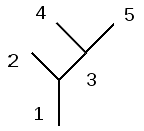
\includegraphics[scale=.6]{explicit_example.pdf}
\caption{The clusters for the example equations (\ref{eq: explicit example}) viewed graphically.}
\label{fig: ExplicitExample}
\end{figure}

 \item In the ASYNCH source code and in this document, the clusters of variables are referred to as \emph{links}. Every link has a positive integer attached to it that identifies the link uniquely. This number is referred to as the \emph{link ID}. The unknowns in the clusters are referred to as the \emph{states of the link}.
 
 \item The term \emph{peakflow} is used frequently with ASYNCH. This is a hydrological term, but it can take meaning in other applications. A peakflow of a state is the maximum value of that state over a period of time.

 \item The term \emph{model} is used frequently in technical disciplines to refer to a (usually mathematical) procedure or computer program for obtaining a description for how a natural process works. In this documentation, a model refers to the collection of equations, \emph{but not their solution}. The entire purpose of ASYNCH is to solve ODEs efficiently, thus producing their solution. No model created for ASYNCH should ever contain time steps. The equations (\ref{eq: explicit example}) are an example of a model.
 
 \item Each model has a number of states that are to be determined at each link. At a specific time, these states are stored in a vector, known as a \textit{state vector}. Similarly, the value of the differential and algebraic equations at a particular time and state are stored in an \textit{equation-value vector}. There is a correspondence between state and equation-value vectors at each link. For example, if the underlying model is a system of differential equations, then the derivative of the first state in a state vector is stored in the first entry of the equation-value vectors, the derivative of the second state in a state vector is stored in the second entry of the equation-value vectors, etc.
 
 As an example, a state vector for equations (\ref{eq: explicit example}) will look like
 \begin{align*}
  \left[ y_1,\ y_2,\ y_3,\ y_4,\ y_5,\ y_6,\ y_7,\ y_8,\ y_9,\ y_{10} \right]^T
 \end{align*}
 while an equation-value vector will look like
 \begin{align*}
  \left[ \frac{dy_1}{dt},\ \frac{dy_2}{dt},\ \frac{dy_3}{dt},\ \frac{dy_4}{dt},\ \frac{dy_5}{dt},\ \frac{dy_6}{dt},\ \frac{dy_7}{dt},\ \frac{dy_8}{dt},\ \frac{dy_9}{dt},\ \frac{dy_{10}}{dt} \right]^T
 \end{align*}

 
 \item Some models contain discontinuities in their equations. This can include not only the equation themselves, but also in their derivatives. ASYNCH supports intelligent handling of these abrupt changes when the equations can be described piecewise. For example, the differential equation
 \begin{align*}
  \frac{dy}{dt} &= \left\{ \begin{array}{c} -(y-5) + f(t), \mbox{for } y < 5 \\
                            -(y-5)^2 + f(t), \mbox{for } y \geq 5
                           \end{array} \right.
 \end{align*}
 with some forcing function $f$, has a discontinuity in the derivative of $y$. Each component of the piecewise function is referred to as a \emph{discontinuity state}.
 
 \item A few computer related terms are thrown around frequently in this document (and in parallel computing in general) that are worth describing.
 \begin{itemize}
  \item A \emph{node} is a physical computer. This includes any related hardware inside the computer (cores, memory, hard disks, etc). The term \emph{cluster} is used to refer to an interconnected group of nodes.
  \item A \emph{core}, \emph{processor}, or \emph{slot} (in the case of Iowa HPC resources) are the physical processing units in computers. These are the components that actually perform computations.
  \item A \emph{process} is an instance of a running program. ASYNCH uses MPI processes to achieve parallelism. This means several instances of ASYNCH are run simultaneously, each able to communicate with each other. Because this document refers to ASYNCH, the phrase \emph{MPI process} is interchangeable with process. It is simply used to emphasize that communication occurs with MPI.
  \item A \emph{thread} is a sequence of instructions (code) to a processor. \emph{Multithreading} is when many threads are created by a program and potentially executed simultaneously on a single node. ASYNCH does not currently support multithreading explicitly (it may occur ``behind the scenes'' in MPI, however).
 \end{itemize}
 Generally with ASYNCH, a one-to-one correspondence between the number of cores and processes is desired. More processes than cores means some cores must run more than one process, creating computational bottlenecks. More cores than processes means some cores will have no work to complete.
 
\end{itemize}


\section{Quickstart Guide and Example Simulations} \label{sec: quickstart}

In this section, we will give the steps and data needed for running basic simulations. This section is intended for getting a new user up and running quickly, and to provide links in this documentation for more information when needed.

First, be sure to follow the steps in Section \ref{sec: source code, compiling, and running asynch} for installing the ASYNCH solvers. For those using Iowa HPC resources, downloading and compiling the source code is not necessary.

The ASYNCH directory contains a folder called \emph{examples}, which contains several data files for starting sample simulations, as well as sample outputs for comparision. For Iowa HPC users, the ASYNCH directory is 
\begin{codeindent}
/Groups/IFC/Asynch/
\end{codeindent}
The \emph{examples} directory should be copied to a location where the user has write access (for example, the home directory). On Helium or Neon, this can be done with
\begin{codeindent}
 cp -r /Groups/IFC/Asynch/examples/ $\sim$/
\end{codeindent}


For the first example, we will produce output for a small basin with 11 links using a hydrological model with constant runoff. The global file to setup this simulation is \emph{Global190.gbl}. This uses the model given in Section \ref{sec: constant runoff model}. If using your own machine, the simulation can be run with the command
\begin{codeindent}
 mpirun -np 1 <bin path>/ASYNCH Global190.gbl
\end{codeindent}
If using Iowa HPC resources, use the appropriate binary path:
\begin{codeindent}
 /Groups/IFC/Asynch/bin\_helium/ \\
 /Groups/IFC/Asynch/bin\_neon/
\end{codeindent}
As calculations are performed, you will see output produced to the terminal window. If using Helium or Neon (or any system using the Sun Grid Engine), the submit script \emph{test.sh} can be used to run the simulation. Use the command
\begin{codeindent}
 qsub test.sh
\end{codeindent}
while in the \emph{examples} directory to launch the job. Output from the program will be produced in a log file with a name like \emph{test\_run.o\#\#\#\#\#\#}. Try using the command
\begin{codeindent}
 qstat -u <username>
\end{codeindent}
to monitor the progress of your job.

\textbf{Warning: A submit script is needed to run a job on multiple machines of Iowa HPC resources. If you attempt to run an ASYNCH simulation using just \emph{mpirun} at a terminal window, you are probably running ASYNCH on a login node. Doing this limits the number of cores available to 12, slows down all other users' connections, and is an easy way to be reported to the HPC admins for misuse of resources!}

When the program is complete, the output results are written to the folder \emph{examples}. The global file causes the production of three output files: \emph{test.dat}, \emph{test.pea}, and \emph{test.rec}. These files should be identical to those found in \emph{examples/results}. The .dat file contains the output hydrograph for links with link ids 3 and 80. The .pea file contains the peakflow information for every link. The .rec file contains the final value of every state of every link at the end of the simulation. For this simulation, all output files are small enough to view in a text editor.

The simulations performed will use only 1 MPI process. To increase this number, use, for example,
\begin{codeindent}
 mpirun -np 2 <ASYNCH directory>/ASYNCH Global190.gbl
\end{codeindent}
or modify \emph{test.sh} to use more processes. This can be done by modifying
\begin{codeindent}
 \#\$ -pe orte 1
\end{codeindent}
to use 2 processes instead of 1. Also be sure to modify the last line with \emph{mpirun} so MPI looks for 2 processes.

When using more than 1 process, your results may differ slightly from those in \emph{examples/results}. In fact, the results may vary slightly from simulation to simulation, even if nothing changed in the global file. This is a result from the asynchronous communication used by ASYNCH for MPI processes and is an expected behavior.

\begin{figure}[ht]
\centering
\includegraphics[scale=.5]{link80.pdf}
\includegraphics[scale=.5]{link3.pdf}
\caption{Output from the sample simulation.}
\label{fig: sample hydrographs}
\end{figure}

\begin{figure}[ht]
\centering
\includegraphics[scale=.5]{cclink2527_q.pdf}
\includegraphics[scale=.5]{cclink2527_base.pdf}
\caption{Output from the toplayer model sample simulation.}
\label{fig: sample hydrographs cc}
\end{figure}

As a second example, try the same procedure as before using the global file \emph{Global254.gbl}. If using an Iowa HPC resource, the submit script \emph{clearcreek.sh} can be used. The model for this simulation is the toplayer hydrological model using the Clear Creek river basin. See Section \ref{sec: top layer hydrological model}. Results for the output discharge and baseflow are given in Figure \ref{fig: sample hydrographs cc}. This basin is larger than in the previous simulation as it contains about 6,000 links. This is a good example to experiment with the number of processes used. A time series of the channel discharge and baseflow at the outlet are given in Figure \ref{fig: sample hydrographs cc}.


\section{Iowa HPC Resources} \label{sec: iowa hpc resources}

The University of Iowa offers access to two high performance computing resources: the Helium and Neon clusters. A user of these clusters will have access to different sets of machines (called \emph{queues}) depending upon their affiliation with the University. Each of these clusters uses the \emph{Sun Grid Engine} (or SGE) for scheduling program runs (called \emph{jobs}), so any simulations performed with ASYNCH on an Iowa HPC resource MUST be accompanied by an SGE submit script. This section gives a brief introduction to submitting jobs on Helium and Neon.

Information about the clusters can be found in the online documentation:
\begin{codeindent}
\raggedright
Helium:

\url{https://www.icts.uiowa.edu/confluence/display/ICTSit/Helium+Cluster+Overview+and+Quick+Start+Guide}

Neon:

\url{https://wiki.uiowa.edu/display/hpcdocs/Neon+Overview+and+Quick+Start+Guide}
\end{codeindent}


\subsection{Input and Output} \label{sec: input and output}

The Helium and Neon clusters provide a network file system for storing files. Regardless of which nodes are used, all data written to these file systems are accessible to all machines on the cluster. Any input or output data files can be moved to or from the clusters with tools such as ftp or scp.

While a job is running, any information written to \emph{stdout} is stored in an output log file. The filename of this log file is set in the submit script. See Section \ref{sec: submit scripts}. The extension of the log files is of the format \emph{.o\#\#\#\#\#\#}, where the numbers after the \emph{.o} are given by the job id of the job. See Section \ref{sec: sge commands} for commands to find the job id. Typically, there is a delay in when data is written to \emph{stdout} and when it appears in the log file. When a job terminates successfully, all data written to \emph{stdout} is flushed to the log file.


\subsection{Queues} \label{sec: queues}

A complete list of available queues is given at \url{https://wiki.uiowa.edu/display/hpcdocs/Queue+Usage+and+Policies}. We present in this section a description of queues that a user of ASYNCH is likely able to access. See Figure \ref{fig: helium queues} for sample queues on Helium.

\begin{figure}
\centering
\begin{tabular}{|c|c|c|}
 \hline
 Queue Name & Cores & Investor \\
 \hline
 IFC & 10 Nodes, 8 cores each & Iowa Flood Center \\
 COE & 6 Nodes, 8 cores each & College of Engineering \\
 UI & 153 Nodes, 12 cores each & University of Iowa \\
 all.q & All of Helium & - \\
 \hline
 \end{tabular}
\caption{Sample queues on Helium.}
\label{fig: helium queues}
\end{figure}

If a user has access to an investor queue (for example, IFC or COE), then that user's jobs have priority on the nodes of that queue above any other users' jobs who do not have priority. This means Helium or Neon will terminate their jobs to allow yours to run. If multiple users have priority, then the order in which their jobs run is dependent upon resources available, how long a job has been waiting to run, etc. Investor queues are generally the nicest to use, provided other users with access are not running many jobs.

The University of Iowa has purchased nodes on both Helium and Neon, and made their use available to the entire university. These nodes can be accessed by anyone through the UI queue. Running jobs on this queue is the same as running jobs in an investor queue, except everyone with a Helium or Neon account has priority. This queue has many resources available, but tends to be in high demand. Using this queue typically requires a significant delay in when the job runs.

A special queue called \emph{all.q} is available to all users of Helium and Neon. When a job is submitted to this queue, it may be run on any available nodes, regardless of a user's priority level. This queue has the most resources available. However, if your job runs on nodes where you do not have priority, the job may be terminated when another user wishes to access the nodes. Running in the \emph{all.q} queue is always risky.

\subsection{SGE Commands} \label{sec: sge commands}

Several commands for SGE may be used at the Linux command line to help monitor jobs. A few of them are described here.

\begin{codeindent}
 qstat -u <username>
\end{codeindent}
This displays the current status of all jobs submitted by someone with the given username. This includes all running jobs as well as all jobs waiting to run.

\begin{codeindent}
 qstat -q <queue>
\end{codeindent}
This displays all jobs running or waiting to run in the given queue.

\begin{codeindent}
 qsub <submit script name>
\end{codeindent}
This submits to SGE a submit script to run, producing a job. A job submitted with qsub will typically wait some amount of time before running, even if resources are available.

\begin{codeindent}
 qdel <job id>
\end{codeindent}
This aborts a job. If the job is waiting to run, it will be removed immediately. If the job is running, aborting the job and freeing the compute resources may take a few minutes. The job id can be obtained with a call to one of the qstat commands above. For obvious reasons, a user can only abort their own jobs.

\subsection{Submit Scripts} \label{sec: submit scripts}

All jobs run on Helium and Neon must be started with the use of the \emph{qsub} command, which requires a \emph{submit script}. This script tells Sun Grid Engine (SGE) what resources are needed for the job, as well as what program is to be run. The following is an example of a typical submit script for running ASYNCH simulations, with a few extra commands commented out:
\begin{codeindent}
\#!/bin/sh

\#\$ -N test\_run

\#\$ -j y

\#\$ -cwd

\#\$ -m e

\#\$ -M user@uiowa.edu

\#\$ -pe orte 8

\#\#\#\#\$ -pe 8cpn 8

\#\#\#\#\$ -l mf=16G

\#\$ -l ib=1

\#\#\#\#\$ -q UI

\#\$ -q IFC

\#\#\#\#\$ -q all.q

\#\#\#\#\$ -q COE

mpirun -np 8 ./ASYNCH examples/Global254.gbl
\end{codeindent}

Lines starting with a \# indicate a resource related request to SGE. Four \# symbols indicates a comment. After the SGE requests, commands from a typical bash script are given, which indicate what the job will do.

Here is a quick description of the lines above that a typical user will need to change:

\begin{codeindent}
 \#\$ -N <job name>
\end{codeindent}
This specifies the name of the job. This name will appear in log files and in calls to qstat.

\begin{codeindent}
 \#\$ -m e

 \#\$ -M <email address>
\end{codeindent}
These lines are optional. When present, an email is sent to the given address when the job terminates (either successfully or unsuccessfully). This is useful for long running jobs.

\begin{codeindent}
 \#\$ -pe orte <number of cores>

 \#\$ -pe 8cpn <number of cores>
 
 \#\$ -pe 12cpn <number of cores>
\end{codeindent}
These commands indicate how many cores SGE should reserve. If using the parallel environment \emph{orte}, the cores will be selected from all available in the queue. The other two parallel environments \emph{8cpn} and \emph{12cpn} will use the cores from entire nodes. If some cores of a node are already in use, these environments will not reserve any cores from the nodes. The number of cores selected must be a multiple of 8 or 12, respectively. Only queues with 8 cores per node support \emph{8cpn}, and only queues with 12 cores per node support \emph{12cpn}.

\begin{codeindent}
 \#\$ -l mf=<memory amount>
\end{codeindent}
This command tells SGE to only run jobs on nodes with the specified amount of memory available. This command is only needed when running jobs in the \emph{UI} or \emph{all.q} queues with the \emph{orte} parallel environment. The memory amount should specify both the amount and units. So for example, 16G means 16 gigabytes and 8M means 8 megabytes. It's worth nothing that this command does not actually reserve the memory for your job. If this command is specified with 16G, and such a node is found, another job may be run at a later time which takes this memory from your job. Since most memory allocation in ASYNCH occurs in the init routines, this is seldom an issue.

\begin{codeindent}
 \#\$ -q <queue>
\end{codeindent}
This command tells SGE to run the job in the specified queue. If this command is not present, then \emph{all.q} is used (on Iowa HPC clusters).

Although these commands are typically specified in the submit script, they can be passed through command line arguments to \emph{qsub}. For example,
\begin{codeindent}
 qsub test.sh -q COE
\end{codeindent}
will submit the job defined through the submit script \emph{test.sh} to the queue \emph{COE}, \textbf{regardless of the queue specified in the submit script}. This can be useful for creating bash scripts to submit a large number of jobs to SGE.

Further, multiple commands to run programs may be given in the submit scripts. They are executed serially (i.e. one at a time). So if the submit script above instead ended with the commands
\begin{codeindent}
 mpirun -np 8 ./ASYNCH examples/Global254.gbl
 
 mpirun -np 8 ./ASYNCH examples/Global190.gbl
\end{codeindent}
then the cluster will run an ASYNCH simulation using \emph{Global254.gbl}. Once this simulation is complete, the cluster will run an ASYNCH simulation using \emph{Global190.gbl}. Both of these simulations will have output directed to the same log file, and will use the same cores and nodes requested earlier in the submit script.

Lastly, we point out that the number of cores requested through SGE can differ from the number of MPI processes ASYNCH uses. For example, a submit script could contain the lines
\begin{codeindent}
 \#\$ -pe 12cpn 12

 mpirun -np 5 ./ASYNCH examples/Global254.gbl
\end{codeindent}
SGE will reserve 12 cores, but only 5 are actually used. Similarly, the number of MPI processes could be larger than the requested number of cores. When this happens, some cores will execute multiple processes (not at the same time, of course). For most runs with ASYNCH, the cores reserved should equal the number of MPI processes.



\section{Input/Output Formats} \label{sec: input/output formats}

Numerous inputs are required to construct and solve the model equations. This includes link connectivity, link parameters, numerical error tolerances, precipitation forcings, a mathematical model, etc. Most inputs are specified on a link-by-link basis, and can be given as either a file or a database table.

In addition, ASYNCH must know information about data outputs. This includes where to store the outputs, what the outputs are, at which links outputs will be given, etc.

The format for each input and output is described below. For database inputs/outputs, ASYNCH can access PostgreSQL through the libpq libraries. Obviously, the user must have read or write permissions to a PostgreSQL database to utilize database features.

\subsection{Global File Structure} \label{sec: global file structure}

Global files (.gbl) are used to specify ALL inputs for the solvers. This includes river network topology files, database connections, initial model states, what information is printed to output files, model forcings, etc. Global files have a very rigid structure, unlike XML files, and information must be specified in a particular order. \textbf{The description of each input of the global files below are given in the order in which they are to be specified in the actual file}.

Global files are always ASCII files, assumed to be in UNIX format. The percent sign (\%) is used for single line comments. As described below, certain inputs are expected to be given within a single line. Other than this restriction, white space is ignored. Arguments surrounded by \{ \} below are mandatory, while those surrounded by the square brackets [ ] are dependent upon values specified by other parameters.

Although each setting in a global file modifies values for the ASYNCH solvers, their exact use can be modified by the user altering the underlying source code. This can be done with calls to routines described in Section \ref{sec: user interface routines}.

\subsubsection{Model Type and Maxtime} \label{sec: model type and maxtime}

\begin{codeindent}
Format: \\
\{model id\} \{total simulation time\}
\end{codeindent}

The first value specifies the id for the model to be used. This is a nonnegative integer value which corresponds to a particular system of ordinary-differential equations (or possibly DAEs). Examples of built-in models is given in Section \ref{sec: example models}. For custom models, this model id is ignored. See Section \ref{sec: custom models}.

The second is the total simulated time used by the solvers. This is a floating point number. The units are generally in minutes, however, some models can get away with using other units (seconds, hours, etc) if carefully crafted. All built in models use minutes for the time.

\subsubsection{Parameters on Filenames} \label{sec: parameters on filenames}

\begin{codeindent}
 Format: \\
 \{parameter on output filename flag\}
\end{codeindent}

This is a boolean value (0 or 1) that indicates whether all output filenames should include the uniform in space and time parameters. 0 indicates no, 1 indicates yes. This feature can be useful for keeping track of output files from multiple simulations.

\subsubsection{Solver Outputs} \label{sec: solver outputs}

\begin{codeindent}
 Format: \\
 \{number of outputs\} \\
 {[}output1{]} \\
 {[}output2{]} \\
 {[}...{]}
\end{codeindent}

This set of input parameters specifies the names of all outputs from the solvers. Several built in outputs exist, and the user is able to construct his own outputs. Built in outputs are given in Section \ref{sec: built-in output time series}. Output names are case sensitive. The first required value is the number of outputs ($>=$ 0), followed by the names of each output, on separate lines.


\subsubsection{Peakflow Statistics Function Name} \label{sec: peakflow statistics function name}

\begin{codeindent}
 Format: \\
 \{function name\}
\end{codeindent}

This sets the function for outputting peakflow information. The built in peakflow function ``Classic'' is one option, and the user is free to construct his own. A function name must be specified here, even if peakflow information is not requested for any links.


\subsubsection{Global Parameters} \label{sec: global parameters}

\begin{codeindent}
 Format: \\
 \{number of parameters\} [parameter1] [parameter2] ...
\end{codeindent}

This is where model parameters which are constant in space and time are specified. The first value is a nonnegative integer specifying the number of global parameters to follow. Every model requires a certain number of global parameters. If the number given in the global file is less than expected for a particular model, an error occurs. If the number is greater than expected, a warning is given. These ``extra'' parameters are available to the model for use. This can sometimes be useful for quick tests, but should be avoided normally.

The parameter meanings depend upon the model used. The units of these parameters is also model dependent.

\subsubsection{Buffer Sizes} \label{sec: buffer sizes}

\begin{codeindent}
 Format: \\
 \{steps stored at each link\} \{max number of steps transferred\} \{discontinuity buffer size\}
\end{codeindent}

These nonnegative integer values allow the user to specify sizes of internal buffers. In general, as these numbers are increased, the solvers run faster, but more memory is required. A good starting point that works in most cases is the set 30 10 30. Typically, if these values need to be less than 10 to run the solvers, a deeper issue with memory constraints should be addressed.

\subsubsection{Topology} \label{sec: topology}

\begin{codeindent}
 Format: \\
 \{topology flag\} [output link id] \{.rvr filename or .dbc filename\}
\end{codeindent}

This is where connectivity of the river network is specified. This can be done in one of two ways. If the topology flag is 0, a river topology file (.rvr) is used. If the topology flag is 1, then topology is downloaded from the database specified with the .dbc filename. The database connection allows for one additional feature: a subbasin can be specified. If the output link id is taken to be 0, all link ids found in the database are used. Otherwise, the link with link id specified and all upstream links are used. Pulling subbasins from a topology file is not currently supported.

\subsubsection{Link Parameters} \label{sec: link parameters}

\begin{codeindent}
 Format: \\
 \{parameter flag\} \{.prm filename or .dbc filename\}
\end{codeindent}

This specifies where parameters which vary by link and not time, are specified. If the parameter flag is 0, the parameters are given in a parameter (.prm) file. If the flag is 1, then the parameters are downloaded from the database specified by the database connection file (.dbc). The number, order, meaning, and units of these parameters varies from model to model.


\subsubsection{Initial States} \label{sec: initial states}

\begin{codeindent}
 Format: \\
 \{initial state flag\} \{.ini, .uini, .rec, or .dbc filename\} [unix time]
\end{codeindent}

This section specifies the initial state of the model. The values for the initial state flag can be 0, 1, 2, or 3, corresponding, respectively, to a .ini, .uini, .rec, or .dbc file. The unix time argument is used for database connections only. This value is available in the query of the database connection file and can be used for selecting values from tables.


\subsubsection{Forcings} \label{sec: forcings}

\begin{codeindent}
 Format: \\
 \{number of forcings\} \\
 {[}forcing1 flag{]} {[}forcing1 information{]} \\
 {[}forcing2 flag{]} {[}forcing2 information{]} \\
 {[}...{]}
\end{codeindent}

Information about time dependent forcings is specified here. Each model has an expected number of forcings. If the number of forcings specified here is less than expected, an error is thrown. If the number of forcings is greater than expected, a warning is given. This warning allows for tests to be performed and implemented quickly. In general, this feature should be avoided.

Forcing information varies considerably based upon the corresponding forcing flag. Several forcing types require unix times to determine what forcing data to use. If a model requires multiple forcings with unix times, the times \emph{do not} need to be consistent, i.e., one forcing could start on July 1st 2014 at midnight, while another forcing starts at April 5th 2008.

%\subsubsection{No Forcing} \label{sec: no forcing}
\paragraph{No Forcing} \label{sec: no forcing}

\begin{codeindent}
Format: \\
 0
\end{codeindent}

A forcing flag of 0 specifies no forcing input. This is the same as a forcing value of 0.0 for all links and all time.

\paragraph{Storm File} \label{sec: storm file}

\begin{codeindent}
 Format: \\
 1 \{.str filename\}
\end{codeindent}

A forcing flag of 1 indicates the forcing is specified by a .str file. The filename and path of a valid storm (.str) file required.

\paragraph{Binary Files} \label{sec: binary files}

\begin{codeindent}
 Format: \\
 2 \{binary file identifier\} \\
 \{chunk size\} \{time resolution\} \{beginning file index\} \{ending file index\}
\end{codeindent}
 
 A forcing flag of 2 indicates the forcing is specified by a collection of binary forcing files. The identifier can be adorned with a path to the binary files. The chunk size is a positive integer that indicates the number of binary files kept in memory at once. The time resolution indicates the amount of time between successively indexed binary files. This value is a floating point number with units equal to those of the time variable of the model used. The beginning and ending file indices indicate the range of the binary files to be used. The indices are integer valued.
 
 The simulation will begin using the binary file with index given by the beginning file index. If the total simulation time would require binary files with index greater than the ending file index, the forcing values are taken to be 0.0 for all such binary files.
 
\paragraph{Forcings from Databases} \label{sec: forcings from db}
 
\begin{codeindent}
 Format: \\
 3 \{.dbc filename\} \\
 \{chunk size\} \{time resolution\} \{beginning unix time\} \{ending unix time\}
\end{codeindent}

A forcing flag of 3 indicates the forcing data will be pulled from a PostgreSQL database. The database connection filename can include a path. The chunk size is a positive integer representing the number of forcing values pulled from the database at once from each link. A chunk size of 10 tends to work well. A larger chunk size requires more memory and larger datasets returned from the database, but a small number of queries. The time resolution is a floating point number with units in minutes. This represents the time resolution of the data in the accessed table. The integrity of the database table is not thoroughly checked by the solvers.

The simulation will begin using the data from the database with unix time given by the beginning unix time. If the total simulation time would require data from the database with unix time greater than the ending unix time, the forcing values are taken to be 0.0 for times greater than the ending unix time.


\paragraph{Uniform Forcings} \label{sec: uniform forcings}
 
\begin{codeindent}
 Format: \\
 4 \{.ustr filename\} 
\end{codeindent}

A forcing flag of 4 indicates a forcing that is uniform in space. The forcings are given by a uniform storm file (.ustr).


\paragraph{GZipped Binary Files} \label{sec: gzipped binary files}

\begin{codeindent}
 Format: \\
 6 \{gzipped binary file identifier\} \\
 \{chunk size\} \{time resolution\} \{beginning file index\} \{ending file index\}
\end{codeindent}
 
 A forcing flag of 6 indicates the forcing is specified by a collection of binary forcing files that have been gzipped (compressed as .gz files). All parameters for this flag are identical to that of using binary files with forcing flag 3.

 
\paragraph{Monthly Forcings} \label{sec: monthly forcings}

\begin{codeindent}
 Format: \\
 7 \{.mon filename\} \\
 \{beginning unix time\} \{ending unix time\}
\end{codeindent}

A forcing flag of 7 indicates a uniform in space forcing that recurs monthly. When the end of the calendar year is reached, the monthly forcing file (.mon) is read again from the beginning. The beginning unix time is used to determine the month the simulation begins (for this forcing). If the total simulation time takes the simulation past the ending unix time, the forcing is assumed to be 0.0 for all locations and times beyond the ending unix time.

\paragraph{Grid Cell Files} \label{sec: grid cell files}

\begin{codeindent}
 Format: \\
 8 \{index filename\} \\
 \{chunk size\} \{beginning file index\} \{ending file index\}
\end{codeindent}
 
A forcing flag of 8 indicates the forcing is specified by a collection of grid cell forcing files. The index filename can be adorned with a path to the index file. The chunk size is a positive integer that indicates the number of grid cell files kept in memory at once. The beginning and ending file indices indicate the range of the grid cell files to be used. The indices are integer valued.
 
The simulation will begin using the grid cell file with index given by the beginning file index. If the total simulation time would require grid cell files with index greater than the ending file index, the forcing values are taken to be 0.0 for all such grid cell files. In addition, if a grid cell file is missing, all values at each cell are assumed to be 0.0.

\subsubsection{Dams} \label{sec: dams}

\begin{codeindent}
 Format: \\
 \{dam flag\} [.dam or .qvs filename]
\end{codeindent}

This section specifies whether dams will be used. A dam flag of 0 means no dams are used. A flag of 1 indicates a dam file (.dam) will be used, and a flag value of 2 indicates a discharge vs storage file (.qvs) will be used. Some models do not support dams. For these models, the dam flag must be set to 0 or an error occurs.

\subsubsection{State Forcing Feeds} \label{sec: state forcing feeds}

\begin{codeindent}
 Format: \\
 \{reservoir flag\} [.rsv or .dbc filename] [forcing index]
\end{codeindent}

This section specifies whether a provided forcing (Section \ref{sec: forcings}) is to be used as a forcing of the states of differential or algebraic equations at some links. A reservoir flag of 0 indicates no forcing will by applied to system states. A flag of 1 indicates state forcings will be applied to all link ids in the specified .rsv file. A reservoir flag of 2 indicates state forcing will be applied to all link ids pulled from the database the given .dbc file. If the reservoir flag is not 0, then the index of the forcing must be specified.


\subsubsection{Time Series Location} \label{sec: time series location}

\begin{codeindent}
 Format: \\
 \{time series flag\} [time resolution] [.dat / .csv / .dbc filename] [table name]
\end{codeindent}

This section specifies where the final output time series will be saved. A time series flag value of 0 indicates no time series data will be produced. Any flag with value greater than 0 requires a time resolution for the data. This value has units equal to the units of \textit{total simulation time} (typically minutes). A value of -1 uses a resolution which varies from link to link based upon the expression
\begin{align}
 \left(0.1 \cdot \frac{A}{1 \ km^2} \right)^{\frac{1}{2}} \ min
\end{align}
where $A$ is the upstream of the link, measured in $km^2$.

A time series flag of 1 indicates the results of the simulation will be saved as a .dat file. The filename complete with a path must be specified. If a file with the name and path given already exists, it is overwritten. A time series flag of 2 indicates the results will be stored as a .csv file. A time series flag of 3 indicates the results will be uploaded into the database described by the given .dbc. In this case, a table name accessible by the queries in the .dbc file must be specified.

This section is independent of the section for \textit{Link IDs to Save} described below (Section \ref{sec: link ids to save}). For example, if link ids are specified in the \textit{Link IDs to Save} section and the \textit{time series flag} in the \textit{Time Series Locations} set to 0, no output is generated. Similarly, if the \textit{time series id flag} is set to 0 in the \textit{Link IDs to Save} section and the \textit{time series flag} is set to 1, a .dat file with 0 time series is produced.

\textbf{Notice: the \emph{time resolution} is entirely independent of the time step used by the numerical integrators. Reducing this value does NOT produce more accurate results. To improve accuracy, reduce the error tolerances described in Section \ref{sec: numerical error tolerances}. There is no built-in way to produce results at every time step, as this is a very easy way to crash a compute node or file system.}

\subsubsection{Peakflow Data Location} \label{sec: peakflow data location}

\begin{codeindent}
 Format: \\
 \{peakflow flag\} [.pea / .dbc filename] [table name]
\end{codeindent}

This section specifies where the final peakflow output will be saved. A peakflow flag of 0 indicates no peakflow data is produced. A peakflow flag of 1 indicates the peakflow results of the simulation will be saved as a .pea file. The filename complete with a path from the binary file must be specified. A peakflow flag of 2 indicates the results will be uploaded into the database described by the given .dbc. In this case, a table name accessible by the queries in the .dbc file must be specified.

This section is independent of the section for \textit{Link IDs to Save} described below (Section \ref{sec: link ids to save}). For example, if link ids are specified in the \textit{Link IDs to Save} section and the \textit{peakflow flag} in the \textit{Peakflow Data Location} is set to 0, no output is generated. Similarly, if the \textit{peakflow id flag} is set to 0 in the \textit{Link IDs to Save} section and the \textit{peakflow flag} is set to 1, a .pea file with 0 peakflows is produced.


\subsubsection{Link IDs to Save} \label{sec: link ids to save}

\begin{codeindent}
 Format: \\
 \{time series id flag\} [.sav / .dbc filename] \\
 \{peakflow id flag\} [.sav / .dbc filename]
\end{codeindent}

This section provides the list of link ids in which data is produced. The first line is for the time series outputs, while the second is for the peakflow outputs. The \textit{time series ID flag} and the \textit{peakflow ID flag} take the same list of possible values. A flag of 0 indicates no link IDs for which to produce data. A flag of 1 indicates the list of link IDs is provided by the corresponding save file (.sav). A flag of 2 indicates the list of link IDs is provided by the database specified in the given database connection file (.dbc). A flag of 3 indicates that all links will have data outputted.

\textbf{Warning: a \emph{time series ID flag} of 3 can easily wreak havoc on a file system for simulations with a large number of links. At the very least, extremely large output files and database tables will occur. Be very careful with this!}

Typically, using a flag value of 3 for peakflow link ids, or for the time series ID flag for a very small basin (< 500 links) will not create any problems.

This section is independent of the sections for \textit{Time Series Location} and \textit{Peakflow Data Location} above (Sections \ref{sec: time series location} and \ref{sec: peakflow data location}). For example, if link ids are specified in the \textit{Link IDs to Save} section and the \textit{time series flag} in the \textit{Time Series Location} set to 0, no output is generated. Similarly, if the \textit{time series id flag} is set to 0 in the \textit{Link IDs to Save} section and the \textit{time series flag} is set to 1, a .dat file with zero time series is produced.
 
 
\subsubsection{Snapshot Information} \label{sec: snapshot info}

\begin{codeindent}
Format: \\
\{snapshot flag\} [.rec / .dbc filename]
\end{codeindent}
 
This section specifies where snapshot information is produced. A snapshot is a record of every state at every link in the network. Snapshots are produced at the end of simulations. This is useful for beginning a new simulation where an old one ended. A snapshot flag of 0 indicates no snapshot is produced. A snapshot flag of 1 indicates the snapshot will be produced as a recovery (.rec) file with path and filename specified. A snapshot flag of 2 indicates the snapshot will be uploaded to the database specified by the database connectivity (.dbc) file.

\subsubsection{Scratch Work Location} \label{sec: scratch work location}

\begin{codeindent}
Format: \\
\{filename\}
\end{codeindent}

This section specifies the location of temporary files. These files are used to store intermediate calculations. The filename can include a path name. If the file already exists, the contents are overwritten.

If a simulation is aborted, these files may not be removed. Otherwise, they are deleted at the end of the simulation.
 
\subsubsection{Error Control Parameters} \label{sec: error control parameters}

\begin{codeindent}
Format: \\
\{facmin\} \{facmax\} \{fac\}
\end{codeindent}

This section specifies parameters related to the error control strategy of the numerical integrators. The value \textit{facmin} represents the largest allowed decrease in the stepsize of the integrators as a percent of the current step. Similarly, \textit{facmax} represents the largest allowed increase. The value \textit{fac} represents the safety factor of the integrators. Any accepted stepsize is multiplied by this value. Good values of \textit{facmin}, \textit{facmax}, and \textit{fac} to use are 0.1, 10.0, and 0.9, respectively.

\subsubsection{Numerical Error Tolerances} \label{sec: numerical error tolerances}

\begin{codeindent}
Format: \\
\{solver flag\} [.rkd filename] \\
{[}rk solver index{]} \\
{[}absolute error tolerance 1{]} {[}absolute error tolerance 2{]} ... \\
{[}relative error tolerance 1{]} {[}relative error tolerance 2{]} ... \\
{[}dense absolute error tolerance 1{]} {[}dense absolute error tolerance 2{]} ... \\
{[}dense relative error tolerance 1{]} {[}dense relative error tolerance 2{]} ...
\end{codeindent}

This section specifies error tolerances for the numerical integrators. A \textit{solver flag} of 0 indicates the same tolerances will be used for all links. A \textit{solver flag} of 1 indicates the tolerance info will be specified in the given RK data (.rkd) file.

If \textit{solver flag} is 0, than an \textit{rk solver index} must be specified. A list of Runge-Kutta methods is given in Section \ref{sec: built-in runge-kutta methods}. Each error tolerance must have a value for each state of the system. The order of the tolerances must match the order of the states in the state vectors. The absolute and relative error tolerances are those typically used for RK methods. The dense tolerances are for the numerical solution produced between time steps. A numerical solution is rejected if either the error tolerances or dense error tolerances for any state is believed to be violated.


\subsection{Database Connection Files} \label{sec: database connection files}

Database connection files are ASCII text files with a .dbc extension which specify how to connect to a database, and the queries to pull/push data from/to the database. Although the format of database connection files is the same, the specific requirements of the queries varies with how the file is used. For instance, queries for pulling link connectivity information is very different from queries for uploading peakflows to a database table.
\begin{codeindent}
 Format:
 
 dbname=\{db\} host=\{host\} user=\{user\} password=\{pass\}
 
 \{number of queries\}
 
 [query 1]
 
 [query 2]
 
 ...
\end{codeindent}
The first line of every database connection file specifies the information needed to make a connection. A user must have permission to read or write from the database at the given host; otherwise, queries sent to the database will fail. The number of queries will vary depending upon how the database connection file is used. The appropriate number of queries and what they should return is documented in the remainder of Section \ref{sec: input/output formats}. The number of queries may be zero.

Any queries listed \emph{MUST} be ended with a semicolon (;). For some queries, further information outside the database connection file may be available, depending upon how the query is to be used. This additional information is explained in the appropriate section below for input formats. Such information includes link ids and unix times. To denote in a query where this information should be placed, use the symbol ``\%u'' for integers and ``\%s'' for names.


\subsection{Link Connectivity Input} \label{sec: link connectivity input}

Link connectivity information is used to specify how links in a network are connected. Connectivity can be provided through either a river network file (.rvr) file or through a database table. When a river network file is used, every link in the file is used (i.e. no subnetworks). When pulling connectivity data from a database, a subset of the network can be used.

Regardless of the format, all link ids must be given in the same order in the link connectivity, link parameter, and initial state inputs.

River network files are ASCII text files with the following format:
\begin{codeindent}
 \{number of links\}
 
 \{link id 1\}
 
 \{number of parents\} [parent id 1] [parent id 2] ...
 
 \{link id 2\}
 
 \{number of parents\} [parent id 1] [parent id 2] ...
 
 ...
\end{codeindent}
White space can be used freely throughout the file. The layout in the above specification is purely optional; the order of the information is what is important. The file begins with the total number of links in the file. Then each link id is specified, followed by the number of parents for the link and each of their ids. A link id can appear in a list of parent link ids at most once. If a link does not have parents, it must still appear in this file with a 0 for the number of parents.

If the connectivity is pulled from a database, a corresponding database connection file is used. This file requires three queries:
\begin{itemize}
 \item Query to pull all link ids from a table. 
  \begin{itemize}
   \item Inputs: none
   \item Returned tuples: (link id)
  \end{itemize}
 \item Query to pull all link id, parent link id pairs
  \begin{itemize}
   \item Inputs: none
   \item Returned tuples: (link id, parent link id)
  \end{itemize}
 \item Query to pull all link id, parent link id pairs upstream from a given outlet link id
  \begin{itemize}
   \item Inputs: outlet link id
   \item Returned tuples: (link id, parent link id)
  \end{itemize}
\end{itemize}
The last two queries must return a tuple for each link id for each parent link. So a link with two parents should appear twice in the returned tuples, once for each parent link. The returned tuples must be grouped by the link id so all parent information appears consecutively.


\subsection{Link Parameter Input} \label{sec: link parameter input}

Link parameter input specifies the parameters for the model that vary link to link. This information can be provided in a parameter file (.prm) or through a database table. The number of parameters for each link, their meaning, and their order depends upon the model used. In particular, the value of \emph{disk\_params} determines the number of parameters expected at each link. See Section \ref{sec: setparamsizes}.

Regardless of the format, all link ids must be given in the same order in the link connectivity, link parameter, and initial state inputs.

A parameter file is an ASCII text file with the following format:
\begin{codeindent}
 \{number of links\}
 
 \{link id 1\}
 
 \{parameter 1\} \{parameter 2\} \{parameter 3\} ...
 
 \{link id 2\}
 
 \{parameter 1\} \{parameter 2\} \{parameter 3\} ...
 
 ...
\end{codeindent}
White space can be used freely throughout the file. The layout in the above specification is purely optional; the order of the information is what is important. The file begins with the total number of links. Then each link id is specified, followed by the parameters for that link.

If the parameters are pulled from a database, a corresponding database connection file is used. This file requires two queries:
\begin{itemize}
 \item Query to pull all parameters. 
  \begin{itemize}
   \item Inputs: none
   \item Returned tuples: (link id, parameter 1, parameter 2, ...)
  \end{itemize}
 \item Query to pull all parameters above an outlet.
  \begin{itemize}
   \item Inputs: outlet link id
   \item Returned tuples: (link id, parameter 1, parameter 2, ...)
  \end{itemize}
\end{itemize}


\subsection{Initial Values Input} \label{sec: initial values input}

The link initial values input specifies the initial values for the states of the differential and algebraic model equations. This information can be provided in several different formats: an initial value file (.ini), a uniform initial value file (.uini), a recovery file (.rec), and through a database table.

An initial value file is an ASCII text file that lists the initial values for each link. The format is:
\begin{codeindent}
 \{model type\}
 
 \{number of links\}
 
 \{initial time\}
 
 \{link id 1\}
 
 \{initial value 1\} \{initial value 2\} ...
 
 \{link id 2\}
 
 \{initial value 1\} \{initial value 2\} ...
 
 ...
\end{codeindent}
The model type is the number of the model to be used. This determines how many initial values are expected for the model. Initial states must be provided only for those states determined by differential equations, and only for those which require an initial condition. These are the states with index between \emph{diff\_start} and \emph{no\_ini\_start} in the state vectors. See Section \ref{sec: setparamsizes}.

A uniform initial value file is similar to an initial value file, but the initial values, when required, are the same at every link. The format is given by:
\begin{codeindent}
 \{model type\}
 
 \{initial time\}
 
 \{initial value 1\} \{initial value 2\} ...
\end{codeindent}
The model type is the number of the model to be used. This determines how many initial values are expected for the model. Initial values must be provided only for those states determined by differential equations, and only for those which require an initial condition. These are the states with index between \emph{diff\_start} and \emph{no\_ini\_start} in the state vectors. See Section \ref{sec: setparamsizes}. Notice that unlike an initial value file, no link ids are given, and only one set of initial values are given.

A recovery file is an ASCII text file that lists the initial values for each link. The format is:
\begin{codeindent}
 \{model type\}
 
 \{number of links\}
 
 \{initial time\}
 
 \{link id 1\}
 
 \{initial value 1\} \{initial value 2\} ...
 
 \{link id 2\}
 
 \{initial value 1\} \{initial value 2\} ...
 
 ...
\end{codeindent}
The format is identical to that of an initial value file, with one important exception. The initial value of \emph{EVERY} state must be provided at each link. For models with \emph{diff\_start} set to 0 and \emph{no\_ini\_start} set to \emph{dim}, a recovery file is identical to an initial value file. See Section \ref{sec: setparamsizes}. \textbf{Warning: For the initial values of algebraic equations, no checks on the input data are performed to ensure the solution is consistent}.

If the initial values are pulled from a database, a corresponding database connection file is used. This file requires one query:
\begin{itemize}
 \item Query to pull all initial states for every link. 
  \begin{itemize}
   \item Inputs: integer value
   \item Returned tuples: (link id, initial value 1, initial value 2, ...)
  \end{itemize}
\end{itemize}
The query allows for one input to be used to obtain the needed information. This value could be, for example, an outlet link id or a unix time. Similar to recovery files, initial values must be provided for every link.


\subsection{Forcing Inputs} \label{sec: forcing inputs}

Numerous and diverse formats are implemented for feeding forcing inputs into a model. These formats vary considerably, and can have different impacts on performance.

Storm files (.str) provide an ASCII text format for setting a forcing at each link. The format of these files is:
\begin{codeindent}
 \{number of links\}
 
 \{link id 1\} \{number of changes\}

 \{time 1\} \{value 1\}
 
 \{time 2\} \{value 2\}
 
 \{time 3\} \{value 3\}
 
 ...
 
 \{link id 2\} \{number of changes\}

 \{time 1\} \{value 1\}
 
 \{time 2\} \{value 2\}
 
 \{time 3\} \{value 3\}
 
 ...
\end{codeindent}
The format requires a time series to be provided for every link. The number of values can vary from link to link, and the time steps do not need to be uniformly spaced or even the same for each link. The first time at each link must be the same however, and correspond to the beginning of the simulation (typically 0). The forcings are assumed to be constant between time steps. After the final time step, the forcing value is held at the last value for the remainder of the simulation. The data provided by a storm file is entirely read into memory at the beginning of a run. As such, this format may not be suitable for large or long simulations.

Uniform storm files (.ustr) provide an ASCII text format for setting a forcing uniformly at each link. The format of these files is:
\begin{codeindent}
 \{number of changes\}

 \{time 1\} \{value 1\}
 
 \{time 2\} \{value 2\}
 
 \{time 3\} \{value 3\}
 
 ...
\end{codeindent}
The format is similar to that of a storm file, but only one time series is specified, and is applied at every link. The time steps do not need to be uniformly spaced. The first time must correspond to the beginning of the simulation (typically 0). The forcing is assumed to be constant between time steps. After the final time step, the forcing value is held at the last value for the remainder of the simulation. The data provided by a uniform storm file is entirely read into memory at the beginning of a run. As such, this format may not be suitable for extremely long simulations.


Binary storm files (no extension) may also be used. Instead of a single file, these are a collection of files providing forcing values at different times. The format of these is:
\begin{codeindent}
 \{link id 1 value\}
 
 \{link id 2 value\}
 
 \{link id 3 value\}
 
 ...
\end{codeindent}
Each file is simply a list of forcing values for each link. Because link ids are not present, the values are assumed to be in the same order as the link ids from the link connectivity input. Further, a value must be specified for every link.

The filename of each binary file should end with an integer value. The index of each file should be numbered consecutively. The time step size between files, as well as the range of files to use, are specified in the global file (see \ref{sec: binary files}). If the simulation goes beyond the last file, all further forcing values are assumed to be 0 for all links.

The values in binary storm files are stored as single precision floating point numbers, with endianness different from the native machine. These files are read into memory in blocks. This allows for a ceiling on the memory used, independent of the number of files.

Gzipped binary storm files (.gz) are also supported. The format of these files is identical to that of the binary storm files, as they are simply gzipped binary storm files. The files are uncompressed before use, making this format slower than the regular binary storm files.


Grid cell files group link ids together, and specify forcing values for each group (referred to as a \emph{cell}). Although similar to binary files, this format requires two accompaning text files: an index file and a lookup file.

The index file specifies meta data for the grid cell data. The format for this ASCII file is
\begin{codeindent}
 \{time resolution (mins)\}

 \{conversion factor\}
 
 \{number of cells\}
 
 \{grid cell data file name prefix\}
 
 \{lookup filename\}
\end{codeindent}
The time resolution specifies the amount of time between grid cell files. The resolution is typically given in minutes. The conversion factor is a floating point number. Each forcing value in the grid cell files is multiplied by this factor. The number of cells is an integer value. Each grid cell filename has a prefix, followed by a number. The prefix is specified in the index file. The prefix may include a path. If the path is relative (i.e., does not begin with a `/'), the path is taken relative to the location of the index file. Lastly, the index file includes the filename for the lookup file. A path is allowed, but is taken relative to the location of the index file, unless given as an absolute path.

The lookup file specifies which link ids are located in each cell. This text file takes the format
\begin{codeindent}
 \{link id 1\} \{cell id 1\}
 
 \{link id 2\} \{cell id 2\}
 
 ...
\end{codeindent}
The cell ids are indexed starting from 0, and the cell index cannot be larger than the number of cells specified in the accompanying index file.

The grid cell files are binary files. Each gives forcing values for each cell at a moment of time. If a cell is omitted from a file, then the forcing value is assumed to be 0. The filename for each grid cell file begins with the same prefix, followed by an integer. This integer indicated the order in which the grid cell files should be used. Although the number on these files should be consecutive, a missing file indicates all cells take a forcing value of 0. The format of the binary grid cell files is
\begin{codeindent}
 \{1\}
 
 \{cell id 1\} \{forcing value 1\}
 
 \{cell id 2\} \{forcing value 2\}
 
 ...
\end{codeindent}
The grid cell files are binary, so the spacing above is purely for readability. Each file begins with the integer value 1, stored as a 32-bit integer. This is used for checking the file format. Each cell id is given as a 32-bit integer and each forcing value is given as a 16-bit integer. Before the forcing values are loaded into memory, they are multiplied by the conversion factor given in the index file. Again, every cell does not need to be given in every grid cell file; only when the forcing value is nonzero does a value need to be given.



Monthly recurring forcing files (.mon) allow forcings to be set monthly. These files are given as ASCII text files in the format:
\begin{codeindent}
 \{value for January\}
 
 \{value for February\}
 
 \{value for March\}
 
 ...
 
 \{value for December\}
\end{codeindent}
A value must be given for each month. Over each simulated month, the forcing value is held constant, and is uniform over all links.

If the forcing data is pulled from a database, a corresponding database connection file is used. This file requires three queries:
\begin{itemize}
  \item Query to pull rainfall data for all link ids present in the database table.
  \begin{itemize}
   \item Inputs: lower unix time, upper unix time
   \item Returned tuples: (unix time, forcing value, link id)
  \end{itemize}
  \item Query to pull rainfall data for all link ids upstream from an outlet link.
  \begin{itemize}
   \item Inputs: outlet link id, lower unix time, upper unix time
   \item Returned tuples: (unix time, forcing value, link id)
  \end{itemize}
  \item Query to pull a single forcing intensity from the database table.
  \begin{itemize}
   \item Inputs: none
   \item Returned tuple: (unix time)
  \end{itemize}
\end{itemize}
The first and second queries are similar, except that the second pulls only a subset of links from the database table. Forcing values are read in blocks from the table, with forcing values coming between the lower (inclusive) and upper (exclusive) unix times available to the queries. If a value for a link is not pulled from the database, the value is assumed to be 0.

The last query is used to find an actual valid timestamp in the database table. It needs to return only one unix time.


\subsection{Dam Parameters Input} \label{sec: dam parameters input}

Two formats currently exist for setting parameters at links with dams: dam parameter files (.dam) and discharge vs storage files (.qvs).

The format of dam parameter files is similar to that of parameter files:
\begin{codeindent}
 \{number of links with dams\}
 
 \{link id 1\}
 
 \{parameter 1\} \{parameter 2\} \{parameter 3\} ...
 
 \{link id 2\}
 
 \{parameter 1\} \{parameter 2\} \{parameter 3\} ...
 
 ...
\end{codeindent}
The number of parameters needed for each link is model dependent and determined by the value \emph{dam\_params\_size}. See Section \ref{sec: setparamsizes}. For dam parameter files, only the links with dams must be listed here. Only links with id appearing in this file will have dams.

Discharge vs storage files take a series of discharge values and a corresponding series of storage values to decide the relationship between two states. The format of these files is similar to storm files (see Section \ref{sec: forcing inputs}):
\begin{codeindent}
 \{number of links with dams\}
 
 \{link id 1\} \{number of points for link 1\}
 
 \{storage value 1\} \{discharge value 1\}
 
 \{storage value 2\} \{discharge value 2\}
 
 ...

 \{link id 2\} \{number of points for link 2\}
 
 \{storage value 1\} \{discharge value 1\}
 
 \{storage value 2\} \{discharge value 2\}
 
 ...
\end{codeindent}
The number of points at each link can vary. For dam parameter files, only links with dams are listed here. Only links with id appearing in this file will have dams. Internally, discharges and storages with values between two points are interpolated. This interpolation process is model dependent.


\subsection{Time Series Output} \label{sec: time series output}

Three formats are supported for outputting time series calculations: data files (.dat), comma-separated values (.csv), and a database table. The particular time series calculated is set in the global file (see Section \ref{sec: time series location}). The structure of each format is considerably different.

Data files are in ASCII text format. These files are designed to be generic and flexible so as to be easily read by whatever data analysis program the user prefers. Data files are created with the format:
\begin{codeindent}
 \{number of links\}
 
 \{number of output values\}
 
 \{link id 1\} \{number of points for link id 1\}
 
 \{value 1 for series 1\} \{value 1 for series 2\} \{value 1 for series 3\} ...
 
 \{value 2 for series 1\} \{value 2 for series 2\} \{value 2 for series 3\} ...
 
 ...
 
 \{link id 2\} \{number of points for link id 2\}
 
 \{value 1 for series 1\} \{value 1 for series 2\} \{value 1 for series 3\} ...
 
 \{value 2 for series 1\} \{value 2 for series 2\} \{value 2 for series 3\} ...
 
 ...
\end{codeindent}
The series for the links appear in a column. The number of points can vary from link to link, depending upon the user's selection in the global file. The \emph{number of output values} determines
how many values appear in each line of the time series.

A CSV file is a typical format to make data easy to read in spreadsheet software. The structure of CSV files is:
\begin{codeindent}
 \{link id 1\},,, ... , \{link id 2\},,, ...

 Output 1, Output 2,..., Output 1, Output 2,...
 
 \{value 1,1,1\},\{value 1,2,1\},..., \{value 1,1,2\},\{value 1,2,2\},...
 
 \{value 2,1,1\},\{value 2,2,1\},..., \{value 2,1,2\},\{value 2,2,2\},...
 
 \{value 3,1,1\},\{value 3,2,1\},..., \{value 3,1,2\},\{value 3,2,2\},...
 
 ...
\end{codeindent}
The series for the links appear in a row. Under link id 1, each requested series appears, followed by the series for link id 2, and so on.


A database connection file can be used to upload results into a database table. This file requires only one query:
\begin{itemize}
  \item Query to create a table for uploading data.
  \begin{itemize}
   \item Inputs: table name
   \item Returned tuples: none
  \end{itemize}
\end{itemize}
The query should create the table where the series information is to be stored. ASYNCH does \emph{NOT} remove any existing data from the table, or check if the table exists already.


\subsection{Peakflow Output} \label{sec: peakflow output}

Peakflow outputs can be created in two formats: peakflow files (.pea) and database tables.

Peakflow files created with the ``Classic'' peakflow function take the structure:
\begin{codeindent}
 \{number of link\}
 
 \{model type\}
 
 \{link id 1\} \{peakflow value\} \{time to peak\} \{area\}
 
 \{link id 2\} \{peakflow value\} \{time to peak\} \{area\}
 
 \{link id 3\} \{peakflow value\} \{time to peak\} \{area\}
 
 ...
\end{codeindent}
The time to peak is measured since the beginning of the simulation. The peakflow value for each link is the maximum value achieved over the simulation for the state with index 0 in the state vector. The area given is the parameter from the link parameters with index \emph{area\_idx}. See Section \ref{sec: setparamsizes}.

Peakflow output may be written to a database table if a database connection file is specified. One query is required, and one additional query is optional:
\begin{itemize}
  \item Query to create a table for uploading data.
  \begin{itemize}
   \item Inputs: table name
   \item Returned tuples: none
  \end{itemize}
  \item Query to delete contents from a table.
  \begin{itemize}
   \item Inputs: table name
   \item Returned tuples: none
  \end{itemize}
\end{itemize}
The first query should create the table where the peakflow information is to be stored. ASYNCH does \emph{NOT} remove any existing data from the table, or check if the table exists already. The second query is optional, and will be used to delete any existing contents from the table before uploading data. The particular values uploaded to the database are determined through the peakflow function defined in Section \ref{sec: peakflow statistics function name}.


\subsection{Link IDs for Time Series and Peakflows} \label{sec: link ids for time series and peakflows}

Link ids must be specified for time series output and peakflow outputs. This can be done in one of two formats: save files (.sav) and database tables. Each of these formats is effectively just a list of link ids.

The structure of save files is:
\begin{codeindent}
 \{link id 1\}
 
 \{link id 2\}
 
 \{link id 3\}
 
 ...
\end{codeindent}
If a link id is specified in a save file, but is not present in the network, a warning will be issued, and the link id is ignored.

For pulling links from a database table, only one query is required:
\begin{itemize}
  \item Query to pull link ids.
  \begin{itemize}
   \item Inputs: none
   \item Returned tuples: (link id)
  \end{itemize}
\end{itemize}


\subsection{Snapshot Output} \label{sec: snapshot output}

Snapshot outputs can take two formats: recovery files and database tables. The format for recovery files is covered in Section \ref{sec: initial values input} as an input.

For using a database table, a database connection file is specified. The database connection file has three optional queries:
\begin{itemize}
  \item Query to create a database table before the first upload.
  \begin{itemize}
   \item Inputs: table name
   \item Returned tuples: none
  \end{itemize}
  \item Query to delete a table before the first upload.
  \begin{itemize}
   \item Inputs: table name
   \item Returned tuples: none
  \end{itemize}
  \item Query to truncate a table before every upload.
  \begin{itemize}
   \item Inputs: table name
   \item Returned tuples: none
  \end{itemize}
\end{itemize}
In practice, snapshots are often applied periodically as a way to create check points for the program. The third query allows the user to limit the number of snapshots in a table to one.


\subsection{Runge-Kutta Data Input} \label{sec: runge-kutta data files input}

Runge-Kutta Data files (.rkd) allow information about the underlying numerical methods to be specified link by link. These files are ASCII. The structure is given by:
\begin{codeindent}
 \{number of links\}
 
 \{number of states\}
 
 \{link id 1\}
 
 {[}absolute error tolerance 1{]} {[}absolute error tolerance 2{]} ...

 {[}relative error tolerance 1{]} {[}relative error tolerance 2{]} ...

 {[}dense absolute error tolerance 1{]} {[}dense absolute error tolerance 2{]} ...

 {[}dense relative error tolerance 1{]} {[}dense relative error tolerance 2{]} ...
 
 \{RK Index for link id 1\}
 
 \{link id 2\}
 
 {[}absolute error tolerance 1{]} {[}absolute error tolerance 2{]} ...

 {[}relative error tolerance 1{]} {[}relative error tolerance 2{]} ...

 {[}dense absolute error tolerance 1{]} {[}dense absolute error tolerance 2{]} ...

 {[}dense relative error tolerance 1{]} {[}dense relative error tolerance 2{]} ...
 
 \{RK Index for link id 2\}
 
 ...
\end{codeindent}
An error tolerance is specified for every state at every link. The order of the links must match with the order given by the topology input, and \emph{number of states} must agree with what the model expects.


\subsection{Temporary Files} \label{sec: temporary files}

In general, sufficient memory is not available to hold a history of states while further computations take place. Thus, temporary files are created by ASYNCH to store time series outputs. These files are aggregated (typically after the simulation has completed) into the final time series output files (see Section \ref{sec: time series output}).

Most users will not need to concern themselves with the underlying structure of these files. However, some routines exist for manipulating how these files are used, and an understanding of the temporary file structure is necessary for using those routines.

Temporary files are always in binary format. Every MPI process has its own file, which contains time series outputs for links assigned to the process. The format of the data looks like:
\begin{codeindent}
 \{link id 1\} \{expected number of steps\}
 
 \{step 0, value 0\} \{step 0, value 1\} ...

 \{step 1, value 0\} \{step 1, value 1\} ...
 
 \{step 2, value 0\} \{step 2, value 1\} ...
 
 ...
 
 \{link id 2\} \{expected number of steps\}
 
 \{step 0, value 0\} \{step 0, value 1\} ...
 
 \{step 1, value 0\} \{step 1, value 1\} ...
 
 \{step 2, value 0\} \{step 2, value 1\} ...
 
 ...
\end{codeindent}
Because these files are a binary format, the presentation above is simply for readability. No new lines or spaces are present in the actual files. Only link ids for which time series data has been requested will appear in the files. Before any data is written, dummy values are placed in the files when they are created to insure the files are large enough. The number of these dummy files for each link is given by the \emph{expected number of steps} value. This number is determined based upon the values of \emph{maxtime} and the \emph{time resolution} of the output time series when the temporary files are created. \textbf{Warning: Modifications to these values after creation of the temporary files could create a situation where the files are not large enough to contain every point in the time series}. This generally happens when \emph{maxtime} is increased. Therefore, when the temporary files are created, the largest expected value of \emph{maxtime} should be set. If the temporary files are not large enough, a warning will be displayed during calculations, and further outputs will be lost.

While calculations are performed, processes will write output data to these files, replacing whatever dummy values are present. Modifying the behavior of these files is generally not needed, but can be performed through various routines. See Section \ref{sec: user interface routines}.

The link ids and expected number of steps in temporary files are represented by unsigned 32 bit integers. The data types and sizes for the time series data will vary depending upon the desired outputs. If a built-in output time series is used for the states, these will appear in the temporary files as 64 bit floating point numbers.


\section{Built-In Options} \label{sec: built-in options}

Through a global file, many options are selected, including which model to use, what time series to output, and how to calculate peakflows. Each of these can be customized by the user. However, several precreated options do exist. This section provides a list of these options.

\subsection{Built-In Models} \label{sec: built-in models}

Although numerous models exist, a quick list of the most frequently used models is given in Figure \ref{fig: built-in models}. A complete list can be found in the source codes \emph{problems.c} and \emph{definetype.c}. These models can be activated by selecting the corresponding model type in the input global file. See Section \ref{sec: model type and maxtime}.
\begin{figure}[ht]
 \centering
 \begin{tabular}{|c|c|p{2.5cm}|}
  \hline
  Model Type & Description & States\\
  \hline
   21  & Linear reservoir model, with dams & $q$, $S$, $S_s$, $S_g$ \\
   40  & Linear reservoir model, with qvs dams & $q$, $S$, $S_s$, $S_g$ \\
   190 & IFC model with constant runoff & $q$, $s_p$, $s_s$ \\
   191 & IFC model with constant runoff & $q$, $s_p$, $s_s$,\par $s_{precip}$, $V_r$, $q_b$ \\
   252 & IFC toplayer model & $q$, $s_p$, $s_t$, $s_s$ \\
   253 & IFC toplayer model, with reservoirs & $q$, $s_p$, $s_t$, $s_s$ \\
   254 & IFC toplayer model, with reservoirs & $q$, $s_p$, $s_t$, $s_s$,\par $s_{precip}$, $V_r$, $q_b$ \\
   \hline
  \end{tabular}
 \caption{Some models built-in to ASYNCH}
 \label{fig: built-in models}
\end{figure}


\subsection{Built-In Output Time Series} \label{sec: built-in output time series}

Figure \ref{fig: built-in output time series} contains the names and a description of built-in output time series. These outputs are defined in the source file \emph{modeloutputs.c}. Up to seven states can be outputted with the built-in output time series. In addition to these, users can create their own time series outputs. See Section \ref{sec: custom outputs}.
\begin{figure}[ht]
 \centering
 \begin{tabular}{|c|c|}
  \hline
  Output Name & Description \\
  \hline
   Time  & Simulation time \\
   TimeI & Simulation time, truncated to an integer \\
   State0 & State 0 of the model \\
   State1 & State 1 of the model \\
   ... & \\
   State6 & State 6 of the model \\
   \hline
  \end{tabular}
 \caption{Built-in output time series.}
 \label{fig: built-in output time series}
\end{figure}

\subsection{Built-In Peakflow Functions} \label{sec: built-in peakflow functions}

Two built-in peakflow functions exist: \emph{Classic} and \emph{Forecast}. The two are described in Figure \ref{fig: built-in peakflow functions}. The peak discharges are the largest values obtained in the state with index 0 in the state vectors. The time to peak for the \emph{Classic} function is given in simulation time. For \emph{Forecast}, the time to peak is measured in unix time. The time period output is a parameter that can be altered by user programs to provide additional output information.
\begin{figure}[ht]
 \centering
 \begin{tabular}{|c|c|}
  \hline
  Function Name & Outputs \\
  \hline
  Classic  & Link ID, upstream area, time to peak, peak discharge \\
  Forecast & Link ID, time to peak, peak discharge, time period \\
  \hline
 \end{tabular}
 \caption{Built-in peakflow functions.}
 \label{fig: built-in peakflow functions}
\end{figure}


\subsection{Built-In Runge-Kutta Methods} \label{sec: built-in runge-kutta methods}

The ASYNCH solver is based upon using Runge-Kutta methods at the link level. These methods are selected either in the input global file or in a Runge-Kutta data file by the \emph{RK index} in Figure \ref{fig: built-in rk methods}.
\begin{figure}[ht]
 \centering
 \begin{tabular}{|c|c|c|}
  \hline
  RK index & Name & Local order / Dense order \\
  \hline
  0 & Kutta's Method & 3 / 2 \\
  1 & The RK Method & 4 / 3 \\
  2 & Dormand and Prince's Method & 5 / 4 \\
  3 & RadauII 3A & 3 / 2 \\
  \hline
 \end{tabular}
 \caption{Built-in Runge-Kutta methods.}
 \label{fig: built-in rk methods}
\end{figure}

The application of these methods is done through the \emph{RKSolver} routine in the \emph{UnivVars} structure. This is set with a call to the \emph{InitRoutines} method. See Section \ref{sec: initroutines}. Several choices exist for the \emph{RKSolver}. They are given in Figure \ref{fig: built-in rk solvers}. Some solvers are only appropriate if the model uses ODEs, while others support DAEs. Similarly, some methods support discontinuity states, while others do not. Currently, only one method is equipped to handle stiff ODEs. Certainly, the routine \emph{ExplicitRKIndex1SolverDam} could be used to solve any problem. However, using a more appropriate solver is significantly more efficient.
\begin{figure}[ht]
 \centering
 \begin{tabular}{|c|c|c|c|}
  \hline
  Name & DAEs & Discontinuities & Stiff \\
  \hline
  ExplicitRKSolver & No & No & No \\
  ExplicitRKIndex1SolverDam & Yes & Yes & No \\
  ExplicitRKIndex1Solver & Yes & No & No \\
  ExplicitRKSolverDiscont & No & Yes & No \\
  RadauRKSolver & No & No & Yes \\
  \hline
 \end{tabular}
 \caption{Built-in Runge-Kutta solvers.}
 \label{fig: built-in rk solvers}
\end{figure}


\section{Model Descriptions} \label{sec: model descriptions}

An extendible collection of models is available with ASYNCH. The evaluation of the differential and algebraic equations occurs in the source code \textit{problems.c}, while the definition of the models (i.e. number of parameters, precalculations, etc.) is set in \textit{definetype.c}. New models can be added here by modifying those two source files, plus adding needed function declarations to \textit{problems.h}.

Every built in model is given a unique id known as the \emph{model type}. This nonnegative integer value is used to identify the model throughout the initialization process. The model type is specified in the global file used to initialize ASYNCH. User defined models are possible, which can be created outside ASYNCH's built-in collection of models. See Section \ref{sec: custom models}.

\subsection{Model Definition} \label{sec: model definition}

The definition of every model is given in \textit{definetype.c}. This module consists of five routines used to initialize each model. A description of the contents of each of these routines is given below.

\subsubsection{SetParamSizes} \label{sec: setparamsizes}

This routine defines several integer values needed to describe a model.

\begin{description}
 \item[dim] The number of states modeled by the differential and algebraic equations. This parameter is also the number of such equations at a single link. 
 \item[template\_flag] A flag to specify if the model uses an XML parser for evaluating the differential equations. 0 indicates no parser, 1 indicates a parser is used.
 \item[assim\_flag] A flag to specify if the model uses a data assimilation scheme. 0 indicates no data assimilation, 1 indicates data assimilation is used. This feature will be removed in future versions.
 \item[diff\_start] The index in the equation-value vectors where the differential equations begin. All equations before this index are assumed to be algebraic. If all equations are differential, then this value should be 0.
 \item[no\_ini\_start] The index in the state vectors corresponding to the first state not requiring initial conditions specified by the initial states specification in a global file. These states are generally initialized by other parameters of the model in the function \textit{InitRoutines}. If all states require initialization through the global file (typical), then \emph{no\_ini\_start} should be set to dim.
 \item[num\_global\_params] The number of global parameters specified in a global file for this model. If the number provided by the global file is less than expected, an error occurs. If more parameters are given than expected, a warning is given. The extra parameters are accessible. Although providing more parameters than needed is not recommended, it can be useful for testing.
 \item[uses\_dam] A flag to indicate if the model uses dams. 0 indicates no, 1 indicates yes. If dams are not available for this model, a value of 0 is expected for the \emph{dam flag} in the global file.
 \item[params\_size] The total number of local parameters available at each link. This includes all parameters read from the link parameters of the global file as well as all precalculations (specified in the \textit{Precalculations}).
 \item[iparams\_size] The number of integer valued parameters at each link. This may be removed in future versions.
 \item[dam\_params\_size] The number of additional parameters at links with a dam. These parameters are included at the end of the vector of parameters at each link with a dam.
 \item[area\_idx] The index in the parameter vector of the upstream area parameter. This parameter is used frequently with peakflow data.
 \item[areah\_idx] The index in the parameter vector of the hillslope area. This parameter is frequently used with peakflow data.
 \item[disk\_params] The number of local parameters available at each link read from a parameter file or database table. The \emph{params\_size} minus the \emph{disk\_params} is the number of recalculated parameters plus any dam parameters at the link.
 \item[num\_dense] The number of states passed down from one link to another. This number cannot be larger than dim. If equal to 0, then the links are totally disconnected.
 \item[convertarea\_flag] Flag to indicate whether the model converts the parameter with index area\_idx from $km^2$ to $m^2$. This can be needed for peakflow output data. The flag is set to 1 if the units are converted, 0 if not.
 \item[num\_forcings] The number of forcings for the model. If a global file specifies less than this number of forcings, an error occurs. If more than this number of forcings is specified, a warning is given.
 \item[dense\_indices] An array containing the indices in the state vectors that are passed from one link to another. This array must contain \emph{num\_dense} indices.
\end{description}

\subsubsection{ConvertParams} \label{sec: convertparams}

This routine allows for unit conversions on the local parameters at each link. These conversions occur immediately after the parameters are loaded into memory, and thus will be in place for all calculations. This feature is useful for when a data source provides values with units different than those expected by the model.

\subsubsection{InitRoutines} \label{sec: initroutines}

This routine specifies routines associated with the model. In this routine, the following arguments are available.
\begin{description}
 \item[link] The current link where the routines are to be set.
 \item[type] The model index.
 \item[exp\_imp] A flag to determine if an implicit or explicit RK method is to be used. 0 if the method is explicit, 1 if it is implicit.
 \item[dam] A flag for whether a dam is present at this link. 0 if no dam is present, 1 if a dam is present.
\end{description}

The following routines must be set at each link.

\begin{description}
 \item[RKSolver] The routine for the numerical integrator.
 \item[f] The routine to evaluate the differential equations of the model.
 \item[alg] The routine to evaluate the algebraic equations of the model.
 \item[Jacobian] The routine to evaluate the Jacobian of the system of differential equations. This must be set if an implicit RK method is used.
 \item[state\_check] The routine to check in what discontinuity state the system is. The number of the discontinuity state is determined by the model.
 \item[CheckConsistency] This routine alters the state vectors to be consistent with constraints of the system. \textbf{Notice: these constraints MUST exist in the exact solution of the equations for the link (for example, nonnegative solutions to a linear system).}
\end{description}


\subsubsection{Precalculations} \label{sec: precalculations}

This routine allows computations that are static in time and independent of state to be performed. The results are stored with the link parameters. This feature can be used to prevent redundant computations. The following information is accessible in this routine:

\begin{description}
 \item[link\_i] The current link where precalculations are performed.
 \item[global\_params] The parameters which are constant in space and time.
 \item[params] The parameters for this link. Results from this routine will be stored in this vector. Other parameters from a database or parameter file (.prm) are accessible here.
 \item[iparams] The integer parameters for this link.
 \item[disk\_params] The first entry of params that should be set for this location.
 \item[params\_size] The first entry for dam parameters. These are only accessible if the dam flag is set.
 \item[dam] The flag to indicate if a dam is present at the current link. If dam is 1, then a dam model is present here. If dam is 0, then a dam model is not present.
 \item[type] The index of the model.
\end{description}

Before exiting, all entries in params from index \emph{disk\_params} up to (but not including) \emph{params\_size} should be set.


\subsubsection{ReadInitData} \label{sec: readinitdata}

This routine sets any initial conditions which are \emph{not} determined through the \emph{Initial Conditions} section of the global file (.gbl) (Section \ref{sec: initial states}). Generally, this is to set the initial conditions for unknowns in models determined by algebraic equations, or those ODEs which have hardcoded initial conditions. The \emph{ReadInitData} routine sets the initial conditions link by link. The following information is available in this routine:

\begin{description}
 \item[global\_params] The parameters which are constant in space and time.
 \item[params] The parameters for this link.
 \item[iparams] Integral parameters for this link.
 \item[qvs] Discharge vs storage table. This information is available only if a dam is present at this link.
 \item[dam] The flag to indicate if a dam is present at the current link. If \emph{dam} is 1, then a dam model is present here. If \emph{dam} is 0, then a dam model is not present.
 \item[y\_0] The vector of initial values. All indices between \emph{diff\_start} (inclusive) and \emph{no\_ini\_start} (exclusive) are set. These values were determined from the initial conditions specified in the global file. Both \emph{diff\_start} and \emph{no\_ini\_start} are defined by the routine \emph{SetParamSizes}.
 \item[type] The index of the model.
\end{description}

Several initial conditions of the link may need to be set here, depending upon the values of \emph{diff\_start} and \emph{no\_ini\_start} for the selected model. The expected output from this routine is:

\begin{description}
 \item[y\_0] All states before the index \emph{diff\_start} (exclusive) and after \emph{no\_ini\_start} (inclusive) must be determined by this routine.
\end{description}

The return value \emph{ReadInitData} is the discontinuity state of the system, based upon the initial value vector \emph{y\_0}.


\subsection{Model Equations Definition} \label{sec: model equations definition}

The equations for the model are defined in the file \emph{problems.c}. Each set of built-in equations requires a routine to be defined here. Further, the differential and algebraic equations for a model must be defined in separate routines (although the routine for the differential equations may call the function for the algebraic equations). As is typical in C, any routines created in \emph{problems.c} should be declared in \emph{problems.h}. The routines defined here should be attached to each model in the \emph{InitRoutines} method in \emph{definetype.c}.

\subsubsection{Differential Equations} \label{sec: differential equations}

Every model must have a set of differential equations. The equations defined in this routine are for a single link only. Mathematically, the form of these equations should appear as
\begin{align*}
 \frac{d y_s}{dt} &= f_s(...) \\
 \frac{d y_{s+1}}{dt} &= f_{s+1}(...) \\
 &\vdots \\
 \frac{d y_{dim}}{dt} &= f_{dim}(...)
\end{align*}
where $s$ is \emph{diff\_start}. Note that the index of the first state determined by a differential equation is \emph{diff\_start} (or $s$ here). Thus, these states should appear after any states determined through algebraic equations in state and equation-value vectors. When the differential equation routine is called, the rate of change of each of the state variables $y_i$ is the expected output. Thus, this routine should evaluate all of the functions on the right of the equations. Examples of differential equations used for ASYNCH can be found in Section \ref{sec: example models}.

The routine for the differential equations returns void. The definition of this routine takes the following arguments (in this order):
\begin{description}
 \item[double t] The current time (typically measured in minutes).
 \item[VEC* y\_i] The vector of the current states of the system at this link. Only states defined by a differential equation are available. This means the indices from \emph{diff\_start} and beyond are available. States defined by algebraic equations must be calculated, if needed for the differential equations.
 \item[VEC** y\_p] The array of vectors of the states of the system of each parent link. Only states defined by a differential equation are available. States defined by algebraic equations must be calculated. Further, only those states listed in \emph{dense\_indices} (defined in \emph{SetParamSizes}) are available.
 \item[unsigned short int numparents] The number of parents to this link.
 \item[VEC* global\_params] The vector of parameters constant in both space and time.
 \item[double* forcing\_values] The array of current forcing values.
 \item[QVSData* qvs] The table of discharge vs storage relationships. This is only available if a dam is present at this link, and the \emph{dam\_flag} is set to 2.
 \item[VEC* params] The vector of parameters for this link.
 \item[IVEC* iparams] The vector of integer parameters for this link.
 \item[int state] The current discontinuity state of the states.
 \item[unsigned int** upstream] The array of upstream links from each parent of this link. This will be removed in a future version.
 \item[unsigned int* numupstream] The number of upstream links to each parent of this link. This will be removed in a future version.
 \item[VEC* ans] The vector of function evaluations. Each entry of \emph{ans} from \emph{diff\_start} (and including \emph{diff\_start}) should be set by this routine.
\end{description}

It is worth noting that only states from the parent links are available in this routine. Dependence upon further upstream links breaks the underlying tree structure.


\subsubsection{Algebraic Equations} \label{sec: algebraic equations}

Some models may have a set of algebraic equations. The equations defined in this routine are for a single link only. Mathematically, the form of these equations should appear as
\begin{align*}
 y_0 &= g_0(...) \\
 y_1 &= g_1(...) \\
 &\vdots \\
 y_{s-1} &= g_{s-1}(...)
\end{align*}
where $s$ is \emph{diff\_start}. Note that the index of the first state determined by an algebraic equation is 0. Thus, these states should appear before any states determined through differential equations in state and equation-value vectors. When this routine is called, the expected output is the evaluation of the right side function. Support for algebraic equations is limited to explicit equations of the state variables. This means none of the states $y_0$, ..., $y_{s-1}$ are available for use in this routine. Only the states defined through differential equations are available ($y_s$, ..., $y_{dim}$). Examples of models with algebraic equations can be found in Section \ref{sec: example models}.

The routine for the algebraic equations returns void. The definition of this routine takes the following arguments (in this order):
\begin{description}
 \item[VEC* y] The vector of current states. Only the states with index greater than or equal to \emph{diff\_start} are available for use.
 \item[VEC* global\_params] The vector of parameters constant in both space and time.
 \item[VEC* params] The vector of parameters for this link.
 \item[QVSData* qvs] The table of discharge vs storage relationships. This is only available if a dam is present at this link, and the \emph{dam\_flag} is set to 2.
 \item[int state] The current discontinuity state of the states.
 \item[VEC* ans] The vector of function evaluations. Each entry of \emph{ans} from 0 to \emph{diff\_start} (exclusive) should be set by this routine.
\end{description}

It is worth noting that only states from this link are available in this routine.


\subsubsection{State Check} \label{sec: state check}

Some models may include discontinuities in the states of the system. This routine determines in which discontinuity state the system currently is. The return value is the integer representing the current discontinuity state. The definition of this routine takes the following arguments (in this order):
\begin{description}
 \item[VEC* y] The vector of current states. Only the states with index greater than or equal to \emph{diff\_start} are available for use.
 \item[VEC* global\_params] The vector of parameters constant in both space and time.
 \item[VEC* params] The vector of parameters for this link.
 \item[QVSData* qvs] The table of discharge vs storage relationships. This is only available if a dam is present at this link, and only if \emph{dam\_flag} is 2.
 \item[unsigned int dam] The dam flag for this link. If 1, a dam is present at this link. If 0, no dam is present.
\end{description}


\subsubsection{System Consistency} \label{sec: system consistency}

For many models, the equations describing the differential and algebraic system states come with built-in constraints. Common examples include non-negative values or maximum state values. These constraints may not necessarily be satisfied due to numerical errors. A routine for system consistency is called by the integrator to guarantee these constraints are satisfied.

\textbf{Warning: the solutions to the algebraic and differential equations MUST support these constraints. For instance, an equation with an exponential decaying solution has a minimum value for the solution. However, such an equation has no limit on the maximum value of its solution. Thus, a consistency routine can be created to impose the minimum value, but not a maximum value.}

The routine for system consistency is requires the following arguments (in this order):
\begin{description}
 \item[VEC* y] The vector of current states. Only the states with index greater than or equal to \emph{diff\_start} are available for use.
 \item[VEC* params] The vector of parameters for this link.
 \item[VEC* global\_params] The vector of parameters constant in both space and time.
\end{description}

The values of states derived through algebraic equations are not available in the consistency routine. This is done for efficiency, as the algebraic states may not be needed to check consistency.


\subsection{Example Models} \label{sec: example models}

In this section, a description of a few different models is presented to demonstrate the features described in Section \ref{sec: model descriptions}. These models are already fully implemented in \emph{problems.c} and \emph{definetype.c}, and may be used for simulations.

\subsubsection{Constant Runoff Hydrological Model} \label{sec: constant runoff model}

This model describes a hydrological model with linear reservoirs used to describe the hillslope surrounding the channel. This is equivalent to a hillslope with a constant runoff. This model is implemented as model 190.

Three states are modeled at every link:
\begin{description}
 \item[$q(t)$]: Channel discharge [$m^3/s$]
 \item[$s_p(t)$]: Water ponded on hillslope surface [$m$]
 \item[$s_s(t)$]: Effective water depth in hillslope subsurface [$m$]
\end{description}
where each state is a function of time ($t$), measured in $mins$.

These states are given as the solution to the differential equations
\begin{align*}
 \frac{dq}{dt} &= \frac{1}{\tau} \left(\frac{q}{q_r}\right)^{\lambda_1} \left( -q + (q_{pc} + q_{sc}) \cdot (A_h/60.0) + q_{in}(t) \right) \\
 \frac{ds_p}{dt} &= p(t) \cdot c_1 - q_{pc} - e_p \\
 \frac{ds_s}{dt} &= p(t) \cdot c_2 - q_{sc} - e_s.
\end{align*}
Here, precipitation and potential evaporation are given as the time series $p(t)$ and $e_{pot}(t)$, measured in $mm/hr$ and $mm/month$, respectively. The function $q_{in}(t)$ is the total discharge entering the channel from the channels of parent links, measured in $m^3/s$. A flux moves water from the water ponded on the surface to the channel, and another flux moves water from the subsurface to the channel. These are defined by
\begin{align*}
 q_{pc} &= k_2 \cdot s_p \hspace{.2in} [m/min] \\
 q_{sc} &= k_3 \cdot s_s \hspace{.2in} [m/min].
\end{align*}
Further fluxes representing evaporation are given by
\begin{align*}
 e_p &= Corr_{evap} \cdot C_p \cdot e_{pot}(t) \cdot u \hspace{.2in} [m/min] \\
 e_s &= Corr_{evap} \cdot C_s \cdot e_{pot}(t) \cdot u \hspace{.2in} [m/min] \\
 Corr_{evap} &= \left\{ \begin{array}{ll} \frac{1}{C_p + C_s}, & \mbox{if } C_p + C_s > 1, \\ 1, & \mbox{else}  \end{array} \right. \\
 C_p &= \frac{s_p}{e_{pot}(t)} \\
 C_s &= \frac{s_s}{e_{pot}(t)}.
\end{align*}
When potential evaporation is $0$, the fluxes $e_p$ and $e_s$ are taken to be $0\ m/min$.

Some values in the equations above are constant in time, and are given by
\begin{align*}
 u &= 10^{-3}/(30\cdot24\cdot60) \\
 k_2 &= v_h \cdot L / A_h \cdot 60 \cdot 10^{-3} \hspace{.2in} [1/min] \\
 k_3 &= v_g \cdot L / A_h \cdot 60 \cdot 10^{-3} \hspace{.2in} [1/min] \\
 \frac{1}{\tau} &= \frac{60 \cdot v_r \cdot (A/A_r)^{\lambda_2}}{(1-\lambda_1) \cdot L \cdot 10^{-3}} \hspace{.2in} [1/min] \\
 c_1 &= RC \cdot (0.001/60) \\
 c_2 &= (1-RC) \cdot (0.001/60) \\
 q_r &= 1 \hspace{.2in} [m^3/s] \\
 A_r &= 1 \hspace{.2in} [km^2].
\end{align*}
Several parameters are required for the model. These are constant in time and represent:
\begin{description}
 \item[$A$]: Total area draining into this link [$km^2$]
 \item[$L$]: Channel length of this link [$km$]
 \item[$A_h$]: Area of the hillslope of this link [$km^2$].
\end{description}
Finally, some parameters above are constant in time and take the same value at every link. These are:
\begin{description}
 \item[$v_r$]: Channel reference velocity [$m/s$]
 \item[$\lambda_1$]: Exponent of channel velocity discharge []
 \item[$\lambda_2$]: Exponent of channel velocity area []
 \item[$RC$]: Runoff coefficient []
 \item[$v_h$]: Velocity of water on the hillslope [$m/s$]
 \item[$v_g$]: Velocity of water in the subsurface [$m/s$].
\end{description}


Let's walk through the required setup for this model. The above information for the model appears in three different source files: \emph{definetype.c}, \emph{problems.c}, and \emph{problem.h}.

The function \emph{SetParamSizes} contains the block of code for model 190:
\begin{lstlisting}[style=CStyle]
GlobalVars->dim = 3;
GlobalVars->template_flag = 0;
GlobalVars->assim_flag = 0;
GlobalVars->diff_start = 0;
GlobalVars->no_ini_start = GlobalVars->dim;
num_global_params = 6;
GlobalVars->uses_dam = 0;
GlobalVars->params_size = 8;
GlobalVars->iparams_size = 0;
GlobalVars->dam_params_size = 0;
GlobalVars->area_idx = 0;
GlobalVars->areah_idx = 2;
GlobalVars->disk_params = 3;
GlobalVars->num_dense = 1;
GlobalVars->convertarea_flag = 0;
GlobalVars->num_forcings = 2;
\end{lstlisting}
Each value above is stored into a structure called \emph{GlobalVars}. Details about this object can be found in Section \ref{sec: univvars structure}. Effectively, this object holds the values described in Section \ref{sec: setparamsizes}. \emph{dim} is set to 3, as this is the number of states of the model ($q$, $s_p$, and $s_s$). This value is the size of the state and equation-value vectors. For the ordering in these vectors, we use:
\begin{align*}
 \begin{array}{ccccc}
    \mbox{States:} &  q  &  s_p  &  s_s \\
    \mbox{Index:} & 0 & 1 & 2 
 \end{array}
\end{align*}
This ordering is not explicitly stated anywhere in code. Anytime a routine in \emph{definetype.c} or \emph{problems.c} accesses values in a state or equation-value vector, the routine's creator must keep the proper ordering in mind. \emph{template\_flag} is set to 0, as no XML parser is used for the model equations. \emph{assim\_flag} is set to 0 for no data assimilation.

The constant runoff model consists entirely of differential equations (i.e. no algebraic equations), so \emph{diff\_start} can be set to the beginning of the state vector (index 0). \emph{no\_ini\_start} is set to the dimension of the state vector. This means initial conditions for all 3 states must be specified by the source from the global file in the initial values section (see Section \ref{sec: initial states}).

Six parameters are required as input which are uniform amongst all links. This value is stored in \emph{num\_global\_params}. This model does use dams, so the \emph{uses\_dam} flag is set to 0 and \emph{dam\_params\_size} is set to 0.

Each link has parameters which will be stored in memory. Some of these values must be specified as inputs, while others can be computed and stored. For the constant runoff model, these parameters and the order in which we store them is
\begin{align*}
 \begin{array}{ccccccccc}
    \mbox{Parameters:} &  A  &  L  &  A_h  &  k_2  &  k_3  &  invtau  &  c_1  &  c_2  \\
    \mbox{Index:} & 0 & 1 & 2 & 3 & 4 & 5 & 6 & 7
 \end{array}
\end{align*}
Each link has 8 parameters and no integer parameters. Thus \emph{params\_size} is set to 8 and \emph{iparams\_size} is set to 0. The parameters $A$, $L$, and $A_h$ are required inputs, while the others are computed in terms of the first three parameters and the global parameters. Therefore \emph{disk\_params} is set to 3. The index \emph{area\_idx} is set to 0, as 0 is the index of the upstream area. Similarly, \emph{areah\_idx} is set to 2 for the hillslope area. \emph{convertarea\_flag} is set to 0, as the hillslope area will be converted to units of $m^2$, as shown below.

When passing information from one link to another downstream, only the channel discharge $q$ is needed. So we set \emph{num\_dense} to 1. Finally, two forcings are used in the constant runoff model (precipitation and evaporation), so \emph{num\_forcings} is set to 2.

In the \emph{SetParamSizes} routine, an array \emph{dense\_indices} is created with a single element (the size is \emph{num\_dense}). For model 190, the entry is set via:
\begin{lstlisting}[style=CStyle]
GlobalVars->dense_indices[0] = 0;	//Discharge
\end{lstlisting}
Because the state $q$ is passed to other links, its index in state vectors is put into the \emph{dense\_indices} array.

In the routine \emph{ConvertParams}, two parameters are opted to receive a unit conversion:
\begin{lstlisting}[style=CStyle]
params->ve[1] *= 1000;	//L: km -> m
params->ve[2] *= 1e6;	//A_h: km^2 -> m^2
\end{lstlisting}
The parameter with index 1 ($L$) is multiplied by 1000 to convert from $km$ to $m$. Similarly, the parameter with index 2 ($A_h$) is converted to $km^2$ to $m^2$. Although these conversions are optional, the model differential equations contain these conversions explicitly. By converting units now, the conversions do not need to be performed during the evaluation of the differential equations.


In the routine \emph{Precalculations}, each of the parameters for the constant runoff model are calculated at each link. The code for the calculations is:
\begin{lstlisting}[style=CStyle]
else if(type == 190)
{
  double* vals = params->ve;
  double A = params->ve[0];
  double L = params->ve[1];
  double A_h = params->ve[2];
  double v_r = global_params->ve[0];
  double lambda_1 = global_params->ve[1];
  double lambda_2 = global_params->ve[2];
  double RC = global_params->ve[3];
  double v_h = global_params->ve[4];
  double v_g = global_params->ve[5];

  vals[3] = v_h * L / A_h * 60.0;	//k_2
  vals[4] = v_g * L / A_h * 60.0;	//k_3
  vals[5] = 60.0*v_r*pow(A,lambda_2) 
      / ((1.0-lambda_1)*L);	//invtau
  vals[6] = RC*(0.001/60.0);	//c_1
  vals[7] = (1.0-RC)*(0.001/60.0);	//c_2
}
\end{lstlisting}
Here, the array of parameters is named \emph{vals} (simply as an abbreviation). The input parameters of the system are extracted (with the conversions from \emph{ConvertParams}), and the remaining parameters are calculated, and saved into the corresponding index in \emph{params}.


In the routine \emph{InitRoutines}, the Runge-Kutta solver is selected based upon whether an explicit or implicit method is requested:
\begin{lstlisting}[style=CStyle]
else if(exp_imp == 0)
	link->RKSolver = &ExplicitRKSolver;
else if(exp_imp == 1)
	link->RKSolver = &RadauRKSolver;
\end{lstlisting}
Other routines are set here:
\begin{lstlisting}[style=CStyle]
else if(type == 190)
{
	link->f = &LinearHillslope_MonthlyEvap;
	link->alg = NULL;
	link->state_check = NULL;
	link->CheckConsistency =
		&CheckConsistency_Nonzero_3States;
}
\end{lstlisting}
The routines for the algebraic equations and the system state check are set to \emph{NULL}, as they are not used for this model. The routines for the differential equations and state consistency are found in \emph{problems.c}. The routine for the differential equations is \emph{LinearHillslope\_MonthlyEvap}:
\begin{lstlisting}[style=CStyle]
void LinearHillslope_MonthlyEvap
  (double t,VEC* y_i,VEC** y_p,
  unsigned short int numparents,VEC* global_params,
  double* forcing_values,QVSData* qvs,VEC* params,
  IVEC* iparams,int state,unsigned int** upstream,
  unsigned int* numupstream,VEC* ans)
{
unsigned short int i;

double lambda_1 = global_params->ve[1];

double A_h = params->ve[2];
double k2 = params->ve[3];
double k3 = params->ve[4];
double invtau = params->ve[5];
double c_1 = params->ve[6];
double c_2 = params->ve[7];

double q = y_i->ve[0];		//[m^3/s]
double s_p = y_i->ve[1];	//[m]
double s_s = y_i->ve[2];	//[m]

double q_pc = k2 * s_p;
double q_sc = k3 * s_s;

//Evaporation
double C_p,C_s,C_T,Corr_evap;
double e_pot = forcing_values[1]
  * (1e-3/(30.0*24.0*60.0)); //[mm/month] -> [m/min]

if(e_pot > 0.0)
{
	C_p = s_p / e_pot;
	C_s = s_s / e_pot;
	C_T = C_p + C_s;
}
else
{
	C_p = 0.0;
	C_s = 0.0;
	C_T = 0.0;
}

Corr_evap = (C_T > 1.0) ? 1.0/C_T : 1.0;

double e_p = Corr_evap * C_p * e_pot;
double e_s = Corr_evap * C_s * e_pot;

//Discharge
ans->ve[0] = -q + (q_pc + q_sc) * A_h/60.0;
for(i=0;i<numparents;i++)
	ans->ve[0] += y_p[i]->ve[0];
ans->ve[0] = invtau * pow(q,lambda_1) * ans->ve[0];

//Hillslope
ans->ve[1] = forcing_values[0]*c_1 - q_pc - e_p;
ans->ve[2] = forcing_values[0]*c_2 - q_sc - e_a;
}
\end{lstlisting}
The names of parameters and states match with those defined in the mathematics above. The current states and hillslope parameters are unpacked from the state vector \emph{y\_i} and the vector \emph{params}, respectively. The current precipitation value is available in \emph{forcing\_values[0]} and the current potential evaporation is available in \emph{forcing\_values[1]}. The fluxes $q_{pc}$ and $q_{sc}$ are calculated and used as \emph{q\_pc} and \emph{q\_sc}, respectively. The evaluation of the right side of the differential equations is stored in the equation-value vector \emph{ans}. The channel discharges for the parent links are found in the array of state vectors \emph{y\_p[i]->ve[0]}, with \emph{i} ranging over the number of parents.

The state consistency routine for the constant runoff model is called \emph{CheckConsistency\_Nonzero\_3States}. It is defined as:
\begin{lstlisting}[style=CStyle]
void CheckConsistency_Nonzero_3States(VEC* y,
  VEC* params,VEC* global_params)
{
	if(y->ve[0] < 1e-14)	y->ve[0] = 1e-14;
	if(y->ve[1] < 0.0)	y->ve[1] = 0.0;
	if(y->ve[2] < 0.0)	y->ve[2] = 0.0;
}
\end{lstlisting}
The hillslope states $s_p$ and $s_s$ should not take negative values, as each is a linear reservoir. Similarly, the channel discharge $q$ decays to 0 exponentially as the fluxes from the hillslope and upstream links goes to 0. However, because of the dependence upon $q^{\lambda_1}$ in the equation for $\frac{dq}{dt}$, $q$ must be kept away from 0. We therefore force it to never become smaller than $10^{-14}\ m^3/s$. It is worth noting that this restriction on $q$ can only work if the absolute error tolerance for $q$ is greater than $10^{-14}\ m^3/s$.

Each of these functions must also be declared in \emph{problems.h}:
\begin{lstlisting}[style=CStyle]
void LinearHillslope_MonthlyEvap(double t,VEC* y_i,
      VEC** y_p,unsigned short int numparents,
      VEC* global_params,double* forcing_values,
      QVSData* qvs,VEC* params,IVEC* iparams,
      int state,unsigned int** upstream,
      unsigned int* numupstream,VEC* ans);
void CheckConsistency_Nonzero_3States(VEC* y,
      VEC* params,VEC* global_params);
\end{lstlisting}

The routine \emph{ReadInitData} only needs to return a value of 0 for model 190. All states are initialized from through a global file, as no algebraic equations exist for this model, and \emph{no\_ini\_start} is set to \emph{dim}. No state discontinuities are used for this model, so a value of 0 is returned.


\subsubsection{Top Layer Hydrological Model} \label{sec: top layer hydrological model}

This model describes a hydrological model with nonlinear reservoirs used to describe the hillslope surrounding the channel. It features a layer of topsoil to create a runoff coefficient that varies in time. This model is implemented as model 254. The setup of the top layer model is similar to that of the constant runoff model presented in Section \ref{sec: constant runoff model}. However, the top layer model does make use of additional features.

Seven states are modeled at every link:
\begin{description}
 \item[$q(t)$]: Channel discharge [$m^3/s$]
 \item[$s_p(t)$]: Water ponded on hillslope surface [$m$]
 \item[$s_t(t)$]: Effective water depth in the top soil layer [$m$]
 \item[$s_s(t)$]: Effective water depth in hillslope subsurface [$m$]
 \item[$s_{precip}(t)$]: Total fallen precipitation from time $0$ to $t$ [$m$]
 \item[$V_r(t)$]: Total volume of water from runoff from time $0$ to $t$ [$m^3$]
 \item[$q_b(t)$]: Channel discharge from baseflow [$m^3/s$]
\end{description}
where each state is a function of time ($t$), measured in $mins$.

These states are given as the solution to the differential equations
\begin{align*}
 \frac{dq}{dt} &= \frac{1}{\tau} \left(\frac{q}{q_r}\right)^{\lambda_1} \left( -q + c_2 \cdot (q_{pc} + q_{sc}) + q_{in}(t) \right) \\
 \frac{ds_p}{dt} &= c_1 p(t) - q_{pc} - q_{pt} - e_p \\
 \frac{ds_t}{dt} &= q_{pt} - q_{ts} - e_t \\
 \frac{ds_s}{dt} &= q_{ts} - q_{sc} - e_s \\
 \frac{ds_{precip}}{dt} &= c_1 p(t) \\
 \frac{dV_r}{dt} &= q_{pc} \\
 \frac{dq_b}{dt} &= \frac{v_B}{L} (A_h q_{sc} - 60 \cdot q_b + q_{b,in}(t)).
\end{align*}
Here, precipitation and potential evaporation are given as the time series $p(t)$ and $e_{pot}(t)$, measured in $mm/hr$ and $mm/month$, respectively. The function $q_{in}(t)$ is again the total discharge entering the channel from the channels of parent links, measured in $m^3/s$. The function $q_{b,in}(t)$ is the total of the parents' baseflow, measured in [$m^3/s$]. Fluxes move water around the different layers of the hillslope, and other fluxes move water from the hillslope to the channel. These are defined by
\begin{align*}
 q_{pc} &= k_2 s_p \hspace{.2in} [m/min] \\
 q_{pt} &= k_t s_p \hspace{.2in} [m/min] \\
 q_{ts} &= k_i s_t \hspace{.2in} [m/min] \\
 q_{sc} &= k_3 s_s \hspace{.2in} [m/min] \\
 k_t &= k_2 \left(A + B \cdot \left(1-\frac{s_t}{S_L}\right)^{\alpha}\right) \hspace{.2in} [1/min].
\end{align*}
Fluxes representing evaporation are given by
\begin{align*}
 e_p &= \frac{\frac{s_p}{s_r} \cdot u \cdot e_{pot}(t)}{Corr} \hspace{.2in} [m/min] \\
 e_t &= \frac{\frac{s_t}{S_L} \cdot u \cdot e_{pot}(t)}{Corr} \hspace{.2in} [m/min] \\
 e_s &= \frac{\frac{s_s}{h_b-S_L} \cdot u \cdot e_{pot}(t)}{Corr} \hspace{.2in} [m/min] \\
 Corr &= \frac{s_p}{s_r} + \frac{s_t}{S_L} + \frac{s_s}{h_b-S_L}.
\end{align*}
When potential evaporation is $0$ or no water is present in the hillslope, the fluxes $e_p$, $e_t$, and $e_s$ are taken to be $0\ m/min$.

Some values in the equations above are given by
\begin{align*}
 u &= 10^{-3}/(30\cdot24\cdot60) \\
 \frac{1}{\tau} &= \frac{60 \cdot v_r \cdot (A_{up}/A_r)^{\lambda_2}}{(1-\lambda_1) \cdot L \cdot 10^{-3}} \hspace{.2in} [1/min] \\
 k_2 &= v_h \cdot L / A_h \cdot 60 \cdot 10^{-3} \hspace{.2in} [1/min] \\
 k_i &= k_2 \beta \hspace{.2in} [1/min] \\
 c_1 &= 0.001 / 60 \\
 c_2 &= A_h / 60 \\
 q_r &= 1 \hspace{.2in} [m^3/s] \\
 A_r &= 1 \hspace{.2in} [km^2] \\
 s_r &= 1 \hspace{.2in} [m].
\end{align*}
Several parameters are required for the model. These are constant in time and represent:
\begin{description}
 \item[$A_{up}$]: Total area draining into this link [$km^2$]
 \item[$L$]: Channel length of this link [$km$]
 \item[$A_h$]: Area of the hillslope of this link [$km^2$].
\end{description}
Finally, some parameters above are constant in time and take the same value at every link. These are:
\begin{description}
 \item[$v_r$]: Channel reference velocity [$m/s$]
 \item[$\lambda_1$]: Exponent of channel velocity discharge []
 \item[$\lambda_2$]: Exponent of channel velocity area []
 \item[$v_h$]: Velocity of water on the hillslope [$m/s$]
 \item[$k_3$]: Infiltration from subsurface to channel [$1/min$]
 \item[$\beta$]: Percentage of infiltration from top soil to subsurface []
 \item[$h_b$]: Total hillslope depth [$m$]
 \item[$S_L$]: Total topsoil depth [$m$]
 \item[$A$]: Surface to topsoil infiltration, additive factor []
 \item[$B$]: Surface to topsoil infiltration, multiplicative factor []
 \item[$\alpha$]: Surface to topsoil infiltration, exponent factor []
 \item[$v_B$]: Channel baseflow velocity [$m/s$].
\end{description}

Much of the required setup for this model is similar to that of the constant runoff coefficient model in Section \ref{sec: constant runoff model}. Only the significant changes will be mentioned here.

Several significant differences occur in the routine for \emph{SetParamSizes}:
\begin{lstlisting}[style=CStyle]
GlobalVars->dim = 7;
GlobalVars->no_ini_start = 4;
num_global_params = 12;
GlobalVars->params_size = 8;
GlobalVars->num_dense = 2;
GlobalVars->num_forcings = 3;
\end{lstlisting}
This model has a total of 7 states. However, initial values for only the first 4 must be provided. The others will be set by the routine \emph{ReadInitData}. Therefore \emph{no\_ini\_start} is taken to be 4. The ordering of the state vectors is given by
\begin{align*}
 \begin{array}{cccccccc}
    \mbox{States:} &  q  &  s_p  & s_t & s_s & q_{precip} & V_r & q_b \\
    \mbox{Index:} & 0 & 1 & 2 & 3 & 4 & 5 & 6 
 \end{array}
\end{align*}
which means initial conditions for the states $q$, $s_p$, $s_t$, and $s_s$ must be provided. For this model, we allow the possibility of a reservoir forcing the channel discharge $q$ at a particular hillslope. So \emph{num\_forcings} is set to 3 (i.e. precipitation, potential evaporation, and reservoir forcing). Each link will require 2 states from upstream links: $q$ and $q_b$. Accordingly, \emph{num\_dense} is set to 2, and \emph{dense\_indices} is set to
\begin{lstlisting}[style=CStyle]
GlobalVars->dense_indices[0] = 0;	//Discharge
GlobalVars->dense_indices[1] = 6;	//Subsurface
\end{lstlisting}

In the routine \emph{InitRoutines}, a special case is considered for links with a reservoir forcing. With no reservoir, the Runge-Kutta solver is unchanged from the constant runoff model. The other routines are set by
\begin{lstlisting}[style=CStyle]
if(link->res)
{
	link->f = &TopLayerHillslope_Reservoirs;
	link->RKSolver = &ForcedSolutionSolver;
}
else		link->f = &TopLayerHillslope_extras;
link->alg = NULL;
link->state_check = NULL;
link->CheckConsistency = 
	&CheckConsistency_Nonzero_AllStates_q;
\end{lstlisting}
If a reservoir is present, then instead of setting \emph{f} to a routine for evaluating differential equations, it is set to a routine for describing how the forcing is applied:
\begin{lstlisting}[style=CStyle]
void TopLayerHillslope_Reservoirs(double t,VEC* y_i,
  VEC** y_p,unsigned short int numparents,
  VEC* global_params,double* forcing_values,
  QVSData* qvs,VEC* params,IVEC* iparams,int state,
  unsigned int** upstream,unsigned int* numupstream,
  VEC* ans)
{
	ans->ve[0] = forcing_values[2];
	ans->ve[1] = 0.0;
	ans->ve[2] = 0.0;
	ans->ve[3] = 0.0;
	ans->ve[4] = 0.0;
	ans->ve[5] = 0.0;
	ans->ve[6] = 0.0;
}
\end{lstlisting}
All states are taken to be 0, except the channel discharge. This state is set to the current forcing value from the reservoir forcing.

As mentioned earlier, the initial conditions for the last 3 states of the state vector are determined in the routine \emph{ReadInitData}:
\begin{lstlisting}[style=CStyle]
    y_0->ve[4] = 0.0;
    y_0->ve[5] = 0.0;
    y_0->ve[6] = 0.0;
\end{lstlisting}
Clearly, these three states are all initialized to 0.


\subsubsection{Linear Reservoir Hydrological Model} \label{sec: linear reservoir hydrological model}

This model describes a hydrological model with linear reservoirs used to describe the hillslope surrounding the channel. This model includes the ability to replace channel routing with a model for a dam. This model is implemented as model 21.

Four states are modeled at every link:
\begin{description}
 \item[$q(t)$:] Channel discharge [$m^3/s$]
 \item[$S(t)$:] Channel storage [$m^3$]
 \item[$S_s(t)$:] Volume of water on the hillslope [$m^3$]
 \item[$S_g(t)$:] Volume of water in the hillslope subsurface [$m^3$]
\end{description}
where each state is a function of time ($t$), measured in $mins$.

These states are given as the solution to the differential-algebraic equations
\begin{align*}
 q &= \left\{ \begin{array}{ll} \frac{1}{60 \cdot \tau} (S/S_r)^{1/(1-\lambda_1)} & \mbox{if no dam present} \\
   c_1 r^2 \left( \arccos{(f)} - f \sqrt{1-f^2} - \pi \right) \sqrt{2 g h} & \mbox{if } h < d \\
   c_1 O_a \sqrt{2 g h} & \mbox{if } h < H_{spill} \\
   c_1 O_a \sqrt{2 g h} + c_2 L_{spill} \left(\frac{h - H_{spill}}{H_r}\right)^{3/2} & \mbox{if } h < H_{max} \\
   c_1 O_a \sqrt{2 g h} + c_2 L_{spill} \left(\frac{h - H_{spill}}{H_r}\right)^{3/2} & \\
	\hspace{.5in} + \frac{1}{60 \cdot \tau} (\frac{S-S_{max}}{S_r})^{1/(1-\lambda_1)} & \mbox{if } h > H_{max}
 \end{array} \right. \\
 \frac{dS}{dt} &= k_2 S_s + k_3 S_g - 60 \cdot q + 60 \cdot q_{in} \\
 \frac{dS_s}{dt} &= u RC p(t) A_h - k_2 S_s \\
 \frac{dS_g}{dt} &= u (1-RC) p(t) A_h - k_3 S_g.
\end{align*}
Some values in the equations above are given by
\begin{align*}
 u &= 10^{-3}/60 \\
 g &= 9.81 \hspace{.2in} [m/s^2] \\
 \frac{1}{\tau} &= \frac{60 \cdot v_r \cdot (A/A_r)^{\lambda_2}}{(1-\lambda_1) \cdot L \cdot 10^{-3}} \hspace{.2in} [1/min] \\
 k_2 &= v_h \cdot L / A_h \cdot 60 \cdot 10^{-3} \hspace{.2in} [1/min] \\
 k_3 &= v_g \cdot L / A_h \cdot 60 \cdot 10^{-3} \hspace{.2in} [1/min] \\
 O_a &= \frac{\pi}{4} d^2 \hspace{.2in} [m^2] \\
 r &= d/2 \hspace{.2in} [m] \\
 f &= (h-r)/r \hspace{.2in} [] \\
 h &= H_{max} (S/S_{max})^{\alpha} \hspace{.2in} [m] \\
 H_r &= 1 \hspace{.2in} [m] \\
 S_r &= 1 \hspace{.2in} [m^3].
\end{align*}
Several parameters are required for the model. These are constant in time and represent:
\begin{description}
 \item[$A$]: Total area draining into this link [$km^2$]
 \item[$L$]: Channel length of this link [$km$]
 \item[$A_h$]: Area of the hillslope of this link [$km^2$].
\end{description}
Some parameters above are constant in time and take the same value at every link. These are:
\begin{description}
 \item[$v_r$]: Channel reference velocity [$m/s$]
 \item[$\lambda_1$]: Exponent of channel velocity discharge []
 \item[$\lambda_2$]: Exponent of channel velocity area []
 \item[$RC$]: Runoff coefficient []
 \item[$S_0$]: Initial effective depth of water on the surface and subsurface [$m$]
 \item[$v_h$]: Velocity of water on the hillslope [$m/s$]
 \item[$v_g$]: Velocity of water in the hillslope subsurface [$m/s$].
\end{description}
Additional parameters are required at links with a dam model:
\begin{description}
 \item[$H_{spill}$]: Height of the spillway [$m$]
 \item[$H_{max}$]: Height of the dam [$m$]
 \item[$S_{max}$]: Maximum volume of water the dam can hold [$m^3$]
 \item[$\alpha$]: Exponent for bankfull
 \item[$d$]: Diameter of dam orifice [$m$]
 \item[$c_1$]: Coefficient for discharge from dam
 \item[$c_2$]: Coefficient for discharge from dam
 \item[$L_{spill}$]: Length of the spillway [$m$].
\end{description}

Every link has 7 local parameters. If a dam is present, 8 additional parameters are required. In the routine \emph{SetParamSizes}, these values are used:
\begin{lstlisting}[style=CStyle]
GlobalVars->params_size = 7;
GlobalVars->dam_params_size = 15;
\end{lstlisting}
Discontinuities in the states of the system occur because of the presence of dams. In \emph{InitRoutines}, the appropriate Runge-Kutta solvers are set:
\begin{lstlisting}[style=CStyle]
if(type == 21 && dam == 1)
	link->RKSolver = &ExplicitRKIndex1SolverDam;
else if(type == 21 && dam == 0)
	link->RKSolver = &ExplicitRKIndex1Solver;
\end{lstlisting}
Further routines are set:
\begin{lstlisting}[style=CStyle]
if(dam)	link->f = &dam_rain_hillslope;
else	link->f = &nodam_rain_hillslope;
link->alg = &dam_q;
link->state_check = &dam_check;
link->CheckConsistency = 
	    &CheckConsistency_Nonzero_4States;
\end{lstlisting}
Two different routines are used for the differential equations, depending upon whether a dam is present at the link. Although one routine could be used, considering separately the links with a dam and those without is more efficient. The possible discontinuity states in which a dam could be are indexed by:
\begin{description}
 \item[0] No dam present
 \item[1] Water height in the dam is between the orifice diameter and the spillway
 \item[2] Water height in the dam is between the spillway and the height of the dam
 \item[3] Water height in the dam is above the height of the dam
 \item[4] Water height in the dam is below the orifice diameter
\end{description}
These indices are tracked by the \emph{state\_check} routine:
\begin{lstlisting}[style=CStyle]
int dam_check(VEC* y,VEC* global_params,VEC* params,
	    QVSData* qvs,unsigned int dam)
{
	if(dam == 0)	return 0;

	double H_spill = params->ve[7];
	double H_max = params->ve[8];
	double S_max = params->ve[9];
	double alpha = params->ve[10];
	double diam = params->ve[11];
	double S = y->ve[1];
	double h = H_max * pow(S/S_max,alpha);

	if(h < diam)		return 4;
	if(h <= H_spill)	return 1;
	if(h <= H_max)		return 2;
	return 3;
}
\end{lstlisting}
This model also uses an algebraic equation for channel discharge. The routine for this equation is:
\begin{lstlisting}[style=CStyle]
void dam_q(VEC* y,VEC* global_params,VEC* params,
	QVSData* qvs,int state,VEC* ans)
{
double lambda_1 = global_params->ve[1];
double invtau = params->ve[5];
double S = (y->ve[1] < 0.0) ? 0.0 : y->ve[1];

if(state == 0)
	ans->ve[0] = 
	    invtau/60.0*pow(S,1.0/(1.0-lambda_1));
else
{
	double orifice_area = params->ve[6];
	double H_spill = params->ve[7];
	double H_max = params->ve[8];
	double S_max = params->ve[9];
	double alpha = params->ve[10];
	double diam = params->ve[11];
	double c_1 = params->ve[12];
	double c_2 = params->ve[13];
	double L_spill = params->ve[14];
	double g = 9.81;

	double h = H_max * pow(S/S_max,alpha);
	double diff = 
	    (h - H_spill >= 0) ? h - H_spill : 0.0;

	if(state == 1)
		ans->ve[0] = 
		  c_1*orifice_area*pow(2*g*h,.5);
	else if(state == 2)
		ans->ve[0] = 
		  c_1*orifice_area*pow(2*g*h,.5)
		  + c_2*L_spill*pow(diff,1.5);
	else if(state == 3)
		ans->ve[0] = 
		  c_1*orifice_area*pow(2*g*h,.5) 
		  + c_2*L_spill*pow(diff,1.5) 
		  + invtau/60.0
		   *pow(S-S_max,1.0/(1.0-lambda_1));
	else //state == 4
	{
		double r = diam/2.0;
		double frac = 
		  (h < 2*r) ? (h-r)/r : 1.0;
		double A = 
		  -r*r*(acos(frac) 
		    - pow(1.0-frac*frac,.5)*frac
		    - 3.141592653589);
		ans->ve[0] = c_1*A*pow(2*g*h,.5);
	}
}
}
\end{lstlisting}
Three initial states must be determined in the routine \emph{ReadInitData}. The initial condition for the algebraic state $q$ should be determined with a call to the algebraic equation routine. In addition, the two hillslope states must be set, and the initial state of the dam returned.
\begin{lstlisting}[style=CStyle]
double RC = global_params->ve[3];
double S_0 = global_params->ve[4];
double A_h = params->ve[2];
y_0->ve[2] = RC * S_0 * A_h;
y_0->ve[3] = (1.0 - RC) * S_0 * A_h;

state = dam_check(y_0,global_params,params,qvs,dam); 
dam_q(y_0,global_params,params,qvs,state,y_0);
return state;
\end{lstlisting}


\section{Solver API} \label{sec: solver api}

ASYNCH comes with a collection of routines to access specific details of the underlying solver structure. This allows a user to construct his or her own programs, while making calls to the solver in particular ways. This is useful for modifying how the solvers behave, and for producing more specialized outputs. A user can also specify his or her own models in a separate module. Currently, interface routines exist for the C/C++ and Python programming languages.

\subsection{Interface Usage} \label{sec: interface usage}

In this section, we provide an overview of how to use the API routines for running simulations. Regardless of the language, the general order of calling API routines is the same. Further routines may be added to increase flexibility.

A basic program that uses the ASYNCH solvers to perform calculations and takes advantage of all the features of a global file is the following (written in C):
\begin{lstlisting}[style=CStyle]
int main(int argc,char* argv[])
{
	//Init asynch object and the river network
	asynchsolver* asynch = 
	   Asynch_Init(MPI_COMM_WORLD,&argc,&argv);
	Asynch_Parse_GBL(asynch,argv[1]);
	Asynch_Load_Network(asynch);
	Asynch_Partition_Network(asynch);
	Asynch_Load_Network_Parameters(asynch,0);
	Asynch_Load_Dams(asynch);
	Asynch_Load_Numerical_Error_Data(asynch);
	Asynch_Initialize_Model(asynch);
	Asynch_Load_Initial_Conditions(asynch);
	Asynch_Load_Forcings(asynch);
	Asynch_Load_Save_Lists(asynch);
	Asynch_Finalize_Network(asynch);
	Asynch_Calculate_Step_Sizes(asynch);

	//Prepare output files
	Asynch_Prepare_Temp_Files(asynch);
	Asynch_Write_Current_Step(asynch);
	Asynch_Prepare_Peakflow_Output(asynch);
	Asynch_Prepare_Output(asynch);

	//Perform the calculations
	Asynch_Advance(asynch,1);

	//Create output files
	Asynch_Take_System_Snapshot(asynch,NULL);
	Asynch_Create_Output(asynch,NULL);
	Asynch_Create_Peakflows_Output(asynch);

	//Clean up
	Asynch_Delete_Temporary_Files(asynch);
	Asynch_Free(asynch);
	return 0;
}
\end{lstlisting}
Details of each function call can be found in Section \ref{sec: user interface routines}.

The program begins by initializing the asynchsolver object. The MPI communicator consisting of all processes (\emph{MPI\_COMM\_WORLD}) is used for the calculations. Next, the global file specified as a command line argument to the program is parsed. Based upon the information specified by the global file, the different components of the network are constructed.

Next, the outputs for the program are initialized. The files for holding calculation results while the program runs is initialized (i.e. the temporary files). The initial values of the states are written to disk. Any initializations needed for the output peakflow and output time series sources are done.

With a call to \emph{Asynch\_Advance}, the calculations are performed. Any time series results are temporarily stored in the temporary files.

Once the calculations are complete, any necessary outputs are created (snapshot, output time series, output peakflow data). This could include writing to files or database tables, depending upon the options selected in the global file.

Lastly, clean up routines are called. The temporary files are deleted. The asynchsolver object is also deleted from memory with a call to \mbox{\emph{Asynch\_Free}}. Note that this routine does not need to be called if using the interface functions from a language that supports automatic garbage collection.

Of course, outputting more information might be useful (timing results, command line parameter checking, results printed to screen, etc), and additional features may be needed (outputting data to multiple sources, creating peakflow data over intervals of time, etc). However, this is the basic structure needed to perform simulations. The source files \emph{asynchdist.c} and \emph{asynchdist.py} are essentially duplicates of the above program, but with information printed to screen.

\subsection{User Interface Routines} \label{sec: user interface routines}

In this section, routines for operating the solver are described. These routines can be used to create an instance of an ASYNCH solver, and manipulate properties such as total simulation time, when data output occurs, etc. Creation of custom outputs is discussed in Section \ref{sec: custom outputs} and creation of custom models is discussed in Section \ref{sec: custom models}.


%\subsubsection{Asynch\_Init} \label{sec: asynch_init}
\subsubsection{Solver Initialization} \label{sec: solver initialization}

\begin{lstlisting}[style=CStyle]
 C Interface:
 asynchsolver* Asynch_Init(
	  MPI_Comm comm,int* argc,char** argv[])
\end{lstlisting}
\begin{itemize}
 \item Inputs
  \begin{itemize}
   \item MPI\_Comm comm: The MPI communicator to use with this solver object.
   \item int* argc: Pointer to the integer holding the number of command line arguments.
   \item char** argv[]: Pointer to the command line arguments.
  \end{itemize}
 \item Return Value
  \begin{itemize}
   \item A pointer to a newly created asynchsolver object. If an error occurred in creating the object, the return value is \emph{NULL}.
  \end{itemize}
\end{itemize}
This routine creates an instance of an ASYNCH solver. Multiple solvers could be created if multiple problems are to be solved. An instance of an \emph{asynchsolver} contains all the relevant data structures and information to solve the equations for an underlying model. An \emph{asynchsolver} object should be destroyed with a call to \emph{Asynch\_Free}. The inputs \emph{argc} and \emph{argv} are only passed on to \emph{MPI\_Init}, and can be \emph{NULL}.

\begin{lstlisting}[style=PythonStyle]
 Python Interface:
 asynchsolver()
\end{lstlisting}
\begin{itemize}
 \item Return Value
  \begin{itemize}
   \item A reference to a newly created \emph{asynchsolver} object.
  \end{itemize}
\end{itemize}
This routine creates and initializes an ASYNCH solver, and is similar to the corresponding C initializer. The interface functions described below are the only members of the asynchsolver object accessible. An asynchobject is automatically destroyed when leaving scope.



\subsubsection{Asynch\_Free} \label{sec: asynch_free}

\begin{lstlisting}[style=CStyle]
C Interface:
void Asynch_Free(asynchsolver* asynch)
\end{lstlisting}
\begin{itemize}
 \item Inputs
  \begin{itemize}
   \item asynchsolver* asynch: A pointer to the \emph{asynchsolver} object to free.
  \end{itemize}
\end{itemize}
This routine deallocates the memory occupied by an \emph{asynchsolver} object created with a call to \emph{Asynch\_Init}. The routine is exclusive to the C interface.



\subsubsection{Asynch\_Parse\_GBL} \label{sec: asynch_parse_gbl}

\begin{lstlisting}[style=CStyle]
C Interface: 
void Asynch_Parse_GBL(asynchsolver* asynch,
			  char* gbl_filename)
\end{lstlisting}
\begin{itemize}
 \item Inputs
  \begin{itemize}
   \item asynchsolver* asynch: Pointer to the \emph{asynchsolver} object to use.
   \item char* gbl\_filename: Filename of a global file.
  \end{itemize}
\end{itemize}
\begin{lstlisting}[style=PythonStyle]
Python Interface:
Parse_GBL(gbl_filename)
\end{lstlisting}
\begin{itemize}
 \item Inputs
  \begin{itemize}
   \item gbl\_filename: String with the filename of a global file.
  \end{itemize}
\end{itemize}
This routine opens and processes a global file. It reads all specified database connection files, but does not process any other input file. An error in this routine is considered fatal, and results in a call to the routine \emph{MPI\_Abort} on the communicator used to create asynch.

\subsubsection{Asynch\_Load\_Network} \label{sec: asynch_load_network}

\begin{lstlisting}[style=CStyle]
 C Interface:
 void Asynch_Load_Network(asynchsolver* asynch)
\end{lstlisting}
\begin{itemize}
 \item Inputs
  \begin{itemize}
   \item asynchsolver* asynch: Pointer to the \emph{asynchsolver} object to use.
  \end{itemize}
\end{itemize}
\begin{lstlisting}[style=PythonStyle]
 Python Interface:
 Load_Network()
\end{lstlisting}
This routine processes topology inputs for the \emph{asynchsolver} object as set in the global file read by \emph{Asynch\_Parse\_GBL}. This initializes each Link object and sets their parent and child information. Generally, this is the first initialization routine to call after parsing a global.


\subsubsection{Asynch\_Partition\_Network} \label{sec: asynch_partition_network}

\begin{lstlisting}[style=CStyle]
 C Interface:
 void Asynch_Partition_Network(asynchsolver* asynch)
\end{lstlisting}
\begin{itemize}
 \item Inputs
  \begin{itemize}
   \item asynchsolver* asynch: Pointer to the \emph{asynchsolver} object to use.
  \end{itemize}
\end{itemize}
\begin{lstlisting}[style=PythonStyle]
 Python Interface:
 Partition_Network()
\end{lstlisting}
This routine assigns the Links of the \emph{asynchsolver} object to the MPI processes. This routine must be called after \emph{Asynch\_Load\_Network}.


\subsubsection{Asynch\_Load\_Network\_Parameters} \label{sec: asynch_load_network_parameters}

\begin{lstlisting}[style=CStyle]
 C Interface:
 void Asynch_Load_Network_Parameters(
	      asynchsolver* asynch,short int load_all)
\end{lstlisting}
\begin{itemize}
 \item Inputs
  \begin{itemize}
   \item asynchsolver* asynch: Pointer to the \emph{asynchsolver} object to use.
   \item short int load\_all: Flag to load parameters at every Link.
  \end{itemize}
\end{itemize}
\begin{lstlisting}[style=PythonStyle]
 Python Interface:
 Load_Network_Parameters(load_all)
\end{lstlisting}
This routine processes parameter inputs for the \emph{asynchsolver} object as set in the global file read by \emph{Asynch\_Parse\_GBL}. Setting \emph{load\_all} to true causes every MPI process to store the parameters at every Link. Setting \emph{load\_all} to false causes the MPI processes to only store parameters for Links assigned to them. This routine can be called before \emph{Asynch\_Partition\_Network} only if \emph{load\_all} is set to true.


\subsubsection{Asynch\_Load\_Dams} \label{sec: asynch_load_dams}

\begin{lstlisting}[style=CStyle]
 C Interface:
 void Asynch_Load_Dams(asynchsolver* asynch)
\end{lstlisting}
\begin{itemize}
 \item Inputs
  \begin{itemize}
   \item asynchsolver* asynch: Pointer to the \emph{asynchsolver} object to use.
  \end{itemize}
\end{itemize}
\begin{lstlisting}[style=PythonStyle]
 Python Interface:
 Load_Dams()
\end{lstlisting}
This routine processes the dam inputs for the \emph{asynchsolver} object as set in the global file read by \emph{Asynch\_Parse\_GBL}. This routine should be called after \emph{Asynch\_Partition\_Network} and \emph{Asynch\_Load\_Network\_Parameters} have been called.


\subsubsection{Asynch\_Load\_Numerical\_Error\_Data} \label{sec: asynch_load_numerical_error_data}

\begin{lstlisting}[style=CStyle]
 C Interface:
 void Asynch_Load_Numerical_Error_Data(
			asynchsolver* asynch)
\end{lstlisting}
\begin{itemize}
 \item Inputs
  \begin{itemize}
   \item asynchsolver* asynch: Pointer to the \emph{asynchsolver} object to use.
  \end{itemize}
\end{itemize}
\begin{lstlisting}[style=PythonStyle]
 Python Interface:
 Load_Numerical_Error_Data()
\end{lstlisting}
This routine processes numerical solver inputs for the \emph{asynchsolver} object as set in the global file read by \emph{Asynch\_Parse\_GBL}. This routine should be called after \emph{Asynch\_Partition\_Network} has been called.

\subsubsection{Asynch\_Initialize\_Model} \label{sec: asynch_initialize_model}

\begin{lstlisting}[style=CStyle]
 C Interface:
 void Asynch_Initialize_Model(asynchsolver* asynch)
\end{lstlisting}
\begin{itemize}
 \item Inputs
  \begin{itemize}
   \item asynchsolver* asynch: Pointer to the \emph{asynchsolver} object to use.
  \end{itemize}
\end{itemize}
\begin{lstlisting}[style=PythonStyle]
 Python Interface:
 Initialize_Model()
\end{lstlisting}
This routine sets the model specific routines for each link for the \emph{asynchsolver} object as set in the global file read by \emph{Asynch\_Parse\_GBL}. This routine should be called after \emph{Asynch\_Partition\_Network} and \emph{Asynch\_Load\_Network\_Parameters} have been called.


\subsubsection{Asynch\_Load\_Initial\_Conditions} \label{sec: asynch_load_initial_conditions}

\begin{lstlisting}[style=CStyle]
 C Interface:
 void Asynch_Load_Initial_Conditions(
			asynchsolver* asynch)
\end{lstlisting}
\begin{itemize}
 \item Inputs
  \begin{itemize}
   \item asynchsolver* asynch: Pointer to the \emph{asynchsolver} object to use.
  \end{itemize}
\end{itemize}
\begin{lstlisting}[style=PythonStyle]
 Python Interface:
 Load_Initial_Conditions()
\end{lstlisting}
This routine processes the initial condition inputs for the \emph{asynchsolver} object as set in the global file read by \emph{Asynch\_Parse\_GBL}. This routine should be called after \emph{Asynch\_Partition\_Network} and \emph{Asynch\_Initialize\_Model} have been called.


\subsubsection{Asynch\_Load\_Forcings} \label{sec: asynch_load_forcings}

\begin{lstlisting}[style=CStyle]
 C Interface:
 void Asynch_Load_Forcings(asynchsolver* asynch)
\end{lstlisting}
\begin{itemize}
 \item Inputs
  \begin{itemize}
   \item asynchsolver* asynch: Pointer to the \emph{asynchsolver} object to use.
  \end{itemize}
\end{itemize}
\begin{lstlisting}[style=PythonStyle]
 Python Interface:
 Load_Forcings()
\end{lstlisting}
This routine processes the forcing inputs for the \emph{asynchsolver} object as set in the global file read by \emph{Asynch\_Parse\_GBL}. This routine should be called after \emph{Asynch\_Partition\_Parameters} has been called.


\subsubsection{Asynch\_Load\_Save\_Lists} \label{sec: asynch_load_save_lists}

\begin{lstlisting}[style=CStyle]
 C Interface:
 void Asynch_Load_Save_Lists(asynchsolver* asynch)
\end{lstlisting}
\begin{itemize}
 \item Inputs
  \begin{itemize}
   \item asynchsolver* asynch: Pointer to the \emph{asynchsolver} object to use.
  \end{itemize}
\end{itemize}
\begin{lstlisting}[style=PythonStyle]
 Python Interface:
 Load_Save_Lists()
\end{lstlisting}
This routine processes save list inputs for the \emph{asynchsolver} object as set in the global file read by \emph{Asynch\_Parse\_GBL}. This routine should be called after \emph{Asynch\_Partition\_Network} has been called.


\subsubsection{Asynch\_Finalize\_Newtork} \label{sec: asynch_finalize_network}

\begin{lstlisting}[style=CStyle]
 C Interface:
 void Asynch_Finalize_Network(asynchsolver* asynch)
\end{lstlisting}
\begin{itemize}
 \item Inputs
  \begin{itemize}
   \item asynchsolver* asynch: Pointer to the \emph{asynchsolver} object to use.
  \end{itemize}
\end{itemize}
\begin{lstlisting}[style=PythonStyle]
 Python Interface:
 Finalize_Network()
\end{lstlisting}
This routine checks that all inputs are loaded for the \emph{asynchsolver} object. Some small final initializations are also performed. This routine should be called as the last initialization routine.


\subsubsection{Asynch\_Calculate\_Step\_Sizes} \label{sec: asynch_calculate_step_sizes}

\begin{lstlisting}[style=CStyle]
 C Interface:
 void Asynch_Calculate_Step_Sizes(asynchsolver* asynch)
\end{lstlisting}
\begin{itemize}
 \item Inputs
  \begin{itemize}
   \item asynchsolver* asynch: Pointer to the \emph{asynchsolver} object to use.
  \end{itemize}
\end{itemize}
\begin{lstlisting}[style=PythonStyle]
 Python Interface:
 Calculate_Step_Sizes()
\end{lstlisting}
This routine processes calculates appropriate step sizes for the integrators at each link in the \emph{asynchsolver} object. This routine must be called before a call to \emph{Asynch\_Advance}, and after all initializations are performed.



\subsubsection{Asynch\_Advance} \label{sec: asynch_advance}

\begin{lstlisting}[style=CStyle]
 C Interface:
 void Asynch_Advance(asynchsolver* asynch,
		      short int print_flag)
\end{lstlisting}
\begin{itemize}
 \item Inputs
  \begin{itemize}
   \item asynchsolver* asynch: Pointer to the \emph{asynchsolver} object to use.
   \item short int print\_flag: If 0, no time series information is produced. Otherwise, time series information is produced.
  \end{itemize}
\end{itemize}
\begin{lstlisting}[style=PythonStyle]
 Python Interface:
 Advance(print_flag)
\end{lstlisting}
\begin{itemize}
 \item Inputs
  \begin{itemize}
   \item print\_flag: If 0, no time series information is produced. Otherwise, time series information is produced.
  \end{itemize}
\end{itemize}
This routine advances the numerical solver up to the time set in \emph{maxtime}. See Section \ref{sec: model type and maxtime}. Calculations to solve the model differential and algebraic equations are performed, using forcing data as needed. If \emph{print\_flag} is set, requested output time series are produced internally, but not written to a final output source.


\subsubsection{Asynch\_Take\_System\_Snapshot} \label{sec: asynch_take_system_snapshot}

\begin{lstlisting}[style=CStyle]
 C Interface:
 int Asynch_Take_System_Snapshot(
		    asynchsolver* asynch,char* name)
\end{lstlisting}
\begin{itemize}
 \item Inputs
  \begin{itemize}
   \item asynchsolver* asynch: Pointer to the \emph{asynchsolver} object to use.
   \item char* name: String to append to the snapshot output filename.
  \end{itemize}
 \item Return value
  \begin{itemize}
   \item int: An error code. Returns 0 if a snapshot was made, 1 if an error was encountered, -1 if no snapshot is made.
  \end{itemize}
\end{itemize}
\begin{lstlisting}[style=PythonStyle]
 Python Interface:
 Take_System_Snapshot(name)
\end{lstlisting}
\begin{itemize}
 \item Inputs
  \begin{itemize}
   \item name: String to append to the snapshot output filename.
  \end{itemize}
 \item Return value
  \begin{itemize}
   \item Returns 0 if a snapshot was made, 1 if an error was encountered, -1 if no snapshot is made.
  \end{itemize}
\end{itemize}
This routine creates snapshot output data to either a recovery file or a database table. The current value of every state at every link is outputted. If a recovery file was the format specified in the global file, then the string \emph{name} is appended to the end of the recovery filename. This appending does not occur if \emph{name} is \emph{NULL} or if a database table is the selected format.

For the Python routine \emph{Take\_System\_Snapshot}, a value of \emph{None} for \emph{name} causes no appending to the filename.

If the return value is -1, then no snapshot output has been selected (i.e. the snapshot flag is 0. See Section \ref{sec: snapshot info}.).


\subsubsection{Asynch\_Set\_Database\_Connection} \label{sec: asynch_set_database_connection}

\begin{lstlisting}[style=CStyle]
 C Interface:
 void Asynch_Set_Database_Connection(
	asynchsolver* asynch,char* database_info,
	unsigned int conn_idx)
\end{lstlisting}
\begin{itemize}
 \item Inputs
  \begin{itemize}
   \item asynchsolver* asynch: Pointer to the \emph{asynchsolver} object to use.
   \item char* database\_info: Information to connect to a database.
   \item unsigned int conn\_idx: The database connection to set.
  \end{itemize}
\end{itemize}
\begin{lstlisting}[style=PythonStyle]
 Python Interface:
 Set_Database_Connection(database_info,conn_idx)
\end{lstlisting}
\begin{itemize}
 \item Inputs
  \begin{itemize}
   \item database\_info: String of information to connect to a database.
   \item conn\_idx: The database connection to set.
  \end{itemize}
\end{itemize}
This routine sets a new database for an input or output. If information for a database has already been set, it is released, and the new connection information is set. Database information includes hostname, username, password, etc. This is the same information that is available in the header of database connection files (see Section \ref{sec: database connection files}). Several database connections exist for every \emph{asynchsolver} object. \emph{conn\_idx} can take the values:
\begin{itemize}
 \item ASYNCH\_DB\_LOC\_TOPO
 \item ASYNCH\_DB\_LOC\_PARAMS
 \item ASYNCH\_DB\_LOC\_INIT
 \item ASYNCH\_DB\_LOC\_RSV
 \item ASYNCH\_DB\_LOC\_HYDROSAVE
 \item ASYNCH\_DB\_LOC\_PEAKSAVE
 \item ASYNCH\_DB\_LOC\_HYDRO\_OUTPUT
 \item ASYNCH\_DB\_LOC\_PEAK\_OUTPUT
 \item ASYNCH\_DB\_LOC\_SNAPSHOT\_OUTPUT
 \item ASYNCH\_DB\_LOC\_FORCING\_START
\end{itemize}
The last value for \emph{conn\_idx} is the database connection for the first forcing specified in the global file. Database connections for other forcings can be access sequentially. For example, to access the forcing with index 2 (the third forcing in a global file), set \emph{conn\_idx} as
\begin{codeindent}
ASYNCH\_DB\_LOC\_FORCING\_START + 2
\end{codeindent}


\subsubsection{Asynch\_Get\_Total\_Simulation\_Time} \label{sec: asynch_get_total_simulation_time}

\begin{lstlisting}[style=CStyle]
 C Interface:
 double Asynch_Get_Total_Simulation_Time(
			  asynchsolver* asynch)
\end{lstlisting}
\begin{itemize}
 \item Inputs
  \begin{itemize}
   \item asynchsolver* asynch: Pointer to the \emph{asynchsolver} object to use.
  \end{itemize}
 \item Return value
  \begin{itemize}
   \item double: The current end value of the simulation time of \emph{asynch}.
  \end{itemize}
\end{itemize}
\begin{lstlisting}[style=PythonStyle]
 Python Interface:
 Get_Total_Simulation_Time()
\end{lstlisting}
\begin{itemize}
 \item Return value
  \begin{itemize}
   \item The current end value of the simulation time of the \emph{asynchsolver} object.
  \end{itemize}
\end{itemize}
This routine returns the value of \emph{maxtime}, as defined in Section \ref{sec: model type and maxtime}.


\subsubsection{Asynch\_Set\_Total\_Simulation\_Time} \label{sec: asynch_set_total_simulation_time}

\begin{lstlisting}[style=CStyle]
 C Interface:
 void Asynch_Set_Total_Simulation_Time(
	  asynchsolver* asynch,double new_time)
\end{lstlisting}
\begin{itemize}
 \item Inputs
  \begin{itemize}
   \item asynchsolver* asynch: Pointer to the \emph{asynchsolver} object to use.
   \item double new\_time: The value to set the maximum simulation time.
  \end{itemize}
\end{itemize}
\begin{lstlisting}[style=PythonStyle]
 Python Interface:
 Set_Total_Simulation_Time(new_time)
\end{lstlisting}
\begin{itemize}
 \item Inputs
  \begin{itemize}
   \item new\_time: The value to set the maximum simulation time.
  \end{itemize}
\end{itemize}
This routine sets the value of \emph{maxtime}, as defined in Section \ref{sec: model type and maxtime}, to the value \emph{new\_time}.


\subsubsection{Asynch\_Get\_Last\_Rainfall\_Timestamp} \label{sec: asynch_get_last_rainfall_timestamp}

\begin{lstlisting}[style=CStyle]
  C Interface:
  unsigned int Asynch_Get_Last_Rainfall_Timestamp(
    asynchsolver* asynch,unsigned int forcing_idx)
\end{lstlisting}
\begin{itemize}
 \item Inputs
  \begin{itemize}
   \item asynchsolver* asynch: Pointer to the \emph{asynchsolver} object to use.
   \item unsigned int forcing\_idx: An index of a forcing.
  \end{itemize}
 \item Return Value
  \begin{itemize}
   \item unsigned int: The timestamp of the last timestamp for the forcing with index \emph{forcing\_idx}.
  \end{itemize}
\end{itemize}
\begin{lstlisting}[style=PythonStyle]
  Python Interface:
  Get_Last_Rainfall_Timestamp(forcing_idx)
\end{lstlisting}
\begin{itemize}
 \item Inputs
  \begin{itemize}
   \item forcing\_idx: An index of a forcing.
  \end{itemize}
 \item Return Value
  \begin{itemize}
   \item The timestamp of the last timestamp for the forcing with index \emph{forcing\_idx}.
  \end{itemize}
\end{itemize}
This routine returns the last timestamp for a forcing. This can only be used if the forcing with index \emph{forcing\_idx} is using a format of binary files, gz binary files, or database table. See Section \ref{sec: forcing inputs} for a description of these formats.


\subsubsection{Asynch\_Set\_Last\_Rainfall\_Timestamp} \label{sec: asynch_set_last_rainfall_timestamp}

\begin{lstlisting}[style=CStyle]
  C Interface:
  void Asynch_Set_Last_Rainfall_Timestamp(
      asynchsolver* asynch,
      unsigned int epoch_timestamp,
      unsigned int forcing_idx)
\end{lstlisting}
\begin{itemize}
 \item Inputs
  \begin{itemize}
   \item asynchsolver* asynch: Pointer to the \emph{asynchsolver} object to use.
   \item unsigned int epoch\_timestamp: The value to set the last rainfall timestamp.
   \item unsigned int forcing\_idx: An index of a forcing.
  \end{itemize}
\end{itemize}
\begin{lstlisting}[style=PythonStyle]
  Python Interface:
  Set_Last_Rainfall_Timestamp(
      epoch_timestamp,forcing_idx)
\end{lstlisting}
\begin{itemize}
 \item Inputs
  \begin{itemize}
   \item epoch\_timestamp: The value to set the last rainfall timestamp.
   \item forcing\_idx: An index of a forcing.
  \end{itemize}
\end{itemize}
This routine sets the last timestamp for a forcing. This can only be used if the forcing with index \emph{forcing\_idx} is using a format of binary files, gz binary files, or database table. See Section \ref{sec: forcing inputs} for a description of these formats.


\subsubsection{Asynch\_Get\_First\_Rainfall\_Timestamp} \label{sec: asynch_get_first_rainfall_timestamp}

\begin{lstlisting}[style=CStyle]
  C Interface:
  unsigned int Asynch_Get_First_Rainfall_Timestamp(
    asynchsolver* asynch,unsigned int forcing_idx)
\end{lstlisting}
\begin{itemize}
 \item Inputs
  \begin{itemize}
   \item asynchsolver* asynch: Pointer to the \emph{asynchsolver} object to use.
   \item unsigned int forcing\_idx: An index of a forcing.
  \end{itemize}
 \item Return Value
  \begin{itemize}
   \item unsigned int: The timestamp of the first timestamp for the forcing with index \emph{forcing\_idx}.
  \end{itemize}
\end{itemize}
\begin{lstlisting}[style=PythonStyle]
  Python Interface:
  Get_First_Rainfall_Timestamp(forcing_idx)
\end{lstlisting}
\begin{itemize}
 \item Inputs
  \begin{itemize}
   \item forcing\_idx: An index of a forcing.
  \end{itemize}
 \item Return Value
  \begin{itemize}
   \item The timestamp of the first timestamp for the forcing with index \emph{forcing\_idx}.
  \end{itemize}
\end{itemize}
This routine returns the first timestamp for a forcing. This can only be used if the forcing with index \emph{forcing\_idx} is using a format of binary files, gz binary files, or database table. See Section \ref{sec: forcing inputs} for a description of these formats.


\subsubsection{Asynch\_Set\_First\_Rainfall\_Timestamp} \label{sec: asynch_set_first_rainfall_timestamp}

\begin{lstlisting}[style=CStyle]
  C Interface:
  void Asynch_Set_First_Rainfall_Timestamp(
      asynchsolver* asynch,
      unsigned int epoch_timestamp,
      unsigned int forcing_idx)
\end{lstlisting}
\begin{itemize}
 \item Inputs
  \begin{itemize}
   \item asynchsolver* asynch: Pointer to the \emph{asynchsolver} object to use.
   \item unsigned int epoch\_timestamp: The value to set first rainfall timestamp.
   \item unsigned int forcing\_idx: An index of a forcing.
  \end{itemize}
\end{itemize}
\begin{lstlisting}[style=PythonStyle]
  Python Interface:
  Set_First_Rainfall_Timestamp(
      epoch_timestamp,forcing_idx)
\end{lstlisting}
\begin{itemize}
 \item Inputs
  \begin{itemize}
   \item epoch\_timestamp: The value to set first rainfall timestamp.
   \item forcing\_idx: An index of a forcing.
  \end{itemize}
\end{itemize}
This routine sets the first timestamp for a forcing. This can only be used if the forcing with index \emph{forcing\_idx} is using a format of binary files, gz binary files, or database table. See Section \ref{sec: forcing inputs} for a description of these formats.


\subsubsection{Asynch\_Set\_RainDB\_Starttime} \label{sec: asynch_set_raindb_starttime}

\begin{lstlisting}[style=CStyle]
  C Interface:
  void Asynch_Set_RainDB_Starttime(
      asynchsolver* asynch,
      unsigned int epoch_timestamp,
      unsigned int forcing_idx)
\end{lstlisting}
\begin{itemize}
 \item Inputs
  \begin{itemize}
   \item asynchsolver* asynch: Pointer to the \emph{asynchsolver} object to use.
   \item unsigned int epoch\_timestamp: The value to set the start time for a forcing.
   \item unsigned int forcing\_idx: An index of a forcing.
  \end{itemize}
\end{itemize}
\begin{lstlisting}[style=PythonStyle]
  Python Interface:
  Set_RainDB_Starttime(epoch_timestamp,forcing_idx)
\end{lstlisting}
\begin{itemize}
 \item Inputs
  \begin{itemize}
   \item epoch\_timestamp: The value to set the start time for a forcing.
   \item forcing\_idx: An index of a forcing.
  \end{itemize}
\end{itemize}
This routine sets the start time used for a forcing. This value is used for converting between timestamps in a database table and the local time of the solvers. This can only be used if the forcing with index \emph{forcing\_idx} is using a format of database table. See Section \ref{sec: forcing inputs} for a description of this format.



\subsubsection{Asynch\_Set\_Init\_File} \label{sec: asynch_set_init_file}

\begin{lstlisting}[style=CStyle]
  C Interface:
  void Asynch_Set_Init_File(
      asynchsolver* asynch,
      char* filename)
\end{lstlisting}
\begin{itemize}
 \item Inputs
  \begin{itemize}
   \item asynchsolver* asynch: Pointer to the \emph{asynchsolver} object to use.
   \item char* filename: Filename to use for initial value data.
  \end{itemize}
\end{itemize}
\begin{lstlisting}[style=PythonStyle]
  Python Interface:
  Set_Init_File(filename)
\end{lstlisting}
\begin{itemize}
 \item Inputs
  \begin{itemize}
   \item filename: Filename to use for initial value data.
  \end{itemize}
\end{itemize}
This routine sets a file for reading initial value data. The \emph{init\_flag} is set based upon the extension of \emph{filename}. The initial data is \textbf{NOT} read while executing this routine. A call to \emph{Asynch\_Load\_System} is needed to set the filename. This routine cannot be used to set the format to a database connection.



\subsubsection{Asynch\_Prepare\_Output} \label{sec: asynch_prepare_output}

\begin{lstlisting}[style=CStyle]
  C Interface:
  void Asynch_Prepare_Output(
      asynchsolver* asynch)
\end{lstlisting}
\begin{itemize}
 \item Inputs
  \begin{itemize}
   \item asynchsolver* asynch: Pointer to the \emph{asynchsolver} object to use.
  \end{itemize}
\end{itemize}
\begin{lstlisting}[style=PythonStyle]
  Python Interface:
  Prepare_Output()
\end{lstlisting}
This routine prepares the output sources for time series data. Preparation includes creating files or database tables. This routine must be called before any time series data can be produced.


\subsubsection{Asynch\_Prepare\_Peakflow\_Output} \label{sec: asynch_prepare_peakflow_output}

\begin{lstlisting}[style=CStyle]
  C Interface:
  void Asynch_Prepare_Peakflow_Output(
      asynchsolver* asynch)
\end{lstlisting}
\begin{itemize}
 \item Inputs
  \begin{itemize}
   \item asynchsolver* asynch: Pointer to the \emph{asynchsolver} object to use.
  \end{itemize}
\end{itemize}
\begin{lstlisting}[style=PythonStyle]
  Python Interface:
  Prepare_Peakflow_Output()
\end{lstlisting}
This routine prepares the output sources for the peakflow data. Preparation includes creating files or database tables. This routine must be called before any peakflow data can be produced.


\subsubsection{Asynch\_Prepare\_Temp\_Files} \label{sec: asynch_prepare_temp_files}

\begin{lstlisting}[style=CStyle]
  C Interface:
  void Asynch_Prepare_Temp_Files(
      asynchsolver* asynch)
\end{lstlisting}
\begin{itemize}
 \item Inputs
  \begin{itemize}
   \item asynchsolver* asynch: Pointer to the \emph{asynchsolver} object to use.
  \end{itemize}
\end{itemize}
\begin{lstlisting}[style=PythonStyle]
  Python Interface:
  Prepare_Temp_Files()
\end{lstlisting}
This routine prepares the temporary files for time series data. Preparation includes creating files or database tables. This routine must be called before any time series data can be calculated. A call to \emph{Asynch\_Advance} with the \emph{print\_flag} set before preparing temporary files will create an error.


\subsubsection{Asynch\_Write\_Current\_Step} \label{sec: asynch_write_current_step}

\begin{lstlisting}[style=CStyle]
  C Interface:
  int Asynch_Write_Current_Step(
     asynchsolver* asynch)
\end{lstlisting}
\begin{itemize}
 \item Inputs
  \begin{itemize}
   \item asynchsolver* asynch: Pointer to the \emph{asynchsolver} object to use.
  \end{itemize}
 \item Return value
  \begin{itemize}
   \item int: Returns 0 if the step is written, 1 if no temporary file is available.
  \end{itemize}
\end{itemize}
\begin{lstlisting}[style=PythonStyle]
  Python Interface:
  Write_Current_Step()
\end{lstlisting}
\begin{itemize}
 \item Return value
  \begin{itemize}
   \item Returns 0 if the step is written, 1 if no temporary file is available.
  \end{itemize}
\end{itemize}
This routine writes the current state of each link to temporary files for every link where a time series output has been specified. Normally, calling \emph{Asynch\_Advance} with the \emph{print\_flag} set is enough to write output time series. However, advancing an \emph{asynchsolver} object without the \emph{print\_flag} set or calls that modify how data is outputted to the temporary files will cause data to not be written for some times. This routine can be called to commit missing data.


\subsubsection{Asynch\_Create\_Output} \label{sec: asynch_create_output}

\begin{lstlisting}[style=CStyle]
  C Interface:
  int Asynch_Create_Output(
      asynchsolver* asynch,
      char* additional_out)
\end{lstlisting}
\begin{itemize}
 \item Inputs
  \begin{itemize}
   \item asynchsolver* asynch: Pointer to the \emph{asynchsolver} object to use.
   \item char* additional\_out: String appended to the end of any output filename.
  \end{itemize}
 \item Return value
  \begin{itemize}
   \item int: Returns 0 if output is written, -1 means there is no data to output.
  \end{itemize}
\end{itemize}
\begin{lstlisting}[style=PythonStyle]
  Python Interface:
  Create_Output(additional_out)
\end{lstlisting}
\begin{itemize}
 \item Inputs
  \begin{itemize}
   \item additional\_out: String appended to the end of any output filename.
  \end{itemize}
 \item Return value
  \begin{itemize}
   \item Returns 0 if output is written, -1 means there is no data to output.
  \end{itemize}
\end{itemize}
This routine takes all data written to temporary files and moves them to a final output destination for time series data. If the output format is data file or CSV file, then the string \emph{additional\_out} is appended to the filename. If \emph{additional\_out} is \emph{NULL}, then no appending to the filename occurs.

For the Python routine \emph{Create\_Output}, no appending to the filename occurs if \emph{additional\_out} is \emph{None}.



\subsubsection{Asynch\_Create\_Peakflows\_Output} \label{sec: asynch_create_peakflows_output}

\begin{lstlisting}[style=CStyle]
  C Interface:
  int Asynch_Create_Peakflows_Output(
      asynchsolver* asynch)
\end{lstlisting}
\begin{itemize}
 \item Inputs
  \begin{itemize}
   \item asynchsolver* asynch: Pointer to the \emph{asynchsolver} object to use.
  \end{itemize}
 \item Return value
  \begin{itemize}
   \item int: Returns 0 if output is written, -1 means there is no data to output.
  \end{itemize}
\end{itemize}
\begin{lstlisting}[style=PythonStyle]
  Python Interface:
  Create_Peakflows_Output()
\end{lstlisting}
\begin{itemize}
 \item Return value
  \begin{itemize}
   \item Returns 0 if output is written, -1 means there is no data to output.
  \end{itemize}
\end{itemize}
This routine takes all calculated peakflow data and writes them to a final output destination.


\subsubsection{Asynch\_Get\_Number\_Links} \label{sec: asynch_get_number_links}

\begin{lstlisting}[style=CStyle]
  C Interface:
  unsigned int Asynch_Get_Number_Links(
      asynchsolver* asynch)
\end{lstlisting}
\begin{itemize}
 \item Inputs
  \begin{itemize}
   \item asynchsolver* asynch: Pointer to the \emph{asynchsolver} object to use.
  \end{itemize}
 \item Return value
  \begin{itemize}
   \item unsigned int: Number of links in the network.
  \end{itemize}
\end{itemize}
\begin{lstlisting}[style=PythonStyle]
  Python Interface:
  Get_Number_Links()
\end{lstlisting}
\begin{itemize}
 \item Return value
  \begin{itemize}
   \item Number of links in the network.
  \end{itemize}
\end{itemize}
This routine returns the total number of links in the network of \emph{asynch}.


\subsubsection{Asynch\_Get\_Local\_Number\_Links} \label{sec: asynch_get_local_number_links}

\begin{lstlisting}[style=CStyle]
  C Interface:
  unsigned int Asynch_Get_Local_Number_Links(
      asynchsolver* asynch)
\end{lstlisting}
\begin{itemize}
 \item Inputs
  \begin{itemize}
   \item asynchsolver* asynch: Pointer to the \emph{asynchsolver} object to use.
  \end{itemize}
 \item Return value
  \begin{itemize}
   \item unsigned int: Number of links assigned to the current MPI process.
  \end{itemize}
\end{itemize}
\begin{lstlisting}[style=PythonStyle]
  Python Interface:
  Get_Local_Number_Links()
\end{lstlisting}
\begin{itemize}
 \item Return value
  \begin{itemize}
   \item Number of links assigned to the current MPI process.
  \end{itemize}
\end{itemize}
This routine returns the total number of links assigned to the current MPI process in the network of \emph{asynch}. This number represents the total number of links whose differential and algebraic equations are solved by the current process.


\subsubsection{Asynch\_Set\_Temp\_Files} \label{sec: asynch_set_temp_files}

\begin{lstlisting}[style=CStyle]
  C Interface:
  int Asynch_Set_Temp_Files(
      asynchsolver* asynch,
      double set_time,
      void* set_value,
      unsigned int output_idx)
\end{lstlisting}
\begin{itemize}
 \item Inputs
  \begin{itemize}
   \item asynchsolver* asynch: Pointer to the \emph{asynchsolver} object to use.
   \item double set\_time: The local time corresponding the step where the temp files will be set.
   \item void* set\_value: The value to which the tempfiles will be set.
   \item unsigned int output\_idx: The index of the series output of which \emph{set\_value} corresponds.
  \end{itemize}
 \item Return value
  \begin{itemize}
   \item int: Returns 0 if the temporary files are set, 1 if a warning occurred, 2 if there was an error setting the files.
  \end{itemize}
\end{itemize}
\begin{lstlisting}[style=PythonStyle]
  Python Interface:
  Set_Temp_Files(set_time,set_value,output_idx)
\end{lstlisting}
\begin{itemize}
 \item Inputs
  \begin{itemize}
   \item set\_time: The local time corresponding the step where the temp files will be set.
   \item set\_value: The value to which the tempfiles will be set.
   \item output\_idx: The index of the series output of which \emph{set\_value} corresponds.
  \end{itemize}
 \item Return value
  \begin{itemize}
   \item Returns 0 if the temporary files are set, 1 if a warning occurred, 2 if there was an error setting the files.
  \end{itemize}
\end{itemize}
This routine moves the temporary file pointer to a previous value. All future values are deleted. The point where the pointer is moved is determined by \emph{set\_value}, which is in the output series determined by \emph{output\_idx}. The local time where the next data will be written for each link is \emph{set\_time}.

A warning occurs if \emph{set\_value} is not found for a link, and that link's tempfile pointer is not changed.



\subsubsection{Asynch\_Reset\_Temp\_Files} \label{sec: asynch_reset_temp_files}

\begin{lstlisting}[style=CStyle]
  C Interface:
  int Asynch_Reset_Temp_Files(
      asynchsolver* asynch,
      double set_time)
\end{lstlisting}
\begin{itemize}
 \item Inputs
  \begin{itemize}
   \item asynchsolver* asynch: Pointer to the \emph{asynchsolver} object to use.
   \item double set\_time: The local time corresponding the step where the temp files will be set.
  \end{itemize}
 \item Return value
  \begin{itemize}
   \item int: Returns 0 if the temporary files are set, 1 if a warning occurred, 2 if there was an error setting the files.
  \end{itemize}
\end{itemize}
\begin{lstlisting}[style=PythonStyle]
  Python Interface:
  Reset_Temp_Files(set_time)
\end{lstlisting}
\begin{itemize}
 \item Inputs
  \begin{itemize}
   \item set\_time: The local time corresponding the step where the temp files will be set.
  \end{itemize}
 \item Return value
  \begin{itemize}
   \item Returns 0 if the temporary files are set, 1 if a warning occurred, 2 if there was an error setting the files.
  \end{itemize}
\end{itemize}
This routine moves the tempfile pointer to the beginning of the file for each link. All future values are deleted. The local time where the next data will be written for each link is \emph{set\_time}.

A warning occurs if \emph{set\_value} is not found for a link, and that link's tempfile pointer is not changed.



\subsubsection{Asynch\_Check\_Output} \label{sec: asynch_check_output}

\begin{lstlisting}[style=CStyle]
  C Interface:
  int Asynch_Check_Output(
      asynchsolver* asynch,
      char* name)
\end{lstlisting}
\begin{itemize}
 \item Inputs
  \begin{itemize}
   \item asynchsolver* asynch: Pointer to the \emph{asynchsolver} object to use.
   \item char* name: The name of the time series output to check.
  \end{itemize}
 \item Return value
  \begin{itemize}
   \item int: Returns 1 if the output \emph{name} is set, 0 if it is not set, and -1 if it is not present.
  \end{itemize}
\end{itemize}
\begin{lstlisting}[style=PythonStyle]
  Python Interface:
  Check_Output(name)
\end{lstlisting}
\begin{itemize}
 \item Inputs
  \begin{itemize}
   \item name: The name of the time series output to check.
  \end{itemize}
 \item Return value
  \begin{itemize}
   \item Returns 1 if the output \emph{name} is set, 0 if it is not set, and -1 if it is not present.
  \end{itemize}
\end{itemize}
This routine determines whether the time series with name \emph{name} is being used for the current simulations. If \emph{name} is requested in the global file and has been set, the routine returns 1. If the \emph{name} is requested in the global file, but has not yet been set, this routine returns 0. If \emph{name} was not requested in the global file, the return value is -1. An output can be set with a call to \emph{Asynch\_Set\_Output}. See Section \ref{sec: asynch_set_output} for details about setting outputs.



\subsubsection{Asynch\_Check\_Peakflow\_Output} \label{sec: asynch_check_peakflow_output}

\begin{lstlisting}[style=CStyle]
  C Interface:
  int Asynch_Check_Peakflow_Output(
      asynchsolver* asynch,
      char* name)
\end{lstlisting}
\begin{itemize}
 \item Inputs
  \begin{itemize}
   \item asynchsolver* asynch: Pointer to the \emph{asynchsolver} object to use.
   \item char* name: The name of the peakflow output to check.
  \end{itemize}
 \item Return value
  \begin{itemize}
   \item int: Returns 1 if the output \emph{name} is set, 0 if it is not set, and -1 if it is not present.
  \end{itemize}
\end{itemize}
\begin{lstlisting}[style=PythonStyle]
  Python Interface:
  Check_Peakflow_Output(name)
\end{lstlisting}
\begin{itemize}
 \item Inputs
  \begin{itemize}
   \item name: The name of the peakflow output to check.
  \end{itemize}
 \item Return value
  \begin{itemize}
   \item Returns 1 if the output \emph{name} is set, 0 if it is not set, and -1 if it is not present.
  \end{itemize}
\end{itemize}
This routine determines whether the peakflow output with name \emph{name} is being used for the current simulations. If \emph{name} is requested in the global file and has been set, the routine returns 1. If the \emph{name} is requested in the global file, but has not yet been set, this routine returns 0. If \emph{name} was not requested in the global file, the return value is -1. A peakflow output can be set with a call to \emph{Asynch\_Set\_Peakflow\_Output}. See Section \ref{sec: asynch_set_peakflow_output} for details about setting peakflow outputs.


\subsubsection{Asynch\_Delete\_Temporary\_Files} \label{sec: asynch_delete_temporary_files}

\begin{lstlisting}[style=CStyle]
  C Interface:
  int Asynch_Delete_Temporary_Files(
      asynchsolver* asynch)
\end{lstlisting}
\begin{itemize}
 \item Inputs
  \begin{itemize}
   \item asynchsolver* asynch: Pointer to the \emph{asynchsolver} object to use.
  \end{itemize}
 \item Return value
  \begin{itemize}
   \item int: Returns 0 if the tempfiles were deleted, 1 if no tempfiles exist, and 2 if an error occurred.
  \end{itemize}
\end{itemize}
\begin{lstlisting}[style=PythonStyle]
  Python Interface:
  Delete_Temporary_Files()
\end{lstlisting}
\begin{itemize}
 \item Return value
  \begin{itemize}
   \item Returns 0 if the tempfiles were deleted, 1 if no tempfiles exist, and 2 if an error occurred.
  \end{itemize}
\end{itemize}
This routine deletes the tempfiles for \emph{asynch}. This is useful for cleaning up temporary files at the end of a simulation, or for deleting the files if they must be reconstructed.


\subsubsection{Asynch\_Activate\_Forcing} \label{sec: asynch_activate_forcing}

\begin{lstlisting}[style=CStyle]
  C Interface:
  int Asynch_Activate_Forcing(
      asynchsolver* asynch,
      unsigned int idx)
\end{lstlisting}
\begin{itemize}
 \item Inputs
  \begin{itemize}
   \item asynchsolver* asynch: Pointer to the \emph{asynchsolver} object to use.
   \item unsigned int idx: The index of the forcing to activate.
  \end{itemize}
 \item Return value
  \begin{itemize}
   \item int: Returns 0 if the forcing was activated, 1 if an error occurred.
  \end{itemize}
\end{itemize}
\begin{lstlisting}[style=PythonStyle]
  Python Interface:
  Activate_Forcing(idx)
\end{lstlisting}
\begin{itemize}
 \item Inputs
  \begin{itemize}
   \item idx: The index of the forcing to activate.
  \end{itemize}
 \item Return value
  \begin{itemize}
   \item Returns 0 if the forcing was activated, 1 if an error occurred.
  \end{itemize}
\end{itemize}
This routine activates a forcing for use. This means when a call to the routine \emph{Asynch\_Advance} is made, the forcing with index \emph{idx} will be applied for calculations. By default, all forcings set in a global file are initially active. This routine has the opposite effect of \emph{Asynch\_Deactivate\_Forcing}.


\subsubsection{Asynch\_Deactivate\_Forcing} \label{sec: asynch_deactivate_forcing}

\begin{lstlisting}[style=CStyle]
  C Interface:
  int Asynch_Deactivate_Forcing(
      asynchsolver* asynch,
      unsigned int idx)
\end{lstlisting}
\begin{itemize}
 \item Inputs
  \begin{itemize}
   \item asynchsolver* asynch: Pointer to the \emph{asynchsolver} object to use.
   \item unsigned int idx: The index of the forcing to deactivate.
  \end{itemize}
 \item Return value
  \begin{itemize}
   \item int: Returns 0 if the forcing was deactivated, 1 if an error occurred.
  \end{itemize}
\end{itemize}
\begin{lstlisting}[style=PythonStyle]
  Python Interface:
  Deactivate_Forcing(idx)
\end{lstlisting}
\begin{itemize}
 \item Inputs
  \begin{itemize}
   \item idx: The index of the forcing to deactivate.
  \end{itemize}
 \item Return value
  \begin{itemize}
   \item Returns 0 if the forcing was deactivated, 1 if an error occurred.
  \end{itemize}
\end{itemize}
This routine deactivates a forcing for use. This means when a call to the routine \emph{Asynch\_Advance} is made, all values for the forcing with index \emph{idx} will be taken as 0. By default, all forcings set in a global file are initially active. This routine has the opposite effect of \emph{Asynch\_Activate\_Forcing}.



\subsubsection{Asynch\_Set\_Forcing\_State} \label{sec: asynch_set_forcing_state}

\begin{lstlisting}[style=CStyle]
  C Interface:
  int Asynch_Set_Forcing_State(
      asynchsolver* asynch,
      unsigned int idx,
      double maxtime,
      unsigned int first_file,
      unsigned int last_file)
\end{lstlisting}
\begin{itemize}
 \item Inputs
  \begin{itemize}
   \item asynchsolver* asynch: Pointer to the \emph{asynchsolver} object to use.
   \item unsigned int idx: The index of the forcing to modify.
   \item double maxtime: The new value of \emph{maxtime} for the forcing.
   \item unsigned int first\_file: The new value of \emph{first\_file} for the forcing.
   \item unsigned int last\_file: The new value of \emph{last\_file} for the forcing.
  \end{itemize}
 \item Return value
  \begin{itemize}
   \item int: Returns 0 if the forcing was deactivated, 1 if an error occurred.
  \end{itemize}
\end{itemize}
\begin{lstlisting}[style=PythonStyle]
  Python Interface:
  Set_Forcing_State(idx,t_0,first_file,last_file)
\end{lstlisting}
\begin{itemize}
 \item Inputs
  \begin{itemize}
   \item int idx: The index of the forcing to modify.
   \item maxtime: The new value of \emph{maxtime} for the forcing.
   \item first\_file: The new value of \emph{first\_file} for the forcing.
   \item last\_file: The new value of \emph{last\_file} for the forcing.
  \end{itemize}
 \item Return value
  \begin{itemize}
   \item Returns 0 if the forcing was deactivated, 1 if an error occurred.
  \end{itemize}
\end{itemize}
This routine sets information for a forcing with index \emph{idx}. This routine can only set information if the forcing is of format binary files, gz binary files, or database table. The database start time is set to \emph{first\_file}.



\subsubsection{Asynch\_Reset\_Peakflow\_Data} \label{sec: asynch_reset_peakflow_data}

\begin{lstlisting}[style=CStyle]
  C Interface:
  void Asynch_Reset_Peakflow_Data(
      asynchsolver* asynch)
\end{lstlisting}
\begin{itemize}
 \item Inputs
  \begin{itemize}
   \item asynchsolver* asynch: Pointer to the \emph{asynchsolver} object to use.
  \end{itemize}
\end{itemize}
\begin{lstlisting}[style=PythonStyle]
  Python Interface:
  Reset_Peakflow_Data()
\end{lstlisting}
This routine clears all peakflow data for each link. The time to peak is set to the current local time of \emph{asynch}, and the value of the peakflow is set to the current state vector of the link.


\subsubsection{Asynch\_Set\_System\_State} \label{sec: asynch_set_system_state}

\begin{lstlisting}[style=CStyle]
  C Interface:
  void Asynch_Set_System_State(
      asynchsolver* asynch,
      double t_0,
      VEC** values)
\end{lstlisting}
\begin{itemize}
 \item Inputs
  \begin{itemize}
   \item asynchsolver* asynch: Pointer to the \emph{asynchsolver} object to use.
   \item double t\_0: The local time to set at each link.
   \item VEC** values: The vectors to apply to the current state of each link.
  \end{itemize}
\end{itemize}
\begin{lstlisting}[style=PythonStyle]
  Python Interface:
  Set_System_State(t_0,values)
\end{lstlisting}
\begin{itemize}
 \item Inputs
  \begin{itemize}
   \item t\_0: The local time to set at each link.
   \item values: The vectors to apply to the current state of each link.
  \end{itemize}
\end{itemize}
This routine sets the current time of each link to \emph{t\_0} and the current state to the vector in the array \emph{values}. The vectors are assumed to be in the same order as the links provided by the topology source specified in the global file (see Section \ref{sec: topology}).


\subsubsection{Asynch\_Set\_Peakflow\_Output\_Name} \label{sec: asynch_set_peakflow_output_name}

\begin{lstlisting}[style=CStyle]
  C Interface:
  int Asynch_Set_Peakflow_Output_Name(
      asynchsolver* asynch,
      char* peakflowname)
\end{lstlisting}
\begin{itemize}
 \item Inputs
  \begin{itemize}
   \item asynchsolver* asynch: Pointer to the \emph{asynchsolver} object to use.
   \item char* peakflowname: Name to set the peakflow output filename.
  \end{itemize}
 \item Outputs
  \begin{itemize}
   \item int: 0 if the filename was set successfully. 1 otherwise.
  \end{itemize}
\end{itemize}
\begin{lstlisting}[style=PythonStyle]
  Python Interface:
  Set_Peakflow_Output_Name(peakflowname)
\end{lstlisting}
\begin{itemize}
 \item Inputs
  \begin{itemize}
   \item peakflowname: Name to set the peakflow output filename.
  \end{itemize}
 \item Outputs
  \begin{itemize}
   \item int: 0 if the filename was set successfully. 1 otherwise.
  \end{itemize}
\end{itemize}
This routine sets the filename of the output peakflow file. If a database connection is used, then no changes are made.


\subsubsection{Asynch\_Get\_Peakflow\_Output\_Name} \label{sec: asynch_get_peakflow_output_name}

\begin{lstlisting}[style=CStyle]
  C Interface:
  int Asynch_Get_Peakflow_Output_Name(
      asynchsolver* asynch,
      char* peakflowname)
\end{lstlisting}
\begin{itemize}
 \item Inputs
  \begin{itemize}
   \item asynchsolver* asynch: Pointer to the \emph{asynchsolver} object to use.
   \item char* peakflowname: Name of the peakflow output filename returned.
  \end{itemize}
 \item Outputs
  \begin{itemize}
   \item int: 0 if the filename was set successfully. 1 otherwise.
  \end{itemize}
\end{itemize}
\begin{lstlisting}[style=PythonStyle]
  Python Interface:
  Get_Peakflow_Output_Name()
\end{lstlisting}
\begin{itemize}
 \item Outputs
  \begin{itemize}
   \item Returns a list with two entries. First is the string with the peakflow filename. Second is an integer with value 0 if the filename was set successfully. 1 otherwise.
  \end{itemize}
\end{itemize}
This routine gets the filename of the output peakflow file. If a database connection is used, then the contents of \emph{peakflowname} is not modified. The Python interface routine returns the string with the filename instead of taking it as an argument.


\subsubsection{Asynch\_Set\_Snapshot\_Output\_Name} \label{sec: asynch_set_snapshot_output_name}

\begin{lstlisting}[style=CStyle]
  C Interface:
  int Asynch_Set_Snapshot_Output_Name(
      asynchsolver* asynch,
      char* snapshotname)
\end{lstlisting}
\begin{itemize}
 \item Inputs
  \begin{itemize}
   \item asynchsolver* asynch: Pointer to the \emph{asynchsolver} object to use.
   \item char* snapshotname: Name to set the snapshot output filename.
  \end{itemize}
 \item Outputs
  \begin{itemize}
   \item int: 0 if the filename was set successfully. 1 otherwise.
  \end{itemize}
\end{itemize}
\begin{lstlisting}[style=PythonStyle]
  Python Interface:
  Set_Snapshot_Output_Name(snapshotname)
\end{lstlisting}
\begin{itemize}
 \item Inputs
  \begin{itemize}
   \item snapshotname: Name to set the snapshot output filename.
  \end{itemize}
 \item Outputs
  \begin{itemize}
   \item int: 0 if the filename was set successfully. 1 otherwise.
  \end{itemize}
\end{itemize}
This routine sets the filename of the output snapshot file. If a database connection is used, then no changes are made.


\subsubsection{Asynch\_Get\_Snapshot\_Output\_Name} \label{sec: asynch_get_snapshot_output_name}

\begin{lstlisting}[style=CStyle]
  C Interface:
  int Asynch_Get_Snapshot_Output_Name(
      asynchsolver* asynch,
      char* snapshotname)
\end{lstlisting}
\begin{itemize}
 \item Inputs
  \begin{itemize}
   \item asynchsolver* asynch: Pointer to the \emph{asynchsolver} object to use.
   \item char* snapshotname: Name of the snapshot output filename returned.
  \end{itemize}
 \item Outputs
  \begin{itemize}
   \item int: 0 if the filename was set successfully. 1 otherwise.
  \end{itemize}
\end{itemize}
\begin{lstlisting}[style=PythonStyle]
  Python Interface:
  Get_Snapshot_Output_Name()
\end{lstlisting}
\begin{itemize}
 \item Outputs
  \begin{itemize}
   \item Returns a list with two entries. First is the string with the snapshot filename. Second is an integer with value 0 if the filename was set successfully. 1 otherwise.
  \end{itemize}
\end{itemize}
This routine gets the filename of the output snapshot file. If a database connection is used, then the contents of \emph{snapshotname} is not modified. The Python interface routine returns the string with the filename instead of taking it as an argument.


\subsubsection{Asynch\_Get\_Size\_Global\_Parameters} \label{sec: asynch_get_size_global_parameters}

\begin{lstlisting}[style=CStyle]
  C Interface:
  unsigned int Asynch_Get_Size_Global_Parameters(
	asynchsolver* asynch)
\end{lstlisting}
\begin{itemize}
 \item Inputs
  \begin{itemize}
   \item asynchsolver* asynch: Pointer to the \emph{asynchsolver} object to use.
  \end{itemize}
 \item Outputs
  \begin{itemize}
   \item unsigned int: The number of global parameters, typically specified in a global file.
  \end{itemize}
\end{itemize}
\begin{lstlisting}[style=PythonStyle]
  Python Interface:
  Get_Size_Global_Parameters()
\end{lstlisting}
\begin{itemize}
 \item Outputs
  \begin{itemize}
   \item Returns the number of global parameters, typically specified in a global file.
  \end{itemize}
\end{itemize}
This routine returns the number of parameters for the differential equations that are available to every link. This number is either specified in a global file, or with a call to the routine \emph{Asynch\_Set\_Global\_Parameters} (see Section \ref{sec: asynch_set_global_parameters}).

\subsubsection{Asynch\_Get\_Global\_Parameters} \label{sec: asynch_get_global_parameters}

\begin{lstlisting}[style=CStyle]
  C Interface:
  int Asynch_Get_Global_Parameters(
	  asynchsolver* asynch,double* gparams)
\end{lstlisting}
\begin{itemize}
 \item Inputs
  \begin{itemize}
   \item asynchsolver* asynch: Pointer to the \emph{asynchsolver} object to use.
   \item double* gparams: Array to store the global parameters.
  \end{itemize}
 \item Outputs
  \begin{itemize}
   \item int: Returns 1 if an error occurred, 0 otherwise.
  \end{itemize}
\end{itemize}
\begin{lstlisting}[style=PythonStyle]
  Python Interface:
  Get_Global_Parameters()
\end{lstlisting}
\begin{itemize}
 \item Outputs
  \begin{itemize}
   \item Returns a list with two entries: A list containing the global parameters, and an integer with value 1 if an error occurred and 0 otherwise.
  \end{itemize}
\end{itemize}
This routine gets the values of the global parameters. For the C function, the array \emph{gparams} should contain enough memory to hold the global parameters. The number of global parameters can be determined with a call to \emph{Asynch\_Get\_Size\_Global\_Parameters} (see Section \ref{sec: asynch_get_size_global_parameters}). The obtained values are a copy of Asynch's internal values of the parameters, so modifying them will have no effect on the solver results.


\subsubsection{Asynch\_Set\_Global\_Parameters} \label{sec: asynch_set_global_parameters}

\begin{lstlisting}[style=CStyle]
  C Interface:
  int Asynch_Set_Global_Parameters(
      asynchsolver* asynch,
      double* gparams,
      unsigned int n)
\end{lstlisting}
\begin{itemize}
 \item Inputs
  \begin{itemize}
   \item asynchsolver* asynch: Pointer to the \emph{asynchsolver} object to use.
   \item double* gparams: Array of global parameter values to set.
   \item unsigned int n: The number of global parameters in gparams.
  \end{itemize}
 \item Outputs
  \begin{itemize}
   \item int: Returns 1 if an error occurred, 0 otherwise.
  \end{itemize}
\end{itemize}
\begin{lstlisting}[style=PythonStyle]
  Python Interface:
  Set_Global_Parameters(gparams)
\end{lstlisting}
\begin{itemize}
 \item Inputs
  \begin{itemize}
   \item gparams: List of global parameter values to set.
  \end{itemize}
 \item Outputs
  \begin{itemize}
   \item Returns 1 if an error occurred, 0 otherwise.
  \end{itemize}
\end{itemize}
This routine sets the values of the global parameters. The number of global parameters may be different from the number previously stored by Asynch. However, if the new global parameters should be consistent with the model equations at each link (for example, if the model at each hillslope expects 4 global parameters, using this routine to change the number of global parameters to 2 WILL cause an error). The values are copied from the array (or list) into Asynch's internal memory. So changing their values after this function call will NOT change the solver results.



\subsection{Custom Outputs} \label{sec: custom outputs}

Time series outputs can be customized so as to produce results specific to a particular model. For instance, fluxes that are used internally to the model, or values that are not needed at all for computing state solutions, may be outputted.

To create a custom output, specify the name of your new output in the global file (see Section \ref{sec: time series output}). Next, in your program after reading the global file but before performing simulations, call the routine \emph{Asynch\_Set\_Output} to set your output. Then perform any calculations or further modifications as usual.

A custom routine must be provided by the user for determining how the output is calculated. The specifications for this function are provided below.

Similarly, custom peakflow outputs can be created. These are set with a call to the routine \emph{Asynch\_Set\_Peakflow\_Output}.

The routines for setting custom outputs are described below.


\subsubsection{Asynch\_Set\_Output} \label{sec: asynch_set_output}

\begin{lstlisting}[style=CStyle]
  C Interface:
  int Asynch_Set_Output(
      asynchsolver* asynch,
      char* name,
      short int data_type,
      void (*func)(double,VEC*,VEC*,
		      VEC*,IVEC*,int,void*),
      int* used_states,
      int num_states)
\end{lstlisting}
\begin{itemize}
 \item Inputs
  \begin{itemize}
   \item asynchsolver* asynch: Pointer to the \emph{asynchsolver} object to use.
   \item char* name: Name of the custom time series.
   \item short int data\_type: The data type for the time series.
   \item void (*func): Pointer to the routine to call when writing data for the custom output.
   \item int* used\_states: Array of all indices in the state vector used by \emph{func}.
   \item int num\_states: The number of states from the state vector used by \emph{func}.
  \end{itemize}
 \item Return value
  \begin{itemize}
   \item int: 0 if the output is set, 1 if an error occurred.
  \end{itemize}
\end{itemize}
\begin{lstlisting}[style=PythonStyle]
  Python Interface:
  Set_Output(name,data_type,func,used_states_list)
\end{lstlisting}
\begin{itemize}
 \item Inputs
  \begin{itemize}
   \item name: Name of the custom time series.
   \item data\_type: The data type for the time series.
   \item func: Routine to call when writing data for the custom output.
   \item used\_states\_list: List of the all indices in the state vector used by \emph{func}.
  \end{itemize}
 \item Return value
  \begin{itemize}
   \item 0 if the output is set, 1 if an error occurred.
  \end{itemize}
\end{itemize}
This routine sets a custom output time series. A function is required that will be called every time output data is to be written for a link. The function set in this routine should have the specification:
\begin{lstlisting}[style=CStyle]
 C Interface:
 data_type func(double t,VEC* y,
	VEC* global_params,VEC* params,
	IVEC* iparams,int state,void* user)
\end{lstlisting}
\begin{itemize}
 \item Inputs
  \begin{itemize}
   \item double t: The current time.
   \item VEC* y: The current state vector at time \emph{t} for the link.
   \item VEC* global\_params: The vector of parameters uniform amongst all links.
   \item VEC* params: The vector of parameters for the link.
   \item IVEC* iparams: The vector of integer parameters for the link.
   \item int state: The current state of the state vector.
   \item void* user: User defined data.
  \end{itemize}
 \item Return value
  \begin{itemize}
   \item data\_type: Returns the data to be written as output.
  \end{itemize}
\end{itemize}
\begin{lstlisting}[style=PythonStyle]
 Python Interface:
 func(t,y,global_params,params,iparams,state,user)
\end{lstlisting}
\begin{itemize}
 \item Inputs
  \begin{itemize}
   \item t: The current time.
   \item y: The current state vector at time \emph{t} for the link.
   \item global\_params: The vector of parameters uniform between all links.
   \item params: The vector of parameters for the link.
   \item iparams: The vector of integer parameters for the link.
   \item state: The current state of the state vector.
   \item user: User defined data.
  \end{itemize}
 \item Return value
  \begin{itemize}
   \item Returns the data to be written as output.
  \end{itemize}
\end{itemize}
\emph{Asynch\_Set\_Output} must also be given an array \emph{used\_states}. This array contains the indices of the states in the state vectors which are needed by the user specified routine \emph{func}. All states listed in this array are guaranteed to be available for the routine \emph{func}. The Python version of this function should be of type \emph{ASYNCH\_OUTPUT\_<output type>\_DATATYPE}, with <output type> either \emph{INT} or \emph{DOUBLE}.


\subsubsection{Asynch\_Set\_Peakflow\_Output} \label{sec: asynch_set_peakflow_output}


\begin{lstlisting}[style=CStyle]
  C Interface:
  int Asynch_Set_Peakflow_Output(
      asynchsolver* asynch,
      char* name,
      void (*func)(unsigned int,double,VEC*,VEC*,
	  VEC*,double,unsigned int,void*,char*))
\end{lstlisting}
\begin{itemize}
 \item Inputs
  \begin{itemize}
   \item asynchsolver* asynch: Pointer to the \emph{asynchsolver} object to use.
   \item char* name: Name of the custom peakflow function.
   \item void (*func): Pointer to the routine to call when writing peakflow data for the custom output.
  \end{itemize}
 \item Return value
  \begin{itemize}
   \item int: 1 if the output is set, 0 if an error occurred.
  \end{itemize}
\end{itemize}
\begin{lstlisting}[style=PythonStyle]
  Python Interface:
  Set_Peakflow_Output(name,func)
\end{lstlisting}
\begin{itemize}
 \item Inputs
  \begin{itemize}
   \item name: Name of the custom peakflow function.
   \item func: Routine to call when writing peakflow data for the custom output.
  \end{itemize}
 \item Return value
  \begin{itemize}
   \item 1 if the output is set, 0 if an error occurred.
  \end{itemize}
\end{itemize}
This routine sets a custom peakflow function. A function is required that will be called every time peakflow data is to be written for a link. The function set in this routine should have the specification:
\begin{lstlisting}[style=CStyle]
 C Interface:
 void func(unsigned int ID,
      double peak_time,
      VEC* peak_value,
      VEC* params,
      VEC* global_params,
      double conversion,
      unsigned int area_idx,
      void* user,
      char* buffer)
\end{lstlisting}
\begin{itemize}
 \item Inputs
  \begin{itemize}
   \item unsigned int ID: Link ID of the link to write data.
   \item double peak\_time: The local time at which the peak flow was found.
   \item VEC* peak\_value: The vector of states at the time when the peakflow was determined.
   \item VEC* params: The vector of parameters for the link.
   \item VEC* global\_params: The vector of parameters uniform between all links.
   \item double conversion: A unit conversion factor to apply to the upstream area, if desired.
   \item unsigned int area\_idx: The index in \emph{params} containing the upstream area of the link.
   \item void* user: User defined data.
   \item char* buffer: Buffer to write the output data.
  \end{itemize}
\end{itemize}
\begin{lstlisting}[style=PythonStyle]
 Python Interface:
 func(ID,peak_time,peak_value,params,global_params,
	conversion,area_idx,user,outputbuffer)
\end{lstlisting}
\begin{itemize}
 \item Inputs
  \begin{itemize}
   \item ID: Link ID of the link to write data.
   \item peak\_time: The local time at which the peak flow was found.
   \item peak\_value: The vector of states at the time when the peak flow was determined.
   \item params: The vector of parameters for the link.
   \item global\_params: The vector of parameters uniform between all links.
   \item conversion: A unit conversion factor to apply to the upstream area, if desired.
   \item area\_idx: The index in \emph{params} containing the upstream area of the link.
   \item user: User defined data.
   \item outputbuffer: String buffer to write the output data.
  \end{itemize}
\end{itemize}
This user-defined function fills \emph{outputbuffer} with the desired peakflow information. Whatever contents are placed into the output buffer will appear as a row or tuple in the final peakflow data. As an example, the following function is used when the peakflow function ``Classic'' is selected:
\begin{lstlisting}[style=CStyle]
void OutputPeakflow_Classic_Format(unsigned int ID,
double peak_time,VEC* peak_value,VEC* params,
VEC* global_params,double conversion,
unsigned int area_idx,void* user,char* buffer)
{
	sprintf(buffer,"%u %.4f %.8f %.8f\n",ID,
	  conversion*params->ve[area_idx],peak_time,
	  peak_value->ve[0]);
}
\end{lstlisting}
Each line of the output peakflow file will contain: link id, link upstream area (from the parameter list), the time to peak, and the value of the peakflow.


\subsection{Custom Models} \label{sec: custom models}

ASYNCH allows users to add their own models by modifying the routines described in Section \ref{sec: model descriptions}. However, the ASYNCH user interface allows users to create their own routines to define a model, and pass them to the solvers. This allows users to create their own models without modifying the underlying solver code. This can be done with a call to the following routine:
\begin{lstlisting}[style=CStyle]
 C Interface:
 int Asynch_Custom_Model(asynchsolver* asynch,
    void (*SetParamSizes)(UnivVars*,void*),
    void (*Convert)(VEC*,unsigned int,void*),
    void (*Routines)(Link*,unsigned int,
      unsigned int,unsigned short int,void*),
    void (*Precalculations)(Link*,VEC*,VEC*,IVEC*,
      unsigned int,unsigned int,unsigned short int,
      unsigned int,void*),
    unsigned int (*InitializeEqs)(VEC*,VEC*,IVEC*,
      QVSData*,unsigned short int,VEC*,
      unsigned int,void*))
\end{lstlisting}
\begin{itemize}
 \item Inputs
  \begin{itemize}
   \item asynchsolver* asynch: Pointer to the \emph{asynchsolver} object to use.
   \item void (*SetParamSizes): Routine to set value needed to describe the model.
   \item void (*Convert): Routine to apply unit conversions to link parameters.
   \item void (*Routines): Routine to specify model routines.
   \item void (*Precalculations): Routine for model precalculations.
   \item unsigned int (*InitializeEqs): Routine to set initial conditions not determined through the global file.
  \end{itemize}
 \item Return Value
  \begin{itemize}
   \item int: Returns 1 if an error occurred, 0 if the model was set successfully.
  \end{itemize}
\end{itemize}
\begin{lstlisting}[style=PythonStyle]
 Python Interface:
 Custom_Model(SetParamSizes,Convert,Routines,
	Precalculations,InitializeEqs)
\end{lstlisting}
\begin{itemize}
 \item Inputs
  \begin{itemize}
   \item SetParamSizes: Routine to set value needed to describe the model.
   \item Convert: Routine to apply unit conversions to link parameters.
   \item Routines: Routine to specify model routines.
   \item Precalculations: Routine for model precalculations.
   \item InitializeEqs: Routine to set initial conditions not determined through the global file.
  \end{itemize}
 \item Return Value
  \begin{itemize}
   \item Returns 1 if an error occurred, 0 if the model was set successfully.
  \end{itemize}
\end{itemize}
The five routines needed to create a model are described in Section \ref{sec: model definition}. The routines for the differential and algebraic equations are set in the \emph{Routines} routine, and do not need to be passed through the \emph{Asynch\_Custom\_Model} routine directly.

\subsection{Structures and Objects} \label{sec: structures and objects}

Several structures are defined for the ASYNCH solvers, and are available for use in user routines. The exact structure definitions can be found in the source files:
\begin{description}
 \item[C Interface]: structs.h and mathmethods.h
 \item[Python Interface]: asynch\_py/asynch\_interface.py
\end{description}
Below we provide a description of structures and their members which are useful for the user to manipulate. Other structures are defined, but not likely to be utilized by a typical user. Descriptions of these structures can be found in the source code. Although the C versions of the structures are given here, the structures are similar for other languages.

\subsubsection{Vector and Matrix Structures} \label{sec: vector and matrix structures}

Vectors and matrices have the following members:
\begin{itemize}
 \item VEC
 \begin{itemize}
  \item double* ve
  \item unsigned int dim
 \end{itemize}
 \item IVEC
 \begin{itemize}
  \item int* ve
  \item unsigned int dim
 \end{itemize}
 \item MAT
 \begin{itemize}
  \item double* array
  \item double** me
  \item unsigned int m,n
 \end{itemize}
\end{itemize}
For the two vector structures \emph{VEC} and \emph{IVEC}, the array of \emph{dim} vector elements is stored in the member \emph{ve}. Similarly, the matrix structure \emph{MAT} has its \emph{m} by \emph{n} elements stored in the member \emph{me}. The elements of a \emph{MAT} object can also be accessed linearly through the member \emph{array}.

Typical users of ASYNCH will only need to modify elements of existing vectors (if that). Developers may need to use these structures more heavily. Routines for creating, destroying, and performing operations on vectors and matrices can be found in the source code \emph{mathmethods.c}.

\subsubsection{UnivVars Structure} \label{sec: univvars structure}

A single instance of a universal variables structure is maintained by the ASYNCH solver. This object holds much of the information that describes the general structure of the network. A user who creates a custom model will need to set several members of the universal variables object. Below are the members a typical user may encounter. Many, many more members exist, and a developer is strongly encouraged to view these members in \emph{structs.h}.
\begin{description}
 \item[unsigned short int type]: The index for the model used
 \item[int iter\_limit]: The maximum number of time steps stored per link
 \item[int max\_transfer\_steps]: Maximum number of steps to communicate at once between processes
 \item[double maxtime]: The final local time for the simulation
 \item[double t\_0]: Initial local time to start integration
 \item[unsigned int dim]: The dimension of the state vectors at each link
 \item[unsigned int discont\_size]: Size of discontinuity buffers at each link
 \item[unsigned int diff\_start]: Starting index of differential variables in solution vectors
 \item[unsigned int no\_ini\_start]: Starting index of differential variables not read from disk
 \item[unsigned short int uses\_dam]: 1 if this type can use dams, 0 else
 \item[VEC* global\_params]: List of global parameters
 \item[unsigned int params\_size]: Size of params at each link without a dam
 \item[unsigned int iparams\_size]: Size of iparams at each link
 \item[unsigned int dam\_params\_size]: Size of params at each link with a dam
 \item[unsigned int disk\_params]: Number of parameters to read from disk
 \item[unsigned int area\_idx]: Index of upstream area (A\_i) in params
 \item[unsigned int areah\_idx]: Index of hillslope area (A\_h) in params
 \item[unsigned int num\_dense]: Number of states where dense output is calculated
 \item[unsigned int* dense\_indices]: List of indices in solution where dense output is needed
 \item[unsigned short int convertarea\_flag]: 1 if hillslope and upstream areas are converted from $km^2$ to $m^2$, 0 if not
 \item[unsigned short int template\_flag]: 1 if XML templates are to be used, 0 if not
 \item[unsigned int num\_forcings]: The number forcings the model requires
\end{description}

\subsubsection{Link Structure} \label{sec: link structure}

Every link in the network is represented by an instance of a link structure. Users developing their own models need to set a few members of each link. Many more members exist, and developers are recommended to view \emph{structs.h}.
\begin{description}
 \item[unsigned int ID]: The unique ID of the link
 \item[void *f]: The function for evaluating an ODE
 \item[void *alg]: The function for evaluating algebraic equations
 \item[int *state\_check]: The function to check the discontinuity state of the state variables (for discontinuities)
 \item[void *Jacobian]: The function for evaluating the Jacobian matrix of an ODE
 \item[int *RKSolver]: The routine for the Runge Kutta solver
 \item[void *CheckConsistency]: The function that alters a state vector to be within the constraints of the ODEs
\end{description}
The requirements for what tasks each of these functions perform is covered in Section \ref{sec: model equations definition}. Each function should take the following arguments:
\begin{itemize}
 \item \raggedright{void f(double,VEC*,VEC**,unsigned short int,VEC*,double*, QVSData*, VEC*,IVEC*,int,unsigned int**,unsigned int*,VEC*)}
 \item void alg(VEC*,VEC*,VEC*,QVSData*,int,VEC*)
 \item int state\_check(VEC*,VEC*,VEC*,QVSData*,unsigned int)
 \item void Jacobian(double,VEC*,VEC**,unsigned short int,VEC*, double*,VEC*,MAT*)
 \item int RKSolver(Link*,UnivVars*,int*,short int,FILE*, ConnData*,Forcing**,TempStorage*)
 \item void CheckConsistency(VEC* y,VEC* params,VEC* global\_params)
\end{itemize}
If these functions are set with the Python interface, and are written in Python, then each must be decorated as an appropriate data type. See Section \ref{sec: api for python}.


\subsection{API for Python} \label{sec: api for python}

Most of the previous sections about the user interface routines applies to the Python interface. Naturally, some specifics concerning Python come into play.

The module \emph{asynch\_interface} for Python can be found in the directory \emph{asynch\_py} in the ASYNCH root directory. The module can be loaded a in Python script with a command such as:
\begin{lstlisting}[style=PythonStyle]
from asynch_py.asynch_interface import asynchsolver
\end{lstlisting}
The routines in the Python interface can be found in Section \ref{sec: user interface routines}. These routines are predominantly the same as those from the C interface, with the exception of the initialization and finalization routines (Sections \ref{sec: solver initialization} and \ref{sec: asynch_free}, respectively).

To demonstrate the usage of these routines in Python, consider the following code, which is analogous to the program given in Section \ref{sec: interface usage}:
\begin{lstlisting}[style=PythonStyle]
#Include the ASYNCH Python interface
from asynch_py.asynch_interface import asynchsolver
import sys

#Prepare system
asynch = asynchsolver()
asynch.Parse_GBL(sys.argv[1])
asynch.Load_System()

#Prepare outputs
asynch.Prepare_Temp_Files()
asynch.Write_Current_Step()
asynch.Prepare_Peakflow_Output()
asynch.Prepare_Output()

#Advance solver
asynch.Advance(1)

#Take a snapshot
asynch.Take_System_Snapshot(None)

#Create output files
asynch.Create_Output(None)
asynch.Create_Peakflows_Output()

#Cleanup
asynch.Delete_Temporary_Files()
\end{lstlisting}
The contents of the source code \emph{asynchdist.py} is essentially the program above. The module \emph{sys} is loaded to read the filename of the global file from the command line. An instance of the \emph{asynchsolver} class is created and stored as \emph{asynch}. From this object, all the routines from the interface are called. As is traditional in Python, clean up of the \emph{asynchsolver} instance is performed automatically.

Creating custom models and outputs with the Python interface is similar to that of the C interface. See Sections \ref{sec: custom outputs} and \ref{sec: custom models}. Any routines passed into the Python interface written in Python must be decorated as an appropriate function type. The available data types are
\begin{description}
 \item[ASYNCH\_F\_DATATYPE] \raggedright ODE
 \item[ASYNCH\_RKSOLVER\_DATATYPE] Runge-Kutta Solver
 \item[ASYNCH\_CONSISTENCY\_DATATYPE] System Consistency
 \item[ASYNCH\_ALG\_DATATYPE] Algebraic Equations
 \item[ASYNCH\_STATECHECK\_DATATYPE] State Check
 \item[ASYNCH\_OUTPUT\_INT\_DATATYPE] Output Time Series with Integer Values
 \item[ASYNCH\_OUTPUT\_DOUBLE\_DATATYPE] Output Time Series with Double Precision Values
 \item[ASYNCH\_PEAKOUTPUT\_DATATYPE] Output Peakflow Routine
 \item[ASYNCH\_SETPARAMSIZES\_DATATYPE] SetParmSizes Routine for Custom Models
 \item[ASYNCH\_CONVERT\_DATATYPE] ConvertParams Routine for Custom Models
 \item[ASYNCH\_ROUTINES\_DATATYPE] InitRoutines Routine for Custom Models
 \item[ASYNCH\_PRECALCULATIONS\_DATATYPE] Precalculations Routine for Custom Models
 \item[ASYNCH\_INITIALIZEEQS\_DATATYPE] ReadInitData Routine for Custom Models
\end{description}
Decorating a routine in Python can be done with the {@} symbol. For instance, the following is the definition of a function for converting units of state parameters:
\begin{lstlisting}[style=PythonStyle]
@ASYNCH_CONVERT_DATATYPE
def ConvertParams_MyModel(params,model_type,lib_ptr):
	params.contents.ve[1] *= 1000
	params.contents.ve[2] *= 1e6
\end{lstlisting}
A function decorated with an ASYNCH function type cannot be called as a regular Python function. It should only be called from a routine written in C.

The routines for creating a custom model have one additional argument available. This is a library object to the ASYNCH C routines. Such routines may be used by and given to Python interface functions. For instance, consider this example routine used for the \emph{ReadInitData} routine:
\begin{lstlisting}[style=PythonStyle]
@ASYNCH_ROUTINES_DATATYPE
def InitRoutines_MyModel(link_p,model_type,\
    exp_imp,dam,lib_p):
	lib = cast(lib_p,py_object).value
	link = link_p.contents

	if link.res:
	  link.f = \
	    LinearHillslope_Reservoirs_MyModel
	  link.RKSolver = cast(\
	    lib.ForcedSolutionSolver,
	    ASYNCH_RKSOLVER_DATATYPE)
	else:
	  link.f = LinearHillslope_MyModel
	  link.RKSolver = cast(\
	  lib.ExplicitRKSolver,
	    ASYNCH_RKSOLVER_DATATYPE)
	  link.alg = cast(None,ASYNCH_ALG_DATATYPE)
	  link.state_check = cast(None,\
			   ASYNCH_STATECHECK_DATATYPE)
	  link.CheckConsistency = cast(\
	    lib.CheckConsistency_Nonzero_AllStates_q,
	    ASYNCH_CONSISTENCY_DATATYPE)
\end{lstlisting}
In this sample, the Runge-Kutta methods are set to functions defined in the ASYNCH library. Also note that if a routine does not need to be set (here, the algebraic and state check routines), then the routine is set to \emph{None} casted as the appropriate function data type. The SetParamSizes routine for creating custom models requires creating an array. This can be done with a call to the function \emph{Allocate\_CUINT\_Array} from the ASYNCH library. It requires only one argument, the size of the array, and its return value can be directly set to the member \emph{dense\_indices}.


\section{Known Issues} \label{sec: known issues}

\begin{itemize}
 \item Repeated link ids in a .sav file or from a .dbc query causes problems writing output data. In the future, repeated link ids will be ignored.
 \item The ASYNCH API does not support any MPI communicator besides MPI\_COMM\_WORLD.
 \item Data structures have not been reviewed recently for proper memory alignment. Structs will be modified in the future to reduce padding on 64-bit architectures.
\end{itemize}

See any other bugs? Does this documentation not correctly describe a feature? Let me know at \href{mailto:scott-small@uiowa.edu}{scott-small@uiowa.edu}.


%\begin{thebibliography}{22}
%\bibitem[{Small et~al. (2013)}]{asynchsummary}
%\bibinfo{author}{S.J. Small}, \bibinfo{author}{L.O. Jay}, \bibinfo{author}{R. Mantilla}, \bibinfo{author}{R. Curtu}, \bibinfo{author}{L.K. Cunha}, \bibinfo{author}{M. Fonley}, \bibinfo{author}{W.F. Krajewski}, \bibinfo{title}{An Asynchronous Solver for Systems of ODEs Linked by a Directed Tree Structure}, \bibinfo{journal}{Advances in Water Resources} \bibinfo{volume}{53} (\bibinfo{year}{2013})
%  \bibinfo{pages}{23--32}.
%\end{thebibliography}




%S.J. Small, L.O. Jay, R. Mantilla, R. Curtu, L.K. Cunha, M. Fonley, W.F. Krajewski. An Asynchronous Solver for Systems of ODEs Linked by a %Directed Tree Structure. Advances in Water Resources, 53, March 2013, 23-32.

\end{document}



